%!TEX TS-program = xelatex 
%!TEX encoding = UTF-8 Unicode

% Modify the following line to match your school
% Available options include `Harvard`, `Princeton`, and `NYU`.
\documentclass[School=Harvard]{Dissertate}
\usepackage{textgreek}
\usepackage{nomencl}
\usepackage{etoolbox}
\usepackage{tabularx}
\usepackage{geometry}
\makenomenclature
\setlength{\nomlabelwidth}{2.5cm}

% define function
\renewcommand\nomgroup[1]{%
  \ifstrequal{#1}{A}{%
    \item[\bfseries\large Abbreviations]\vspace{10pt} % Adjust the space as needed
  }{%
    \ifstrequal{#1}{N}{%
      \item[\bfseries\large Notation]\vspace{10pt} % Adjust the space as needed
    }{}%
  }%
}

\begin{document}

% the front matter
% Some details about the dissertation.
\title{Multiparametric phenotyping of intestinal organoids to model disease initiation and treatment response in colorectal cancer}
\author{Niklas Timon Rindtorff}
\advisor{Prof. Dr. Michael Boutros}

% ... about the degree.
\degree{} % not filled out in modified version
\field{} % not filled out in modified version
\degreeyear{2022}
\degreemonth{Oktober}
%\department{Medizinische Fakult{\"a}t Heidelberg}

% ... about the candidate's previous degrees.

\maketitle
\copyrightpage





% nomenclature
\renewcommand{\nomname}{List of Abbreviations and Notation}
% abbreviation section
\nomenclature[A]{AUC}{Area under the curve}
\nomenclature[A]{CIMP}{CpG island methylator phenotype}
\nomenclature[A]{CIN}{Chromosomal instability}
\nomenclature[A]{CRC}{Colorectal cancer}
\nomenclature[A]{PDO}{Patient Derived Organoid}
\nomenclature[A]{CRISPR}{Clustered Regularly Interspaced Short Palindromic Repeats}
\nomenclature[A]{DMEM}{Dulbecco’s Modified Eagle Medium}
\nomenclature[A]{DMSO}{Dimethyl sulfoxide}
\nomenclature[A]{FDR}{False discovery rate}
\nomenclature[A]{MSI}{Microsatellite instability}
\nomenclature[A]{MSS}{Microsatellite stability}
\nomenclature[A]{AUROC}{Area under the receiver operating characteristic}
\nomenclature[A]{UICC}{Union for International Cancer Control}
\nomenclature[A]{sgRNA}{Single guide RNA}
\nomenclature[A]{5FU}{5-fluorouracil}
\nomenclature[A]{HexCer}{Hexosylceramide}
\nomenclature[A]{PA}{Phosphatidate}
\nomenclature[A]{Cer}{Ceramide}
\nomenclature[A]{SM}{Sphingomyelin}
\nomenclature[A]{LPC}{Lysophosphatidylcholine}
\nomenclature[A]{PS}{Phosphatidylserine}
\nomenclature[A]{PE}{Phosphatidylethanolamine}
\nomenclature[A]{PI}{Phosphatidylinositol}
\nomenclature[A]{PG}{Phosphatidylglycerol}
\nomenclature[A]{DAG}{Diacylglycerol}
\nomenclature[A]{PC}{Phosphatidylcholine}
\nomenclature[A]{Hex2Cer}{Dihexosylceramide}
\nomenclature[A]{CE}{Cholesterol Ester}
\nomenclature[A]{Chol}{Cholesterol}
\nomenclature[A]{TAG}{Triacylglycerol}
\nomenclature[A]{ARD}{Automatic Relevance Determination}
\nomenclature[A]{FOLFOX}{Folinic Acid, 5-Fluorouracil, and Oxaliplatin}
\nomenclature[A]{FOLFIRI}{Folinic Acid, 5-Fluorouracil, and Irinotecan}
\nomenclature[A]{FOLFOXIRI}{Folinic Acid, 5-Fluorouracil, Oxaliplatin, and Irinotecan}
\nomenclature[A]{BMP}{Bone Morphogenic Protein}
\nomenclature[A]{HRP}{Horse Radish Peroxidase}
\nomenclature[A]{RIPA}{Radioimmunoprecipitation Assay Buffer}
\nomenclature[A]{DTT}{Dithiothreitol}
\nomenclature[A]{TRITC}{Tetramethylrhodamine}
\nomenclature[A]{DAPI}{4′,6-Diamidino-2-Phenylindole}
\nomenclature[A]{HDF5}{Hierarchical Data Format Version 5}
\nomenclature[A]{PCA}{Principal Component Analysis}
\nomenclature[A]{ICA}{Independent Component Analysis}
\nomenclature[A]{NMF}{Non-negative Matrix Factorization}
\nomenclature[A]{ANOVA}{Analysis of Variance}
\nomenclature[A]{RMA}{Robust Multiarray Average}
\nomenclature[A]{MOFA}{Multi-omics Factor Analysis}
\nomenclature[A]{CMS}{Consensus Molecular Subtype}
\nomenclature[A]{GSEA}{Gene Set Enrichment Analysis}
\nomenclature[A]{BCA}{Bicinchoninic Acid Assay}
\nomenclature[A]{WENRAS}{Organoid Medium containing Wnt3a, Egf, Noggin, R-Spondin, A83-01, and SB202190}
\nomenclature[A]{ENA}{Organoid Medium containing Egf, Noggin, and A83-01}
\nomenclature[A]{ENAS}{Organoid Medium containing Egf, Noggin, A83-01, and SB202190}
\nomenclature[A]{UMAP}{Uniform Manifold Approximation and Projection}
\nomenclature[A]{CRIS}{CRC Intrinsic Subtypes}
\nomenclature[A]{MCR}{Mutation Cluster Region}
%\nomenclature[A]{WT}{Wildtype}
\nomenclature[A]{HEPES}{4-(2-Hydroxyethyl)-1-Piperazineethanesulfonic Acid}
\nomenclature[A]{DPBS}{Dulbecco's Phosphate Buffered Saline}
\nomenclature[A]{CTG}{Cell Titer Glo Viability Assay}
\nomenclature[A]{ATP}{Adenosine triphosphate}
\nomenclature[A]{PBS}{Phosphate Buffered Saline}
\nomenclature[A]{PBS-T}{Phosphate Buffered Saline containing 0.1\% (v/v) Triton X-100}
\nomenclature[A]{ACN}{Acetonitrile}
\nomenclature[A]{PAINS}{Pan Assay INterference compoundS}
\nomenclature[A]{siRNA}{small interfering RNA}
%\nomenclature[A]{SREBP}{Sterol regulatory element binding proteins (SREBP)}

% notation section
\nomenclature[N]{$\mathbf{X}$}{Matrix}
\nomenclature[N]{$\mathbf{X}^T$}{Matrix Transpose}
\nomenclature[N]{$\mathbf{X}^+$}{Pseudoinverse of a Matrix}
\nomenclature[N]{$\mathbf{Y_m}$}{Measured data matrix of modality $m$}
\nomenclature[N]{$\mathbf{Z}$}{Factor score matrix}
\nomenclature[N]{$\mathbf{W_m}$}{Factor weight matrix (also called loading matrix) of modality $m$ }
\nomenclature[N]{$\boldsymbol{\epsilon_m}$}{Error terms of modality $m$}




% continuing with frontmatter
\tableofcontents
\listoffigures
\addcontentsline{toc}{chapter}{List of Figures}
\listoftables
\addcontentsline{toc}{chapter}{List of Tables}
\printnomenclature
\addcontentsline{toc}{chapter}{List of Abbreviations and Notation}
\doublespacing



% include each chapter...
\setcounter{chapter}{0}  % start chapter numbering at 1 (set to -1 to start at 0)
\begin{savequote}[75mm]
Nothing in Biology Makes Sense Except in the Light of Evolution
\qauthor{Theodosius Dobzhansky}
\end{savequote}

\chapter{Introduction}
\label{introduction}
\begin{flushleft}
\setlength{\parindent}{7ex}
\section{Disclosure}
Parts of this introduction, especially the section on Wnt signaling, have been adapted from own publications, including \textit{Wnt signaling in cancer} \cite{Zhan2017}

\section{The Colon}
\subsection{Colon Function and Value as Model Organ}


evolutionary fundamental value
representative model for complex organ
well understood stem cell biology enabled modeling in vitro 
devastating diseases emerge from colon

\subsection{The Colon Stem Cell Niche}
In order to understand the underlying principles of colorectal cancer development, or any cancer in general, it is advisable to turn to the stem cell biology governing the tissue's anatomy and function. The colon stem cell niche, or crypt, is the source of all epithelial cells lining the colon. Similar to the small intestine, Lgr5+ instestinal stemcells are located at the bottom of the crypt and continuously renew the epithelium by proliferating and pushing out new cells towards the colon's lumen.

This architecture serves multiple purposes, including protection of stem cells and the control of cell fate decisions across the epithelium. Multiple developmental pathways, especially Wnt signaling, Notch, BMP and ERK MAPK signaling, govern cell identity in the intestinal niche \cite{Gehart2019}. The concentration of signaling cues for most of these pathways are organized in gradients along the crypt-lumen axis. For example, the concentration of stem cell property maintaining Wnt and EGF ligands, secreted by mesenchymal crypt cells and REG4+ deep secretory cells, decreases as cells are pushed outside of the crypt  \cite{Sasaki2016}. In contrast, the effect of cell differentiating BMP ligands increases as the effect basal mesenchmymal cell derived BMP inhibitors, such as Noggin, is reduced. In summary, as a cell is pushed outside the crypt by a continuous stream of fresh proliferating cells, developmental signaling cues vanish and subsequent gene expression changes lead to differentiation. Similarly, if cells were to move back into the crypt, the ambient signaling would lead to a reprogramming towards an intestinal stem cell fate. 

Given the spacial confinement of proliferate signals, the crypt architecture leads to a protection against malignant transformation, too. At the bottom of the crypt, a neutral competition of proliferating intestinal stem cells leads to the rapid removal of cells that show reductions in their proliferation rate relative to wildtype stem cells, which is often the case in malignant neoplasms. Given this neutral competition and the dependence on external signaling, every dysfunctional or transformed cell is likely removed from the niche and differentiates unless it acquires a set of molecular alterations that render it independent from niche signals. As mentioned above, the key signaling pathways that maintain stem cell properties in the crypt are canonical Wnt signaling and Notch signaling, while BMP signaling inhibits stemness and EGF dependent ERK MAPK signaling triggers cell proliferation. Given their exerted evolutionary pressure on malignant cells, it comes at no suprise that the majority of early driver mutations found in colorectal cancer, such as loss of APC (Wnt signaling), activation of \textbeta-catenin (Wnt signaling), activation of KRAS (ERK MAPK), BRAF (ERK MAPK) and loss of SMAD4 (TGFb/BMP signaling) are found in these exact signaling pathways. Of these mutations, especially mutations of APC and KRAS are frequently observed early in colorectal cancer development and are highly correlated with eachother (50\% of APC mutant tumors harbor mutations of KRAS), leading to both induced proliferative capacity and growth. In summary, the architecture of the colon stem cell niche and the signaling pathways required to regulate stemness and cell proliferation influence the evolutionary landscape of colorectal cancer development and thus account for the majority of early drive mutations, especially loss of APC and activation of KRAS, in this disease.

\subsection{Signaling Pathways controlling the Colon Stem Cell Niche}
\subsubsection{Canonical Wnt Signaling}
In 1973, the wingless gene was discovered in a screen for visual phenotypes, affecting patterning processes in Drosophila melanogaster, the fruit fly \cite{Sharma1973WinglessMelanogaster.}. Subsequently, further genetic screens identified components of the Wnt family as key regulators during embryonic development and later, cancer initiation as well as stem cell maintanance  \cite{Nusslein-Volhard1980MutationsDrosophila}. \par 

In canonical Wnt signaling, absence of Wnt ligands leads to phosphorylation of \textbeta-catenin by the destruction complex, which contains the scaffold protein Axin, the large protein APC (Adenomatous polyposis coli) and the kinases GSK3\textbeta as well as casein kinase (CK1\textalpha) (reviewed in Zhan, Rindtorff et al.\cite{Zhan2017}). 
In this state, \textbeta-catenin is phosphorylated by GSK3\textbeta, ubiquitinated by \textbeta-TrCP and subsequently targeted for proteasomal degradation. 
In the absence of nuclear \textbeta-catenin, the trasncritpional repressive complex containing TCF/LEF and transducing-like enhancer protein (TLE/Groucho) recruits Histone deacetylases to repress target genes. \par 

The canonical pathway is activated upon binding of secreted Wnt ligands (for example, Wnt1 and Wnt 3a) to Fzd receptors and LRP co-receptors. 
Subsequently, LRP receptors are  phosphorylated by CK1\textalpha and GSK3\textbeta, which then recruits Dishevelled (Dvl) proteins to the plasma membrane where they polymerize and are activated \cite{Metcalfe2011}. Next, the Dvl polymers inactivate the destruction complex by sequestration in multivesicular bodies. This results in stabilization and accumulation of \textbeta-catenin which then translocates into the nucleus. There, \textbeta-catenin forms an active complex with LEF (lymphoid enhancer factor) and TCF (T-cell factor) proteins by displacing TLE/Groucho complexes which leads to the recruitment of histone modifying co-activators such as CBP/p300, BRG1, BCL9 and Pygo \cite{Lien2014WntSignaling}. \par 

Next to Wnt ligands, members of the R-spondin ligand family are positive effectors of Wnt signaling \cite{Kazanskaya2004, Glinka2011, Hao2012}. R-spondins bind to leucine-rich repeat containing G-protein-coupled receptors (Lgr) 4-6 \cite{Koo2012a}. In the absence of R-spondin, the two E3 ubiquitin ligases Znrf3 and Rnf43 target the Frizzled (Fzd) receptor for lysosomal degradation \cite{DeLau2011}. The interaction of ubiquitin ligases and receptrs is dependent on Dishevelled (Dsh).\cite{Jiang2015}. In the presence of external R-Spondins, binding of ligands to Lgr4-6 inhibits the activity of Znrf3/ Rnf43 and leads to the accumulation of Fzd receptors on the cell surface \cite{Hao2012, Koo2012a}. Being transcriptional targets of Wnt signaling, Znrf3 and Rnf43 function as negative feedback regulators in Lgr5- positive cells \cite{DeLau2012}. \par 


\subsubsection{ERK MAPK Signaling}
The extracellular-signal-regulated (ERK) mitogen-activated protein kinase family (MAPK) is one of three major MAPK families, together with the JNK (c-jun N-terminal kinase or stress-activated protein kinases) and MAPK14 group of protein kinases. These signaling cascades play a major role in (I) integrating external proliferative signals, (II) reacting to stress or ambient cytokines and (III) protecting cells from apoptosis, respectively \cite{Oncol2005}. 


\subsubsection{IGF and mTOR Signaling}

\subsubsection{TGF beta Signaling}

\subsubsection{TP53 Signaling}

\subsection{Colon Organoid models}
Intestinal organoids are three-dimensional cell culture models from primary adult tissue. Organoids develop from Lgr5+ adult stem cells and were first isolated from the small intestine of mice \cite{Sato2011}. Subsequently, following the initial methodology, further organoid models across tissue-types and species have been developed. These include organoids from intact and cancerous human large intestine \cite{Sato2011}, pancreas \cite{Sachs2017}, mammary epithelium \cite{Zhang2016EstablishingCells, Sachs2017AHeterogeneity}and the hepatobiliary system \cite{Huch2013NIHAccess, Broutier2016CultureManipulation.}.
Culturing these cells requires the addition of specific tissue-dependent growth factors and the embedding of cell in 3D hydrogels \cite{Merker2016GastrointestinalOut}. In the case of colon organoids, the necessary growth factors are inspired by signaling cues available in the intestinal stem cell niche: Wnt and R-spondin ligands secreted by PDGFR+ myofibroblasts activate and maintain canonical Wnt signaling; EGF ligands stimulate ERK MAPK signaling and Noggin ligands inhibit the differentiating effects of the BMP signaling cascade \cite{Sato2013}. When combined with inhibitors of TGF\textbeta and p38 mediated signaling, these growth factors can stimulate the formation and continous proliferatation of organoids ex-vivo. 

Not only because of their high isolation efficancy of up to 80\%, organoids are an increasingly popular model as they mimic their respective tissue of origin, including colorectal cancer (Pauli et al. 2017). Due to a high isolation efficiency and preserved tumor biology, patient derived colorectal cancer organoids have been used as personalized cancer models for precision oncology \cite{VanDeWetering2015, Vlachogiannis2018}. Moreover, organoids from healthy tissue can be cultured in-vitro as well and are amenable to genetic editing (Matano et al. 2015 Drost et al. (2015)). Therefore, these models also enable studying tumor development at a single mutation resolution.

\section{Colorectal Cancer}
\subsection{Colorectal Cancer Epidemiology}
Colorectal cancer is the third most common cancer worldwide and is associated with a Western lifestyle. Similar to other solid tumors, colorectal adenocarcinoma progression is classified into four stages by the UICC (Union for International Cancer Control). These range from a \textit{carcinoma-in-situ}, a malignant patch of cells that has not yet breached the basal lamina of the intestinal mucosa (stage 0), to metastatic disease (stage 4).\par


\begin{figure}[h]
\centering
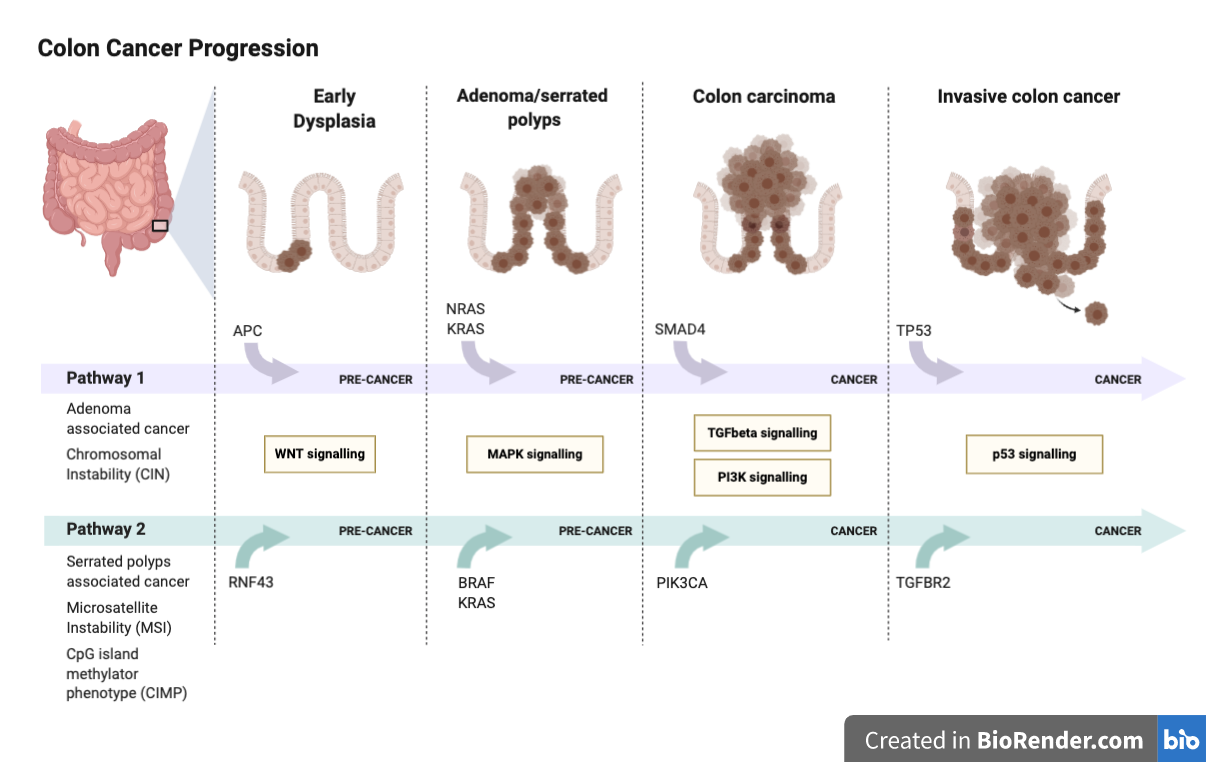
\includegraphics[scale=.35]{figures/colon_cancer_progression.png}
\caption{Colon Cancer Progression}
\label{colon_cancer_progression}
\end{figure}

\subsection{Colorectal Cancer Emergence and Evolution}
According to the adenoma-carcinoma sequence model, the majority of all colorectal adenocarcinomas arise from previously formed adenomas, benign neoplasms of the intestinal epithelium \cite{Cho1992}. Thus, today, one of the most effective medical interventions to reduce death from colorectal cancer is the preventative removal of visible adenomas during lower endoscopy, such as colonoscopy \cite{Nishihara2013Long-TermEndoscopy}.\par

On a molecular level, colorectal adenocarcinoma can be organized into tumors arising through (I) a chromosomal instability or (II) a DNA-mismatch repair deficiency associated route \cite{Markowitz2009} (Figure \ref{colon_cancer_progression}). These two forms of tumor development have been associated with characteristic clinical, pathological and molecular findings. For example, tumors of the DNA-mismatch repair phenotype are more frequently located in the right colon, have a higher proportion of microsatellite instability, frequent BRAF mutations and a higher immune-cell infiltration \cite{Markowitz2009}. In contrast, tumors of the common chromosomal instability (CIN) phenotype are mostly microsatellite stable and have frequent APC and KRAS mutations. \par 

The cascade of genetic events leading to the more frequent chromosomal instability associated form of colorectal cancer cause hyperactivation of a range of signaling pathways. Briefly, this cascade, known as the Vogelstein sequence \cite{Cho1992}, starts with the loss of the tumor suppressor APC in the intestinal epithelium. Loss of APC, which leads to adenoma formation, is followed by the activation of KRAS, PIK3CA, loss of SMAD4 and TP53. Other forms of the disease, especially microsatellite-instable forms of colorectal cancer also harbor mutations of APC but show strong prevalence of BRAF mutations instead of KRAS mutations \cite{Guinney2015TheCancer.}. \par 

Prior studies trying to further define colorectal cancer beyond these two developmental routes have proposed a set of different molecular subtypes \cite{Menter}. In an attempt to unify these models, four consensus molecular subtypes (CMS) have been proposed \cite{Guinney2015TheCancer.}. Briefly, these subtypes organize colorectal cancer into classes defined by (I) a high fraction of microsatellite instable tumors, (II) APC mutations, (III) KRAS mutations and (IV) stromal infiltration, respectively. However, recent evidence has questioned the interpretability of these subtypes in multiple ways. First, the existence of non-malignant cells within the analyzed samples does not allow a direct interpretation of cancer-exclusive molecular processes which might govern treatment response and prognosis \cite{Dunne}. Second, the sampled intra-tumor region and its cellular composition influence the subtype classification result \cite{Dunne2016ChallengingCancer.}. Third, validating studies of the consensus molecular subtype have shown that a large fraction of cancer samples can not be confidently assigned to a single subtype and, more importantly, that subtypes, instead of being well separated, are rather on a high-dimensional continuum. This continuum can be defined by (I) markers of inflammation and T-cell activity and (II) markers of CDK-regulated DNA replication, leading to four quadrants in a continuous space \cite{Ma}. For example, microsatellite instable tumors, which are most frequently found in the first CMS subgroup, were associated with a strong T-cell activity signature and a low CDK-regulated DNA replication signature. Along these lines, immune-cell infiltration has been established as an independent prognostic factor of overall survival and recurrence risk of colorectal cancer and is exploited in immunotherapy, which is especially active in MSI-high tumors \cite{galon, pages}. In contrast, CDK-dependent signaling has recently been recognized as a potential driver of immune-escape in multiple solid cancers \cite{Chaikovsky1}. \par 

In summary, the molecular landscape of colorectal cancer is organized by two distinct forms of tumor development, chromosomal instability and microsatellite instability, that are linked to characteristic genetic changes resulting in a continuum of gene expression states which present themselves with varying degrees of cell proliferation and inflammation. \par

\subsection{Signaling Pathways controlling Colorectal Cancer}
\subsubsection{Wnt signaling in colorectal cancer}
The role of Wnt signaling during colorectal cancer development is well established \cite{Polakis2007}. While activating mutations of \textbeta-catenin do exist, loss of APC is the most frequent driver of Wnt signaling in colorectal cancer and can be found in about 80\% of colorectal cancer patients \cite{Fearon1989}. In line with its role as a tumor suppressor, truncating of APC using the CRISPR/Cas9 technology, leads to colorectal cancer development, which can be modeled ex vivo in human intestinal organoids \cite{Matano2015, Drost2015SequentialCells}. Furthermore, by using a mouse model allowing the reversible knockdown of Apc via shRNA, it was demonstrated that adenomas could regress to normal tissue once APC function is restored, underlining the importance of continuous Wnt signaling for tumor maintenance \cite{Dow2015}. \par
Although loss of APC in general is a driving event of colorectal cancer development and persistence, not every mutation of the APC gene leads to a similar phenotype. Studies of human colorectal cancer samples and tumors from mouse models revealed that different mutations of APC result in distinct levels of canonical Wnt pathway activity and, in addition, are associated with characteristic tumor locations within the large intestine \cite{Christie2013, Buchert2010}. \par

Besides APC, mutations in R-spondin and RNF43, regulators of Wnt receptor abundance at the cell surface level, 
were implicated as drivers of Wnt-dependent tumor growth. Deleterious RNF43 mutations have been described in ~20\% of colorectal cancer cases and are mutually exclusive to APC mutations. Also, amplified R-spondin3 fusion proteins have been described in 10\% of CRC cases. While APC and \textbeta-catenin are generally considered independent of Wnt ligand availability, RNF43 mutant cancers are strongly dependent on Wnt secretion, rendering them highly susceptible to Wnt secretion targeted therapy.

\subsubsection{ERK MAPK Signaling in Colorectal cancer}


In colorectal cancer, the ERK MAPK signaling cascade and its members Ras/Raf/MEK and ERK are key regulators of cell proliferation in malignant cells. The Ras kinase members are mutated in about 36\% of colorectal cancers \cite{Oncol2005}. According to the Vogelstein model of colorectal cancer initiation \cite{Fearon1989}, activating mutations of KRAS takes place early during cancer development, more specifically, after loss of APC.
Next to KRAS, BRAF mutations can also be found in around 10\% of colorectal cancers \cite{Oncol2005}. Of note, mutations of KRAS and BRAF occur mostly in a mutually exclusive pattern with BRAF mutations being enriched in Microsatellite instable colorectal cancers \cite{Oncol2005, Sahin2013}. 

\subsubsection{IGF and mTOR Signaling in Colorectal Cancer}

\subsubsection{TGF beta Signaling in Colorectal cancer}

\subsubsection{TP53 Signaling in Colorectal cancer}

\subsection{Colorectal Cancer Organoid models}

\section{Colorectal Cancer Therapy}
The treatment of colorectal adenocarcinoma depends on disease stage. While surgical removal of the tumor is at the center of the treatment strategy, neoadjuvant and adjuvant chemotherapy are part of the recommended therapy from UICC stage 2 and 4 on, respectively. Today, for metastatic colorectal cancer the first line treatment includes combination chemotherapy (FOLFOX or FOLFIRI) paired with Cetuximab (anti-EGFR) for KRAS wildtype disease, combination chemotherapy with Bevacizumab (anti-VEGFR) for KRAS mutant disease or triple chemotherapy (FOLFOXIRI) in combination with Bevacizumab for BRAF mutant disease \cite{Cutsem}. Following lines of therapy include different combinations of the aforementioned agents with the exception of Regorafenib and Triflouridin/Tipiracil as preferred third line agents for non-KRAS wildtype disease \cite{Cutsem}. Consequentially, the only genetic tests currently recommended during therapy are the determination of KRAS and BRAF status \cite{Cutsem}. Other genetic tests or targeted inhibitors have so far not found their way into clinical practice.\par

Both the important role of adenocarcinoma development and the limitations of personalized therapy in advanced stages of the disease motivated the research presented in this dissertation.

\section{Cancer Drug Discovery}
\subsection{Rational and Functional Drug Discovery}
\subsection{Image-based Profiling}
A challenge for organoid research is the need for information-rich drug-testing methods. In the past, automated microscopy of 2D-cells has been used to measure the biological activity of compounds (Breinig et al. 2015). Prompted by this, we build a platform for high-throughput drug activity profiling in organoids. The platform uses confocal microscopy to collect fluorescent images of treated organoids in 3D. We devel- oped SCOPE, a software package, to process these images and measure organoid phenotypes. We used this platform to test compounds on both patient derived organoids and genetically engineered organoid models.

\section{Aims of Thesis}
\subsection{Image-based profiling of colon organoid models}
\subsection{patient derived organoids identifies compound-induced phenotypes}
\subsection{Multi-omics profiling of intestinal organoids identifies an epistatic relationship of Apc loss and Kras activation during colorectal cancer development}
\end{flushleft}

% First, we isolated and characterized patient derived colorectal cancer organoids. Next, we performed high- throughput drug profiling of these organoids. Here, we observed a variety of recurring treatment-induced phenotypes. These were linked to specific cellular processes. Of note, the treatment response of organoids in-vitro matched the response of donating patients.

% Second, we isolated colon organoids from healthy mouse tissue. By using gene-editing, we generated models of colon adenoma - a precursor lesion of colorectal cancer. These models carried different combinations of mutations in the Apc and Kras gene. Both are frequent and co-occurring mutations in colorectal cancer (Schell et al. 2016). To better understand the mechanisms of tumor development, we performed a multi- omics characterization in these adenoma models. Moreover, we profiled genotype specific drug effects. Here we found a reorganization of organoid phenotype after loss of Apc, which masks the effects of an isolated Kras mutation. Loss of Apc leads to genotype specific drug-induced phenotypes and vulnerabilities. Oncogenic Kras buffers a subset of these vulnerabilities, offering a new perspective on the relationship of Apc and Kras during tumor development.
\begin{savequote}[75mm]
Details matter, it’s worth waiting to get it right.
\qauthor{Steve Jobs}
\end{savequote}

% pending plagiarism check
\begin{flushleft}
\chapter{Materials and Methods}

\section{Patients}
All patients were identified at the University Hospital Mannheim, Mannheim, Germany. We included untreated patients with a new diagnosis of colon or rectal cancer in this study and obtained biopsies from their primary tumors and adjacent normal tissue via forceps based endoscopy. Exclusion criteria were active HIV, HBV or HCV infections. Biopsies were transported in phosphate buffered saline (PBS) on ice for subsequent organoid extraction. Clinical data, tumor characteristics and molecular tumor data were pseudonymized. The study was approved by the Medical Ethics Committee II of the Medical Faculty Mannheim, Heidelberg University (Reference no. 2014-633N-MA and 2016-607N-MA). All patients gave written informed consent before tumor biopsy was performed. In this study, we extracted PDOs from 25 patients with colorectal cancer, 10 of them female, 15 male, with a mean age of 66 years (median 65). 16 patients had a rectum carcinoma, 9 a colon carcinoma.

\section{Organoid Culture}

\subsection{Patient Derived Organoid Culture}
Patient derived organiod (PDO) cultures were extracted from biopsies as reported by Sato et al. \cite{Sato2011-lh} with slight modifications. Tissue fragments were washed in DPBS (Life technologies) and digested with Liberase TH (Roche) before embedding into BME R1 (Trevigen). The medium, termed ENA, contained Advanced DMEM/F12 (Life technologies) medium with 1\% v/v penicillin/streptomycin (Life Technologies), Glutamax and HEPES (basal medium) supplemented with 100 ng/ml Noggin (Peprotech), B27 (Life technologies), 1,25 mM n-Acetyl Cysteine (Sigma), 10 mM Nicotinamide (Sigma), 50 ng/ml human EGF (Peprotech), 10 nM Gastrin (Peprotech), 500 nM A83-01 (Biocat), 10 nM Prostaglandin E2 (Santa Cruz Biotechnology), 10 μM Y-27632 (Selleck chemicals) and 100 mg/ml Primocin (Invivogen). After isolation, cells were kept in 2 conditions including medium as described (ENA), or supplemented with additional 3 uM SB202190 (Biomol) (ENAS) as described by Fujii et al. \cite{Fujii2016ATumorigenesi  }. 
The tumor niche was determined after 14 days and organoids were subsequently cultured in the condition with best visible growth. 
Organoids were passaged every 7 days and medium was changed every 2-3 days.

\subsection{Mouse Organoid Culture}
A heterozygous LSL-Kras G12D (B6.129S4-Krastm4Tyj/J) female mouse was crossed with a homozygous Rosa26-CreERT2 (B6.129-Gt(ROSA)26Sortm1(cre/ERT2)Tyj/J) male to generate offspring with a Tamoxifen activatable KRAS G12D allele. A single healthy LSL-Kras G12D CreERT2 mouse (male, 8 weeks) was sacrificed for organoid generation. 

Mouse colon organoids were isolated based on work by Sato et al \cite{Sato2009-jw}. After cervical dislocation of the sacrificed mouse the colon was prepared and excised between caecum and rectum. The tissue was stored on ice in cooled DPBS (Life technologies), cut open lengthwise and washed three times with DPBS. After thorough washing, colon fragments were cut into 2mm pieces and incubated in a 5mM EDTA/DPBS (Sigma) solution for 60 minutes on a rocking table. Digested fragments were allowed to settle and resuspended in DMEM/F12 (Life technologies) by repeated up- and down-pipetting with a serological pipette. The resulting crypt suspension was filtered with a 70ul filter (Falcon), crypts were counted and centrifuged at 150g, 10min, 4C. The resulting pellet was resuspended in 10mg/ml Matrigel (Corning) and plated on prewarmed 6-well suspension plates (Greiner). After 30-60 minutes of solidification, droplets were overlaid with complete organoid growth medium and incubated at 37C, 5\% CO2 in atmospheric air.

Complete colon organoid medium, termed WENRAS, contained 30\% advanced DMEM/F12 (Life Technologies) supplemented with 1\% v/v penicillin/streptomycin solution (Life Technologies), 1\% v/v HEPES buffer (Life Technologies) and 1\% v/v Glutamax (Life Technologies), 50\% Wnt3A conditioned medium, and 20\% R-spondin1-FC conditioned medium. 
The medium was further supplemented with recombinant Noggin (100 ng/ml), 1x B27 (1x), n-Acetyl-cysteine (1.25 mM), Nicotinamide (10 mM), EGF (50 ng/ml), 500 nM A83-01 (Tocris), SB202190 (3 μM), Y-27632 (10 µM) and Primocin (100 µg/ml). All small molecule inhibitors were dissolved in DMSO. 

After isolation, colon organoids were cultured in solidified BME R1 (10mg/ml) droplets and overlaid with genotype and experiment dependent growth medium. The medium was exchanged every 48-72 h. 
APC mutant colon organoid lines were cultured without Wnt and R-spondin conditioned medium, which was replaced by basal medium instead.
Organoids were passaged weekly by digestion with TrypLE (Gibco) and resuspension in BME R1 (10mg/ml). 
Organoids were regularly tested for Mycoplasma contaminations.  

\subsection{Genetic editing of organoids}
An sgRNA targeting the murine ortholog of the APC mutation cluster region (MCR) was designed using E-CRISP(Heigwer et al., 2014). The Apc targeting sgRNA was cloned into the one-vector plasmid pSpCas9(BB)-2A-Puro (PX459) V2.0 according to Ran et al. \cite{Ran2013}. Briefly, the vector was digested with Bbs1-HF (Thermo) and the phosphorylated and annealed oligonucleotide sgApc1 (sgAPC1 F and -R) was ligated using T4-Ligase (Thermo). The construct was transformed into chemically competent bacterial cells (Stellar, Clontech) and plated on Carbenicillin agar. Individual colonies were isolated and sequencing of plasmid DNA from cultured colonies confirmed successful molecular cloning.   
Extracted organoids (termed “wildtype”, “WT”) were cultured for multiple passages before transfection of the plasmid with Lipofectamine 2000 (Thermo). Here, grown organoids were digested with TrypLE (Gibco) and treated with Lipofectamine and plasmid DNA according to the manufacturer’s protocol. Transfected organoids were seeded in BME R1 (10mg/ml) and Wnt3A/R-Spondin1-Fc withdrawal was started 7 days after transfection. Surviving organoids were cultured continuously without Wnt3A and R-Spondin1-Fc conditioned medium (termed “A”).
To activate oncogenic Kras, Wildtype and APC mutant organoid lines were treated for 7 days with 0.5uM 4-Hydroxytamoxifen (Sigma) without EGF in the medium. 4-Hydroxytamoxifen was dissolved in Ethanol. After treatment, organoids were cultured with EGF containing media thereafter (termed “K” or “AK”, respectively).

\section{Biochemical assays}

%% stopped citing

\subsection{Amplicon Sequencing of Patient derived organoids}
DNA was isolated from 19 organoid cultures with the DNA blood and tissue kit (Qiagen). Sequencing libraries were prepared with a custom panel (Tru-Seq custom library kit, Illumina) according to the manufacturers protocol and sequenced on a MiSeq (Illumina). Targeted regions included the most commonly mutated hot spots in colorectal cancer in 46 genes captured with 157 amplicons of approximately 250bp length. A list of targeted hot- spots that were sequenced can be found in supplementary table S5. After mapping of the reads to GRC38 reference genome using Burrows-Wheeler Aligner (BWA), data were analyzed using the Genome Analysis Toolkit (GATK) (McKenna et al., 2010; Van der Auwera et al., 2013). Base recalibration was performed and variants were called using MuTect2 pipeline. Variants with a variant frequency below 10\%, with less than 10 reads, or with a high strand bias (FS<60) were filtered out. Variants were annotated with Ensemble variant effect predictor (McLaren et al., 2016) and manually checked and curated using integrative genomics viewer, if necessary \cite{Thorvaldsdottir}. Only non-synonymous variants present in COSMIC (Forbes et al., 2015) were considered true somatic cancer mutations.
Also, all variants annotated “benign” according to PolyPhen database and “tolerated” in SIFT database were excluded, as well as variants with a high frequency in the general population as determined by a GnomAD (Lek et al., 2016) frequency of >0.001.

\subsection{Amplicon Sequencing of Mouse Organoids}
Amplicon sequencing was performed to validate the genetic perturbation of Apc. DNA from Apc targeted and untargeted organoid lines was prepared using the DNA Blood and Tissue Kit (Qiagen), according to the manufacturer’s tissue protocol including an RNAse digestion. The targeted region was PCR amplified using primers F1 to R2, and sequencing libraries were prepared according to the manufacturer’s protocol. Libraries were sequenced on a MySeq (Illumina) using 100bp single end reads. 

\subsection{Genomic PCR of KRAS G12D allele}
To confirm activation of oncogenic Kras in 4-Hydroxytamoxifen treated lines, genomic DNA was isolated from all 4 organoid lines as described above. Presence or absence of the Lox-STOP-Lox cassette was evaluated by PCR according to the Kras G12D conditional PCR protocol by Tyler Jacks’ group(Jackson et al., 2001). Briefly, primers #2 and #3 were used for genotyping on genomic DNA using the Q5 PCR protocol (NEB).

\subsection{Western Blot}
Organoids were cultured in Matrigel (Corning). Organoids were collected, and cells were isolated using Matrisperse (Corning) for 40 minutes on a rocking table. Isolated organoids were lysed in RIPA buffer (Sigma) with Protease inhibitor (Sigma) and Phosphatase inhibitor 3 (Sigma). Protein concentration was measured using the Pierce BCA kit (Thermo) according to the manufacturers protocol and samples were loaded onto NuPage gels (Thermo). Western Blotting was performed with following antibodies: anti-p(hospho)-Erk (1:2000), anti-Erk (1:1000), anti-SREBP1 (1:1000), anti-SCAP (1:5000) and anti-beta-actin-HRP (1:150,000).

\subsection{Organoid Growth Patterns}
Organoids were passaged and seeded in 4 different growth media with medium changes every 48h. Images were taken 120h after seeding.  

\subsection{RT-qPCR}
Organoids were passaged and seeded in 4 different growth media with medium changes every 48h. After 120h, organoid RNA was isolated using the RNAEasy Kit (Qiagen) with beta-Mercaptoethanol (Invitrogen) and a DNAse digestion step. cDNA was synthesized using Oligo-dT primers (Thermo), RiboLock Ribonuclease inhibitor (Thermo) and Revert Aid H Minus reverse transcriptase (Thermo). RT-qPCR was performed using the ROCHE UPL kit (Roche), Sdha and Hprt expression levels were used as controls and averaged. Relative transcript abundance was measured using the ddCT method. RT-qPCR primers targeting Axin2, Ccnd, as well as the mouse reference genes Sdha and Hprt were used. 

\subsection{Mass Spectrometry}
Organoids were cultured according to the screening protocol (above). Organoids were isolated with Matrisperse (Corning) as described above. Isolated organoids were lysed in Ammonium Bicarbonate lysis buffer (50mM, pH 8.2) with 2.5\% w/v SDC and 25U/ml Benzonase. 
Samples were applied to 1D-SDS-PAGE and fractionated. Gel pieces were extracted, cysteins residues reduced by DTT and carbamidomethylated using iodoacetamide. The samples were digested with Trypsin overnight.
Resulting peptides were loaded on a cartridge trap column, packed with Acclaim PepMap300 C18, 5µm, 300Å wide pore (Thermo) and segregated in a 60 min gradient from 3\% to 40\% ACN on a nanoEase MZ Peptide analytical column (300Å, 1.7 µm, 75 µm x 200 mm, Waters). Eluted peptides were analyzed by an online coupled Q-Exactive-HF-X mass spectrometer.

\subsection{Expression Profiling}
Organoid RNA was isolated from 19 PDO lines with the RNeasy mini kit after snap freezing organoids on dry ice. Samples were hybridized on Affymetrix U133 plus 2.0 arrays. Raw microarray data were normalized using the robust multi-array average (RMA) method (Irizarry et al., 2003) followed by quantile normalization as implemented in the ‘affy’ (Gautier et al., 2004) R/Bioconductor (Huber et al., 2015) package. In order to exclude the presence of batch effects in the data, principal component analysis and hierarchical clustering were applied. Consensus molecular subtypes were determined as described previously (Guinney et al., 2015) using the single sample CMS classification algorithm with default parameters as implemented in the R package ‘CMSclassifier’. In all cases, differential gene expression analyses were performed using a moderated t-test as implemented in the R/Bioconductor package ‘limma’ (Ritchie et al., 2015). Gene set enrichment analyses were performed using ConsensusPathDB (Kamburov et al., 2013) for discrete gene sets or GSEA as implemented in the ‘fgsea’ (Sergushichev, 2016; Subramanian et al., 2005) R/Bioconductor package for ranked gene lists.

Mouse organoids were cultured according to a standardized screening protocol. Briefly, organoid models were seeded and cultured for 72h in WENRAS+Y and additional 96h in ENR-Y. Samples were harvested after 7 days and RNA was isolated using the RNAEasy Kit (Qiagen) as described above. Transcript expression levels were measured using MoGene-2\_0-st chips (Affymetrix).    

\section{Organoid profiling}

\subsection{Cell Seeding during Compound testing}
PDO drug profiling followed a standardized protocol with comprehensive documentation of all procedures. Organoids were collected and digested in TrypLE Express (Life technologies). Fragments were collected in basal medium with 300 U/ml DNAse and strained through a 40μm filter to achieve a homogeneous cell suspension with single cells and small clusters of cells, but without large organoid fragments. 384 well μclear assay plates (Greiner) were coated with 10μL BME V2 (Trevigen) at a concentration of 6.3 mg/ml in basal medium, centrifuged and incubated for >20 min at 300G and 37° C to allow solidification of the gel. PDO cell
clusters together with culture medium (ENA) and 0,8 mg/ml BME V2 were added in a volume of 50μl per well using a Multidrop dispenser (Thermo Fisher Scientific). Plates were sealed with a plate-loc (Agilent) and centrifuged for additional 20 min allowing cells to settle on the pre-dispensed gel. Cell number was normalized before seeding by measuring ATP levels in a 1:2 dilution series of digested organoids with CellTiter-Glo (Promega). The number of cells matching 10,000 photons was seeded in each well. After seeding of organoid fragments, plates were incubated for three days at 37°C to allow organoid formation before addition of compounds. Two biological replicates of each PDO line from different passages were profiled at different time points.

Mouse organoid screening was performed as described above with slight modifications. Clotting of organoid fragments was avoided by adding 10 U/ml of bovine DNAse1 to the medium during filtration. The cell viability of digested fragment suspensions was estimated using Cell-Titer-Glo (Promega). 40ul of cell suspension was mixed with 40ul of undiluted reagent and measured after 30 minutes on a Mithras plate reader (Berthold). Cell fragments with a viability corresponding to 5000 photons were seeded per well on pre-coated 384 well plates using a Multidrop peristaltic pump robot (Thermo). After 72 hours of organoid expansion in WENRAS+Y, the medium was changed to ENR-Y and compound libraries were added using a BiomekFX (Beckmann). Screening plates were further incubated for 96h before a cell permeability dye Image-IT DeadGreen was added for 4 hours and cells were fixed in a 3\% PFA buffer supplemented with 1\% BSA. After fixation, plates were stored for up to 4 days or directly stained with DAPI (Sigma) and Phalloidin-TRITC. Processed plates were imaged using an Incell6000 automated line-scanning confocal fluorescence microscope.

\subsection{Compound Libraries}
Two compound libraries were used for screening: A library containing 63 clinically relevant drugs (clinical cancer library) and a large library of 464 compounds targeting kinases and stem cell or developmental pathways associated genes (KiStem library). The clinical cancer library was manually curated by relevance for current (colorectal) cancer therapy, mechanism of action and potential clinical applicability. Compounds of this library are in clinical use or at least in phase I/II clinical trials. Five concentrations per compound were screened (five-fold dilutions). The concentrations were determined by analysis of literature data from previous 3D and 2D drug screens and own experiments. A list of compounds included in this library and maximum concentrations used can be found in S3. The KiStem library includes 464 compounds targeting a diverse set of kinases and stem cell relevant pathways S4. All compounds in this library were used in a concentration of 7.5μM. All compounds were obtained from Selleck chemicals. Compounds of both libraries were arranged in an optimized random layout. We stored compound libraries in DMSO at -80 C.

\subsection{Compound Treatment}
Medium was aspirated from all screening plates and replaced with fresh ENA medium devoid of Y-27632, resulting in 45μl volume per well. Drug libraries were diluted in basal medium and subsequently 5μl of each compound was distributed to screening plates. 
All liquid handling steps were performed using a Biomek FX robotic system (Beckmann Coulter). Plates were sealed and incubated with the compounds for four days. All PDO lines underwent profiling with the clinical cancer library, while the KiStem library was used with 13 PDO lines.

\subsection{Luminescence Viability Read Out}
Plates undergoing viability screening were treated with 30μl CellTiter-Glo reagent after medium aspiration with a Biomek FX. After incubation for 30 minutes, luminescence levels were measured with a Mithras reader (Berthold technologies).

For mouse experiments, before compound addition, organoid viability was measured using Cell-Titer-Glo (Promega) and WENR-Y was added to the remaining plates. Cell viability was measured after compound exposure as described above. The pre-treatment viability of organoids was used to estimate growth-rate controlled dose-response curves according to Clark et al.(Hafner et al., 2016) Measurements of GR metrics for was not robust for slow proliferating WT lines. Therefore, we omitted plotting dose-response curves for WT lines when a GRfit was conducted. Dose response curves of relative viability, including the WT line can be found in the supplementary figures. 

\subsection{Image-based Phenotyping}
Image-IT DeadGreen (Thermo Fisher) was added to the cultures with a Multidrop dispenser (Thermo Fisher) in 100nM final concentration and incubated for four hours. Afterwards, medium was removed and organoid cultures were fixed with 3\% PFA in PBS with 1\% BSA. Fixed plates were stored at 4° C for up to three days before permeabilization and staining. On the day of imaging, organoids were permeabilized with 0.3\% Triton-X-100 and 0.05\% Tween in PBS with 1\% BSA and stained with 0.1μg/ml TRITC-Phalloidin (Sigma) and 2μg/ml DAPI (Sigma). All liquid handling steps were performed with a BiomekFX. Screening plates were imaged with an Incell Analyzer 6000 (GE Healthcare) line-scanning confocal fluorescent microscope. We acquired 4 fields per well with z-stacks of 16 slices at 10x magnification. The z-steps between the 16 slices had a distance of 5μm, the depth of field of each slice was 3.9μm.

\subsection{Immunohistochemistry}
PDOs were fixed for 20 min in 4\% (v/v) Roti Histofix (Carl Roth) followed by embedding into MicroTissues 3D Petri Dish micromolds (Sigma Aldrich) using 2\% (w/v) Agarose LE (Sigma) in PBS supplemented with 0.5 mM DTT. Thereafter, PDOs were subjected to dehydration steps and embedding in paraffin. Formalin-Fixed Agarose/Paraffin-Embedded sections (3- 5μm) were manually cut from blocks with a microtome (Leica RM 2145) and transferred to glass slides (Superfrost, Thermofisher Scientific) before H&E staining using automated staining devices.

\subsection{Proliferation Assay}
Organoids were collected, digested, strained, normalized and seeded as in the drug profiling protocol described above. Medium change was performed on days 2 and 4. Viability of plated organoids was measured 2, 4 and 8 days after seeding using CellTiter-Glo as described above.

\section{Image analysis}

\subsection{Image Processing}
Microscopic image z-stacks were compressed to HDF5 format for archival and underwent maximum contrast projection using the R/Bioconductor package MaxContrastProjection for further processing of the images. Segmentation of the projections based on intensity did not sufficiently identify organoids. Instead, we trained a deep convolutional neural network (DCNN) on the partially correct intensity segmentation, leveraging the robustness of DCNNs with regards to mislabeled training data and eliminating the need for expensive manual annotations. Standard image features, including shape, moment, intensity, and Haralick texture features on multiple scales, were extracted using the R/Bioconductor package EBImage (Pau et al., 2010). Of note, the strong diversity of unperturbed organoid phenotypes between PDO lines did not allow the definition of a core set of individual reproducible descriptive features across all screened organoids. Therefore, no correlation-based filtering of features was done, allowing comparisons between different PDO lines. Out-of-focus objects were programmatically removed from the dataset using a feature based random forest classifier. Two PDO lines (D015T01 and D021T01) had to be excluded from analysis because of too many of out-of-focus elements.

\subsection{Drug-Induced Phenotypes}
A principal component analysis (PCA) was performed on the entire dataset to reduce the dimensionality. 25 principal components were selected, explaining approx. 81\% of the total variance within the dataset. A linear support vector machine (SVM) was trained per line and treatment (and per concentration where applicable) to differentiate treated organoids from negative controls based on the PCA-transformed features (Loo et al., 2007). To allow comparison between various PDO lines and drug perturbations, the distributions of features describing organoids from different batches were adjusted. Drugs were categorized as either active or inactive based on the accuracy of the SVM. The histogram of accuracies made a threshold of 85\% the most intuitive. The direction of the vector perpendicular to the SVM hyperplane was interpreted as the drug-induced effect. Drugs were clustered with regard to the angles of their corresponding effect vectors in PCA-feature space.

\subsection{Live-Dead Classification}
A random forest classifier was trained on the original single organoid features to differentiate living from dead organoids. Organoids treated with DMSO were used as negative (i.e. living) controls while organoids treated with Bortezomib and SN-38 at the two highest concentrations were used as positive (i.e. dead) controls. Visual inspection of the projected images confirmed our choice of positive controls. Binary classification results were averaged within wells to obtain viability scores ranging from 0 to 1, indicating how lethal a treatment was. A separate classifier was trained for each individual line to ensure inter-line independence.

\subsection{Analysis of Luminescence Data and Dose-Response Relationships}
Raw luminescence data of each plate were first normalized using the Loess-fit method
(Mpindi et al., 2015) in order to correct for edge effects where increased luminescence intensity was observed along the edges of each plate. Subsequently, each plate was normalized by division with the median luminescence intensity of the DMSO controls. Drug response Hill curves (DRC) were fitted and area under the curve values were calculated for each DRC using the ‘PharmacoGx’ (Smirnov et al., 2016) R/Bioconductor package.

\end{flushleft}
\begin{savequote}[75mm]
Often when works at a hard question, nothing good is accomplished at the first attack. Then one takes a rest, long or short, and sits down anew to the work. During the first half-hour, as before, nothing is found, and then all of a sudden the decisive idea presents itself to the mind.
\qauthor{Henri Poincare}
\end{savequote}

% pending plagiarism check
\begin{flushleft}
\chapter{Profiling of organoids identifies molecular determinants of cancer organoid architecture and plasticity}

\newpage


\section{Disclosure}
Significant parts of this chapter have been adapted from own manuscripts, including \textit{The drug-induced phenotypic landscape of colorectal cancer organoids} \cite{Betge2022-kr}. The maximum contrast projection method, organoid segmentation method, feature extraction procedure and organoid viability classification (LDC) were previously developed by Jan Sauer as part of his dissertation \cite{noauthor_undated-ij}. Image-based profiling experiments were supported by Johannes Betge. 

\section{Image-based profiling captures the morphological diversity of patient-derived cancer organoids}

To better understand the diversity of organoid phenotypes and how morphology links to molecular processes, I performed image-based profiling at single organoid resolution with 11 organoid models using compounds targeting developmental pathways (464 compounds), as well as compounds in clinical use (63 compounds in 5 concentrations) together with Johannes Betge (Figure \ref{fig_137} a and b). The resulting data comprised morphological profiles for each organoid with 528 phenotypic features  that were subsequently reduced into 25 principle components representing 81\% of morphological variance.

\begin{figure}[h]
\centering
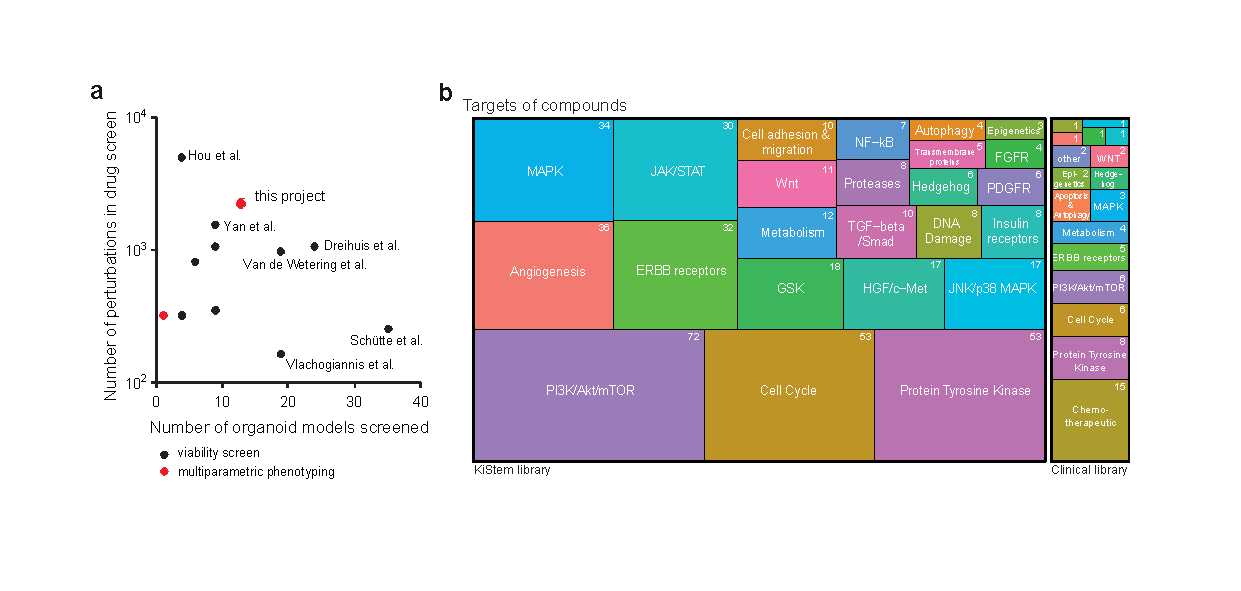
\includegraphics[width=\textwidth,
                height=\textheight,
                keepaspectratio]{figures/promise/pdf/fig_1_3.pdf}
\caption{\textbf{Dataset dimensions and compound library overview a} Number of organoid models and number of perturbations in previous publications reporting high-throughput drug screenings with patient derived cancer organoids, \textbf{b} Graphical representation of the compound libraries used for drug screening in this project: A library targeting kinases and stem cell pathways (KiStem library, 464 compounds) and a clinical library with 63 drugs in 5 concentrations. Figure created with support from Johannes Betge}
\label{fig_137}
\end{figure}

To visualize the heterogeneity of colorectal cancer organoids and drug induced changes across and within cancer organoid lines, the features of ca. 5.5 million profiled organoids were embedded using uniform manifold approximation and projection (UMAP) (Figure \ref{fig_140} a and \ref{fig_145} a-c). Most organoid lines showed characteristic bimodal log-normal distributions of organoid size with one component containing small organoids and another component made up of larger organoids with varying, line specific, average size (Figure \ref{fig_140} b, and \ref{fig_145} d-e). The log-normal-like size distribution likely resulted from intrinsic differences in cellular size and growth rate compounding over time in multicellular organoids. 

\smallbreak
While DNA and Actin staining intensity were positively correlated with organoid size, cell permeability was negatively correlated and enriched in regions with relatively smaller organoids (Figure \ref{fig_145} a-c). Graph-based clustering of this identified 12 regions within the embedding (Figure \ref{fig_140} c). When comparing drug-treated organoids to organoids treated with the negative control (DMSO), no clear separation of these two groups, except an increased presence of drug-treated organoids in region 3,  was seen. This finding suggested that organoid morphology was distributed on a continuum of phenotypes spanning perturbed and unperturbed conditions of the experiment (Figure \ref{fig_145} f). 

\clearpage

\begin{figure}[h]
\centering
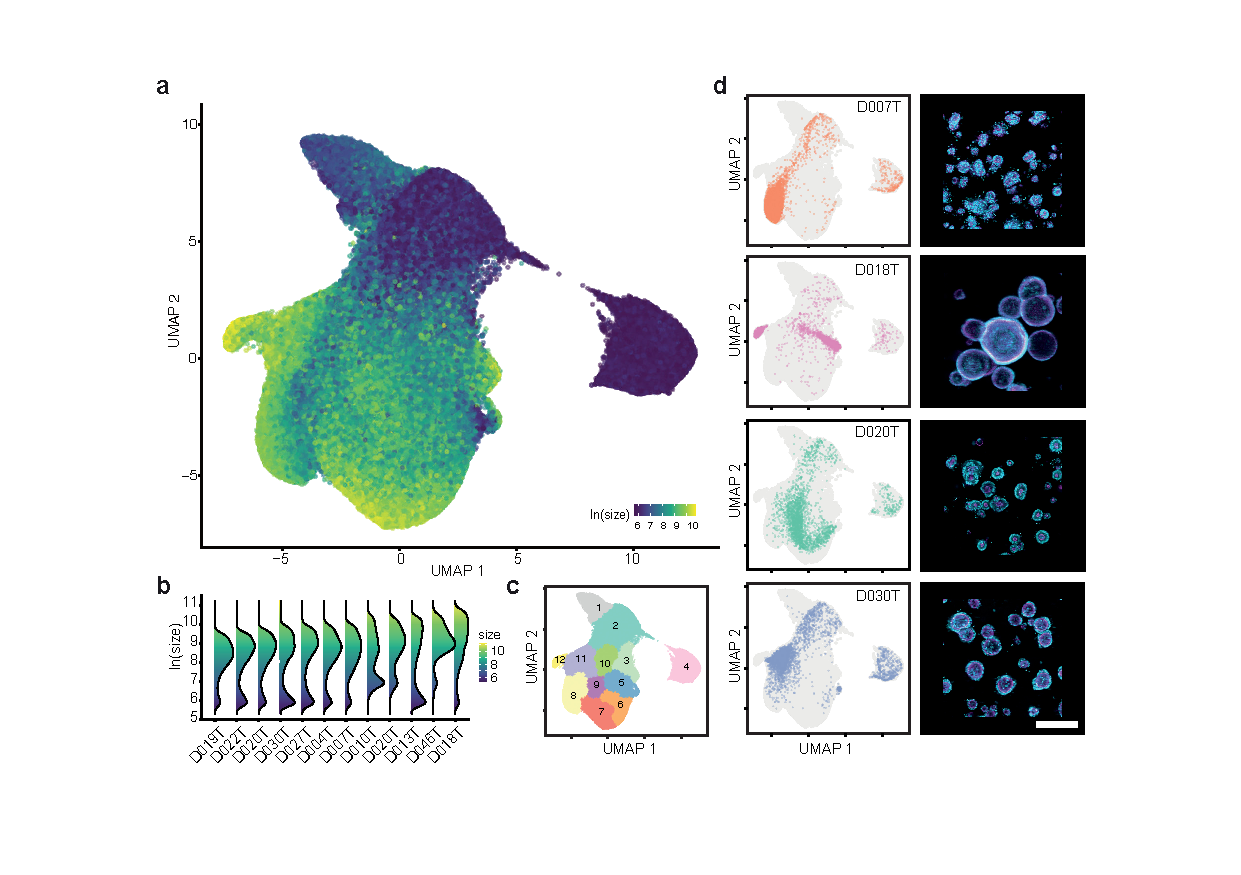
\includegraphics[width=\textwidth,
                height=\textheight,
                keepaspectratio]{figures/promise/pdf/fig_1_4.pdf}
\caption{\textbf{Image-based profiling captures the phenotype diversity of patient derived cancer organoids a} Uniform Manifold Approximation and Projection (UMAP) of organoid-level features for a random 5\% sample out of ca. 5.5 million organoids. The same sample is used for visualizations throughout the figure. Color corresponds to the log-scaled organoid area (dark blue: minimum size, yellow: maximum size). \textbf{b} organoid size distribution across lines. \textbf{c} UMAP representation of DMSO treated and drug treated organoids. Graph-based clustering of organoids by morphology. \textbf{d} UMAP embeddings of selected organoid lines (baseline state / 0.1\% DMSO control-treated organoids) representing different morphological subsets, grey background consists of randomly sampled points. Depicted are representative example images for each line (right, cyan = DNA, magenta = Actin, scale-bar: 200µm).}
\label{fig_140}
\end{figure}
\bigbreak

Different organoid lines within the embedding were located in characteristic regions, with organoid size and organoid architecture as primary organizing factors (Figure \ref{fig_140} b and d). For example, organoid line D018T had the largest median organoid size within the dataset and a cystic organoid architecture, while D020T organoids had a solid architecture and smaller median size. In most cases, organoid lines had two areas of main density, with one of them in regions 2, 3 or 4, reflecting the previously mentioned bimodal size distribution. In summary, image-based profiling of patient derived colorectal cancer organoids showed strong morphological heterogeneity with line dependent differences in size and organoid architecture.

\begin{figure}[h]
\centering
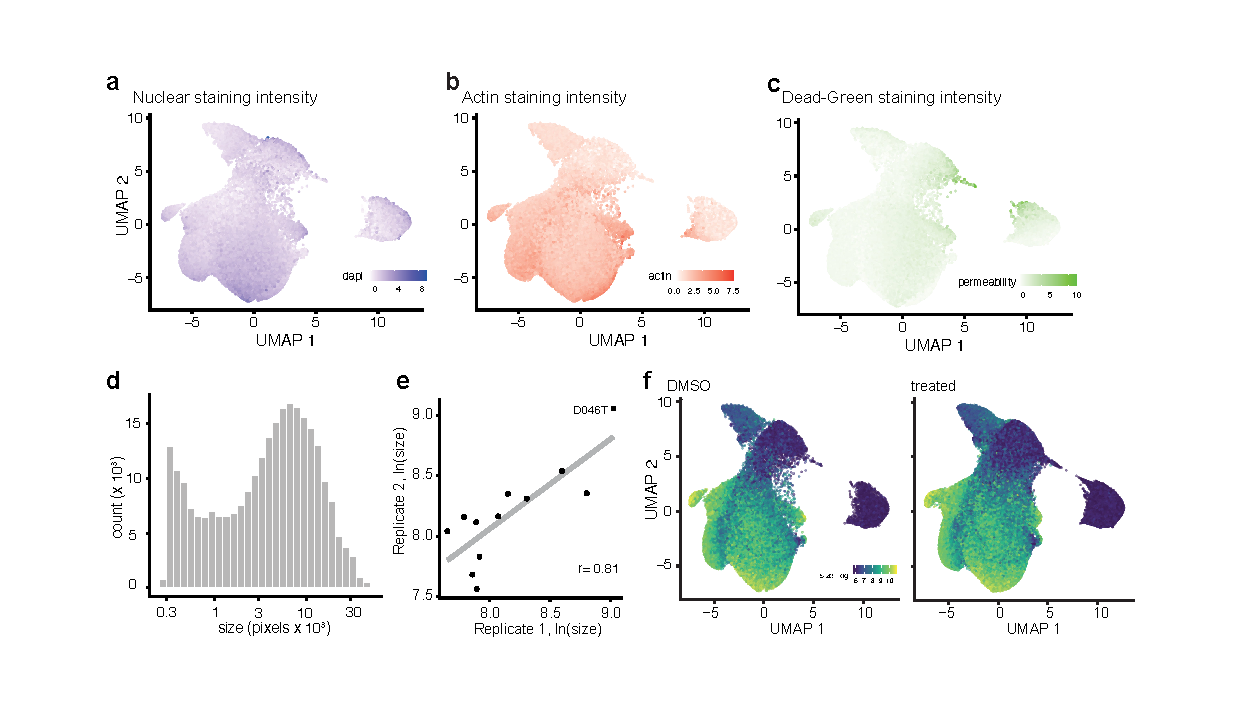
\includegraphics[width=\textwidth,
                height=\textheight,
                keepaspectratio]{figures/promise/pdf/fig_1_5.pdf}
\caption{\textbf{Basic image-based features and their role in organoid phenotype diversity. a-c} Uniform Manifold Approximation and Projection (UMAP) of organoid-level features marked by DNA (DAPI) staining intensity (b), actin (Phalloidi/FITC) staining intensity (c) and permeability (DeadGreen) staining intensity \textbf{d} Distribution of organoid size for all control (DMSO) treated organoids. \textbf{e} Replicate correlation of organoid size for control treated organoids. \textbf{f} UMAP representation of DMSO treated and drug treated organoids}
\label{fig_145}
\end{figure}
\bigbreak

Exploratory data analysis of the relationship between organoid morphology and experimental batch showed overall reproducible measurements of organoid profiles across experiments (Figure \ref{fig_145} e). While objects with a log-area of 8 pixels and larger showed reproducible phenotypes across contexts, smaller objects (mostly dead organoids) showed batch-dependent differences in phenotype.

\smallbreak
For example, region 1 within the UMAP embedding was exclusively occupied by observations from batch HC1092-09 and HC1092-10, while region 4 was relatively underoccupied (Figure \ref{fig_216} a). Given the confounding of line differences by experimental batches (experimental batches and tested organoid lines were not independent) and the stronger prevalence of batch effects for small objects, no procedure to remove these batch-dependent differences in organoid phenotype were performed. 

\bigbreak

\begin{figure}[h]
\centering
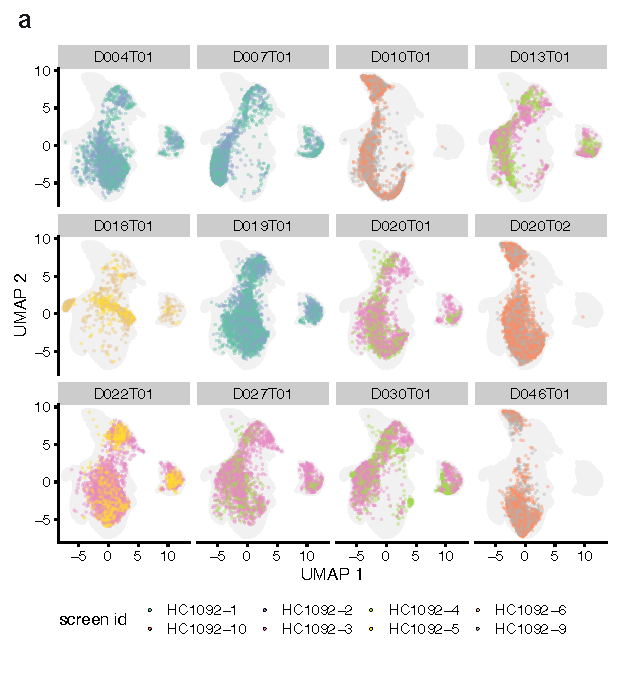
\includegraphics[width=\textwidth,
                height=\textheight,
                keepaspectratio]{figures/promise/pdf/fig_1_6.pdf}
\caption{\textbf{Experimental batches and their impact on organoid phenotype. a} UMAP of organoid level features stratified by organoid line and colored by experimental batch.}
\label{fig_216}
\end{figure}
\clearpage


\section{Organoid phenotype-profiles capture organoid viability}

Drug induced changes in cell viability are a basic readout in oncology drug discovery. Prompted by the observation that organoid size was a major factor determining the structure of the phenotype embedding (UMAP and factor 1 in MOFA analysis, see below), I hypothesized that low organoid size was at least partially the result of cell death within the organoid and, more broadly, that phenotype data could be used to estimate organoid viability. Bortezomib, a small molecule proteasome inhibitor with high in-vitro toxicity led to dose dependent organoid death in all organoid lines, thus representing suitable positive controls (Figure \ref{fig_221} a). Analogous to pseudotime in single-cell  gene expression analysis, dose-dependent trajectories of Bortezomib drug response could be fitted (Figure \ref{fig_221} b) using the non-parametric principle curve method. Starting from diverse baseline morphologies, increasing doses of Bortezomib led to a step-wise convergence on a final death-related phenotype, which corresponded to the areas with enrichment of small objects (regions 2, 3 and 4). 

\begin{figure}[h]
\centering
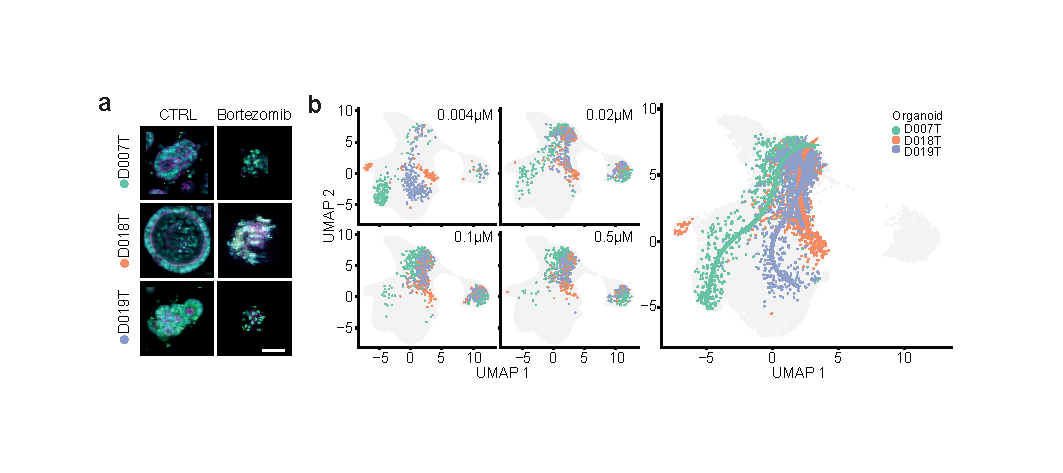
\includegraphics[width=\textwidth,
                height=\textheight,
                keepaspectratio]{figures/promise/pdf/fig_2_1.pdf}
\caption{\textbf{Organoid phenotype-profiles capture organoid viability. a} Representative example images of negative- (0.1\% DMSO) and positive control treated organoids (2.5µM bortezomib, cyan = DNA, magenta = actin, yellow = cell permeability; average images were selected and embedded in black background; scale bar: 50µm). b, Dose-dependent-trajectory of bortezomib drug effect. UMAP of organoid morphology at different bortezomib doses and (right panel) dose-dependent trajectory for three representative organoid lines. For visual purposes, trajectory inference was limited to partition 1, the left-hand set of measurements within the UMAP, representing ca. 95 \% of all imaging data.}
\label{fig_221}
\end{figure}
\bigbreak

Similarly, Paclitaxel, a microtubule disassembly inhibitor, shifted the bimodal size distribution of organoids in a dose-dependent fashion (Figure \ref{fig_222} a), while organoid count remained largely unchanged (Figure \ref{fig_222} b). This effect, however, was organoid line-specific, as median organoid size in Paclitaxel sensitive lines (e.g. D022T) decreased, while the size of other organoids remained unaffected (e.g. D046T, Figure \ref{fig_222} c-f). These observations suggested a link between organoid morphology, especially organoid size, with a loss of cell viability. 

\bigbreak
To further test the link between organoid morphology and cell viability, I performed a luminescence-based, ATP dependent, cell viability assays (CTG) in parallel with imaging as benchmark. A correlation of CTG viability with organoid size (r = 0.64) (Figure \ref{fig_222} a) was visible. 

\begin{figure}[H]
\centering
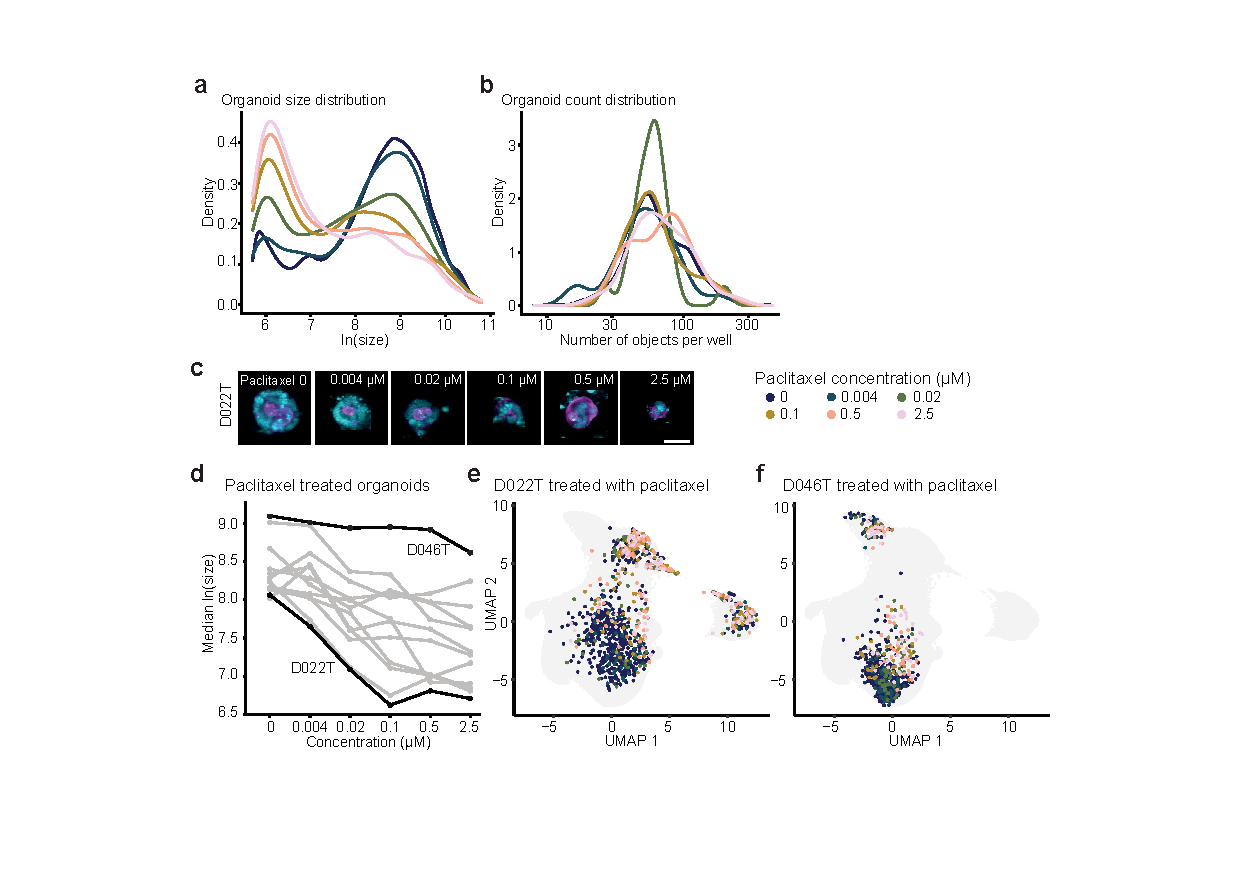
\includegraphics[width=\textwidth,
                height=\textheight,
                keepaspectratio]{figures/promise/pdf/fig_2_2.pdf}
\caption{\textbf{Organoid phenotype-profiles capture treatment specific changes in organoid viability. a} Distribution of organoid size at different concentrations of Paclitaxel. Shown is a random sample of 30\% of all Paclitaxel treated organoids for this and following figures. \textbf{b} Distribution of organoid number per well at different concentrations of Paclitaxel. \textbf{c} Example images of D022T organoids treated with Paclitaxel. \textbf{d} Dose-response relationship of organoid size and paclitaxel dose. D022T and D046T are highlighted. \textbf{e} UMAP of organoid morphology highlighting D022T organoids treated at different concentrations of Paclitaxel. \textbf{f} UMAP of organoid morphology highlighting D046T organoids treated at different concentrations of Paclitaxel.}
\label{fig_222}
\end{figure}
\bigbreak

To test whether a more accurate prediction of organoid viability was achievable by using all available imaging data, I used a previously trained set of random forest classifiers (live/dead classifiers, LDC). These classifiers were trained on individual organoid phenotype profiles to distinguish between negative and positive control treatments (DMSO, Bortezomib and SN-38). 

\bigbreak
When applying the classifier to the whole imaging dataset and visualizing predictions via UMAP, organoids within previously identified small-object regions 2, 3 and 4 had the highest probabilities for death (Figure \ref{fig_222} b). 

\bigbreak
Not only organoid size, but also the viability classified (LDC) correlated with luminescence-based viability (CTG) measurements (Figure \ref{fig_222} b and c). In fact, the trained classified, together with organoid size showed the most robust correlation with luminescence-based viability measurements across all profiled organoid lines (Figure \ref{fig_222} d), while other simple features, such as DAPI, Actin, and permeability (DeadGreen) intensity were less suitable to predict the viability of organoids. 

\bigbreak
In conclusion, organoid size is an informative metric to approximate organoid viability, but is biased by line-specific differences organoid size. Models consuming more comprehensive morphological information can achieve even higher predictive performance of organoid viability. 

\clearpage
\begin{figure}[h]
\centering
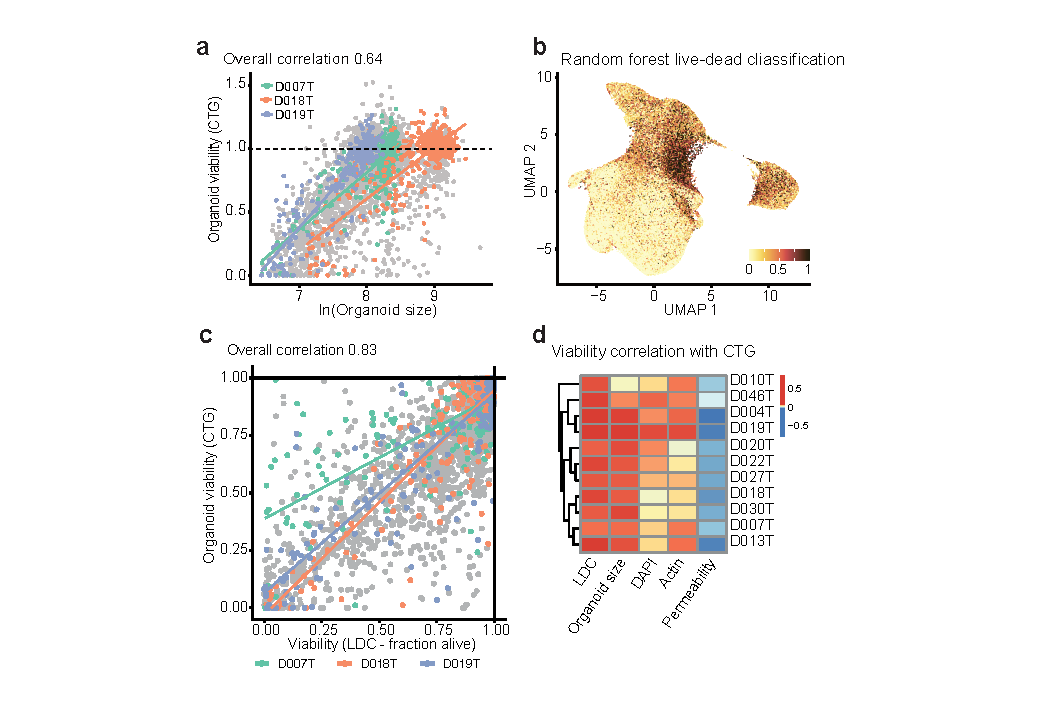
\includegraphics[width=\textwidth,
                height=\textheight,
                keepaspectratio]{figures/promise/pdf/fig_2_3.pdf}
\caption{\textbf{Organoid phenotype-profiles reflect ATP-dependent viability measurements. a} Association of organoid size of selected example lines with organoid viability determined by luminescence-based, ATP-dependent viability profiling with CellTiter-Glo (CTG), which was performed in parallel with imaging on a subset of drug treatments. \textbf{b} UMAP visualization of dead organoids within our dataset, based on supervised machine learning of organoid viability using classifiers trained on positive- (high-dose bortezomib and SN-38) and negative (DMSO) controls (live-dead classifiers, LDC). \textbf{c} Association of organoid size of selected example lines with organoid viability determined by luminescence-based, ATP-dependent viability profiling with CellTiter-Glo (CTG), which was performed in parallel with imaging on a subset of drug treatments for benchmarking. \textbf{d} UMAP visualization of dead organoids within our dataset, based on supervised machine learning of organoid viability using classifiers trained on positive- (high-dose Bortezomib and SN-38) and negative (DMSO) controls (live-dead classifiers, LDC). \textbf{e} Association of LDC and example organoid features (size, DAPI, actin and permeability dye intensities) with benchmark CTG viability read out. Figure created with support from Jan Sauer (LDC classifier training)}
\label{fig_223}
\end{figure}
\bigbreak

\section{Drug induced organoid phenotypes correspond to drug mechanism of action}

An advantage of image-based phenotyping over cell viability measurements in drug discovery is the ability to use the high dimensional drug-induced phenotype-profiles to identify active but not necessarily lethal drugs and estimate their mechanism of action by unsupervised clustering. 

\bigbreak
To test whether this approach could be used in cancer organoids, I used a weakly supervised learning approach to identify drug effect vectors and group them by similarity. With the support of Jan Sauer, logistic regression models to separate individual compound-treated organoids from unperturbed controls were trained. The resulting normal vector between control- and treated organoid profiles was referred to as the drug effect vector. Next I scored every model’s ability to separate treated and untreated organoids (AUROC, ranging from 0.5 to 1) to identify active treatments that induce a robust change in organoid morphology (Figure \ref{fig_230} a, b). Drug activity was necessary but not sufficient for a viability effect (Figure \ref{fig_230} c). A fraction of drugs led to identifiable changes in organoid morphology but were not classified as lethal by our LDC model. 

\begin{figure}[h]
\centering
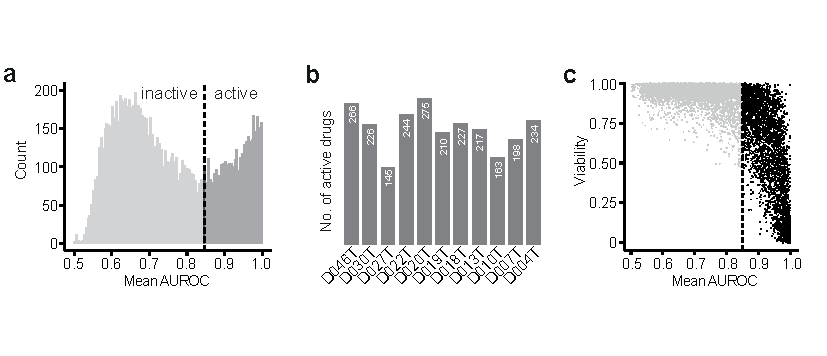
\includegraphics[width=\textwidth,
                height=\textheight,
                keepaspectratio]{figures/promise/pdf/fig_3_0.pdf}
\caption{}
\label{fig_230}
\end{figure}
\bigbreak

To test whether active drugs systematically lead to organoid phenotypes that are informative of mechanism of action, the cosine distance between concatenated drug effect vectors was determined. This approach led to a clustering of specific mode-of-actions, including inhibitors of MEK, Aurora kinase, CDK, mTOR, AKT, EGFR or GSK3 (Figure \ref{fig_231} a). 

\bigbreak
I next validated the previous approach. The AUROC metric which was used to define active treatments, correlated with the eucledian distance of phenotype profiles (Figure \ref{fig_232} a) and showed moderate variation when evaluated for stability using bootstrapping (Figure \ref{fig_232} b). Evaluating an alternative clustering method based on phenotype profile averaging followed by pearson correlation led to similar results to the previous clustering (Figure \ref{fig_232} c). 

\begin{figure}[h!]
\centering
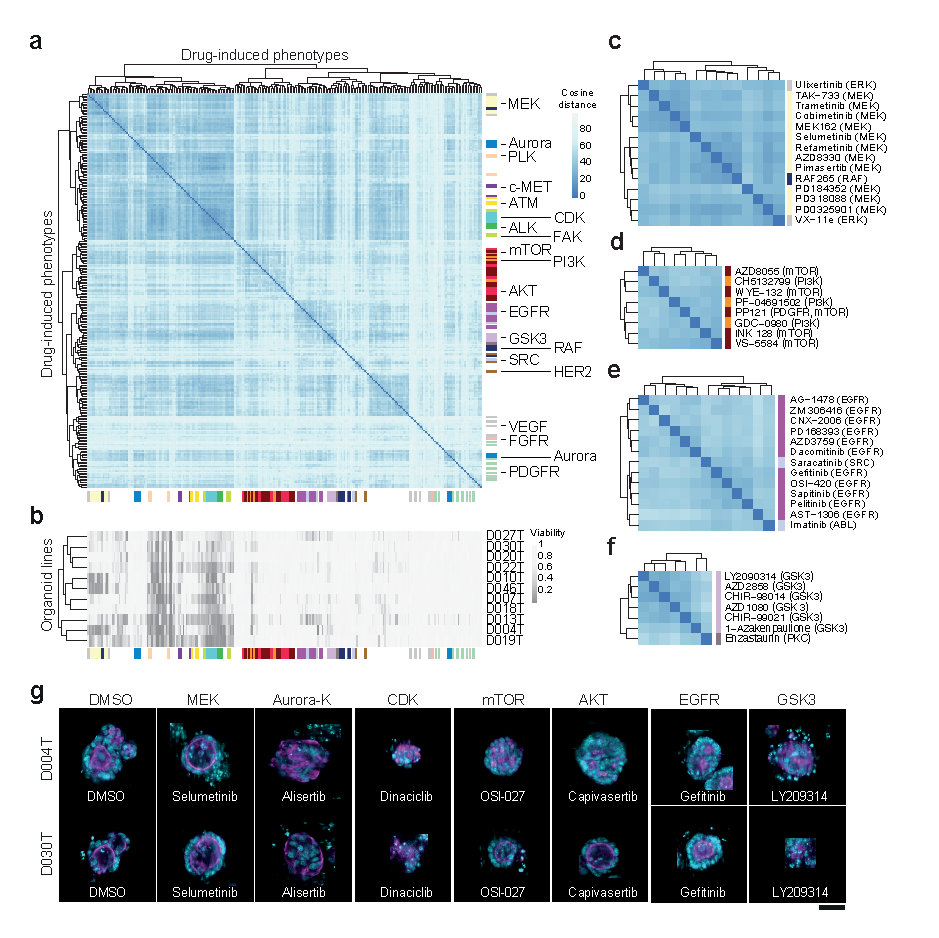
\includegraphics[width=\textwidth,
                height=\textheight,
                keepaspectratio]{figures/promise/pdf/fig_3_1.pdf}
\caption{}
\label{fig_231}
\end{figure}
\bigbreak

Compounds with related, but not identical, targets also induced related phenotypes, for example MEK inhibitors clustered with specific RAF- and ERK inhibitors (Figure \ref{fig_231} c-f) or AKT and PI3K inhibitors were part of a cluster mainly containing mTOR targeting compounds. The clustering also suggested additional mode-of-actions or off-target effects for well-described compounds. For example, the PKC inhibitor enzastaurin was related to GSK3 inhibitors, substantiating a previously described interaction with the alpha and beta subunits of GSK3 28 (Figure \ref{fig_231} f). 

\bigbreak
To assess whether morphological profiles of active drug treatments were primarily driven by differences in organoid viability, we compared viability predictions with the phenotypic clustering (Figure \ref{fig_231} b). While a large cluster of lethal treatments (including molecules targeting ATM, JAK, PLK, CDK) existed, the majority of clusters were caused by non-lethal phenotypes - including those induced by inhibitors of AKT, mTOR, EGFR or GSK3.

\bigbreak
Visual inspection of several phenotypes (Figure \ref{fig_231} g) revealed recurring drug target dependent phenotypes. Most notably, MEK inhibitors led to reorganization towards more cystic organoid architecture. These drug target dependent phenotypes were observable across organoid lines and drugs.

\begin{figure}[h!]
\centering
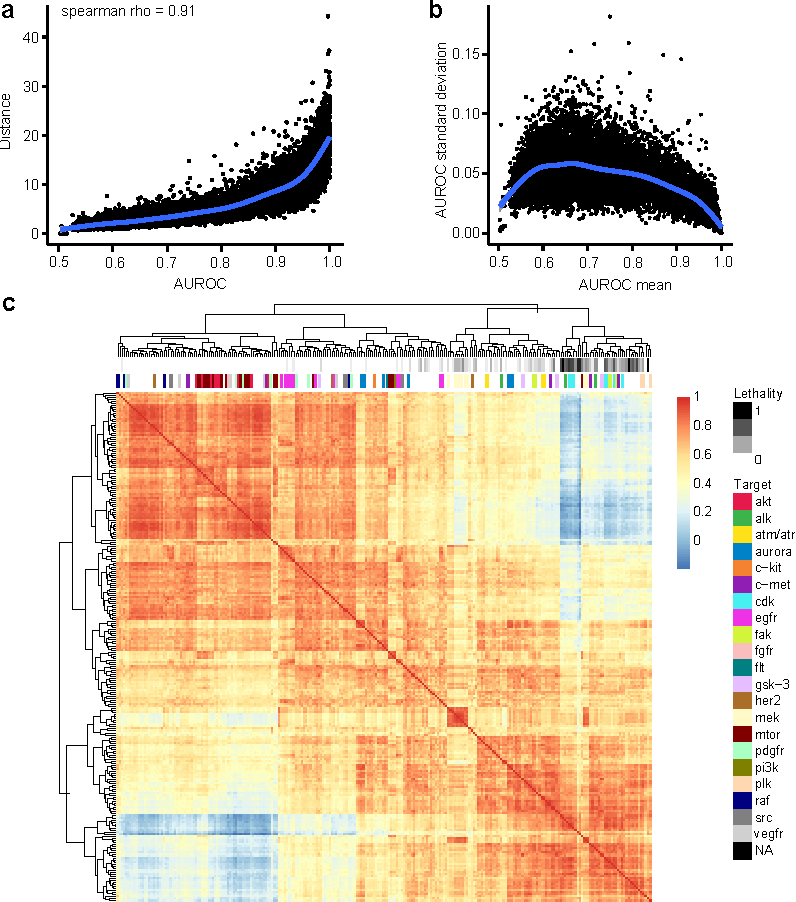
\includegraphics[width=\textwidth,
                height=\textheight,
                keepaspectratio]{figures/promise/pdf/fig_3_2.pdf}
\caption{}
\label{fig_232}
\end{figure}
\bigbreak

% \begin{figure}[h!]
% \centering
% 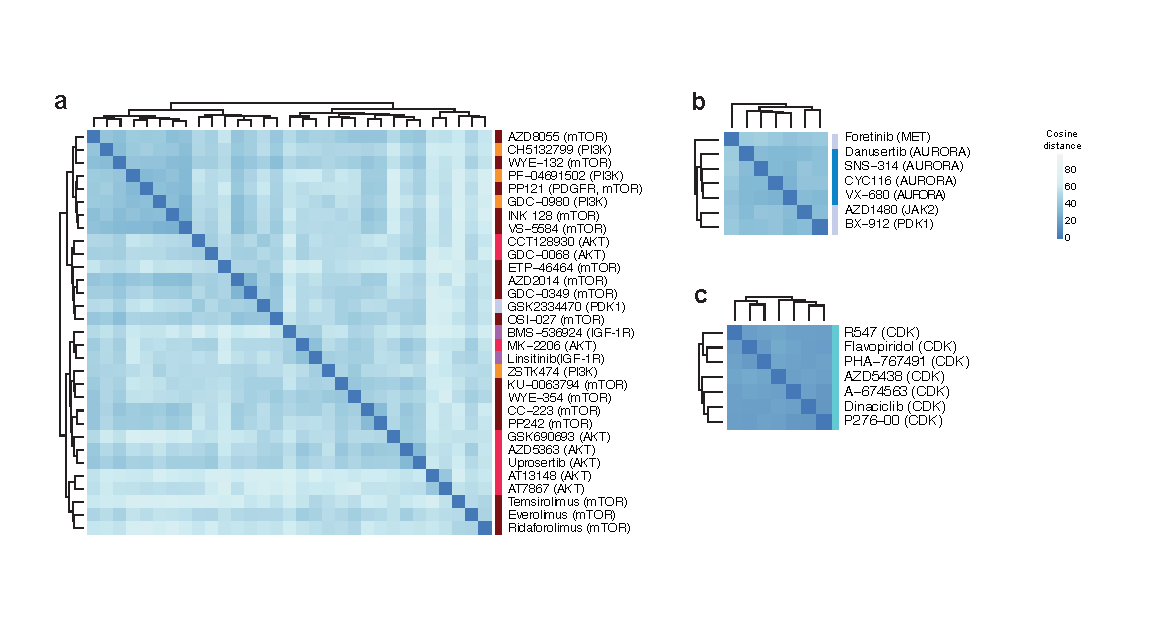
\includegraphics[width=\textwidth,
%                 height=\textheight,
%                 keepaspectratio]{figures/promise/pdf/fig_3_3.pdf}
% \caption{}
% \label{fig_233}
% \end{figure}
% \bigbreak



\newpage

\section{Multi-omics factor analysis identifies shared factors linking morphology, genomic data and drug activity}

A limitation of image-based profiling experiments is that both unperturbed and drug induced phenotypes are challenging to interpret in terms of their underlying biology. Theoretically, in the presence of multiple in vitro models with both phenotype and genomic measurements, links between the two data modalities can be learned. Based on the observation that organoid morphology was distributed in a continuous space, I hypothesized that variation in organoid baseline morphology could be associated with differences in gene expression, mutations, as well as drug activity for the 11 cancer organoid lines in our sample. 

\begin{figure}[h!]
\centering
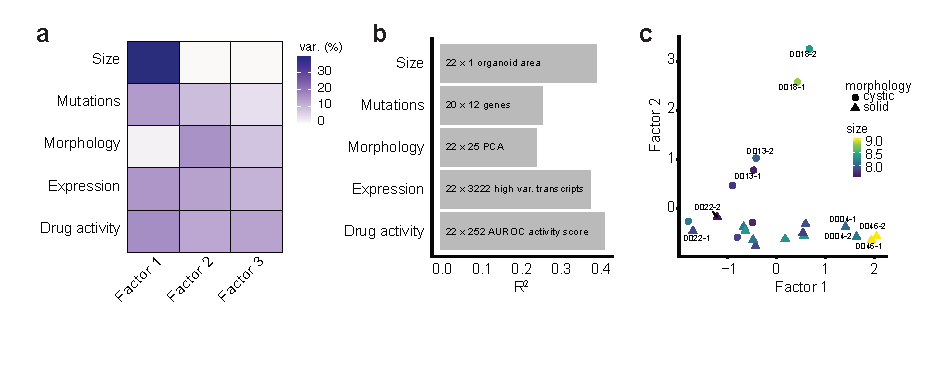
\includegraphics[width=\textwidth,
                height=\textheight,
                keepaspectratio]{figures/promise/pdf/fig_4_0.pdf}
\caption{}
\label{fig_240}
\end{figure}
\bigbreak

To learn a joint representation of unperturbed organoid morphology, unperturbed organoid size, gene expression, somatic mutations, and drug activity, multi-omics factor analysis (MOFA) was performed. MOFA is a matrix factorization method built upon group factor analysis, with decomposes a set of different measurements into a shared table of factors scoring each observed sample and a set of corresponding tables linking each factor to features in the set of original measurements. 

\bigbreak


\bigbreak
When trained with a low number of k = 3 factors, MOFA recovered factors explaining ca. 41-24\% of variance across the different data modalities, with the first two factors accounting for ca. 29-17\% in aggregate (Figure \ref{fig_240} a). While gene expression, mutations and drug activity profiles for organoid lines contributed to all factors, factor 1 captured an exceptional amount of variation in median organoid size (ca. 39\%). In contrast, factor 2 was primarily capturing variation within baseline organoid morphology (ca. 16\%) (Figure \ref{fig_240} a).

\bigbreak
Overall, MOFA factors explained up to 40\% of variance in median organoid size, drug activity and gene expression, while less than 30\% of variance in baseline organoid morphology was explained by the model (Figure \ref{fig_240} b). Organoid lines D046T and D004T stood out as lines with the strongest score for factor 1, while lines D018T and D013T had the strongest score in factor 2. Visual inspection of organoids revealed that organoid lines with a higher factor 1 score tended to be larger in size and organoids with high factor 2 score tended to have a more cystic organoid architecture based on manual classification (Figure \ref{fig_240} c). No interpretable morphological differences between factor 3 low and high organoids was identifiable, so the subsequent analysis was focused on the first two interpretable factors generated by MOFA. 

\bigbreak
To summarize, MOFA identified factors within the dataset that explained variation between organoid lines across different data modalities, including organoid morphology and median organoid size. 


\begin{figure}[h!]
\centering
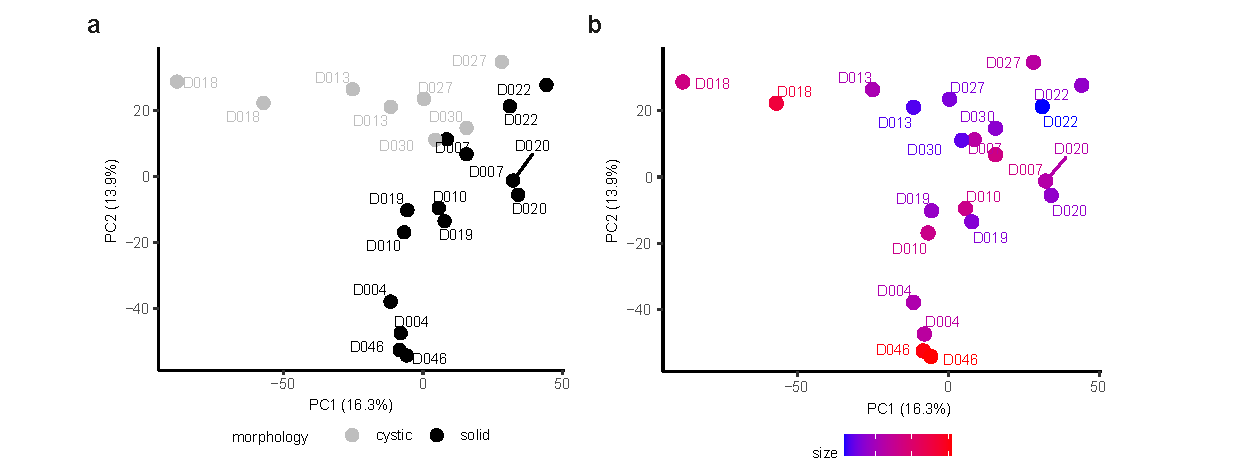
\includegraphics[width=\textwidth,
                height=\textheight,
                keepaspectratio]{figures/promise/pdf/fig_4_1.pdf}
\caption{}
\label{fig_241}
\end{figure}
\bigbreak

\begin{figure}[h!]
\centering
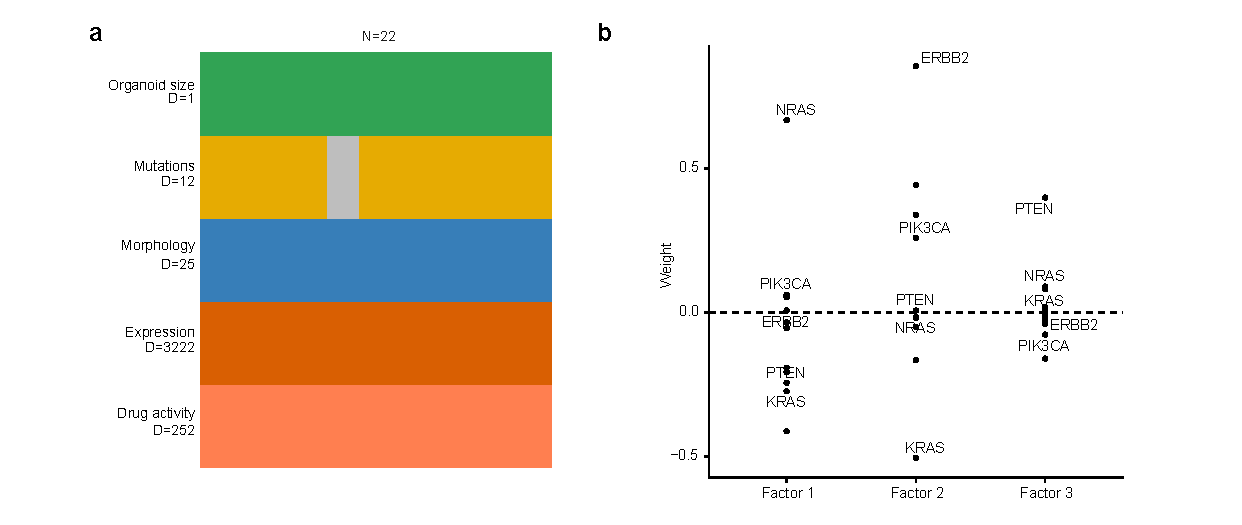
\includegraphics[width=\textwidth,
                height=\textheight,
                keepaspectratio]{figures/promise/pdf/fig_4_2.pdf}
\caption{}
\label{fig_242}
\end{figure}
\bigbreak


\section{An IGF1R signaling program is associated with increased organoid size, decreased EGFR inhibitor activity and can be induced by mTOR inhibition}

Differences in organoid size are an obvious contrubting factor to intra- and inter-organoid line heterogeneity. Organoid size was influenced by both organoid line and drug treatments and was associated with factor 1 scores (Fig 6a). An unsupervised gene set enrichment analysis (GSEA) for reactome pathways across factor 1 loadings showed an enrichment for IGF1R signaling and mitogen-activated protein kinase signaling related genes. In fact, the IGF signaling related transcripts H19 (rank 1) and IGF2 (rank 13) were among the strongest contributors to factor 1. This increase in proliferative signaling was confirmed by GSEA of a previously identified intestinal proliferation signature.31 To better understand clinical correlates to the identified gene expression patterns, we tested for molecular subtypes stemming from an analysis of cancer-cell intrinsic gene expression profiles.32 Factor 1 showed an enrichment for CRIS D, a molecular subtype linked to IGF2 overexpressing tumors with resistance to EGFR inhibitor therapy (Fig 6c), and a depletion for CRIS C, which has been linked to EGFR dependency (Supplemental Figure S8a). In fact, activity of EGFR inhibitors was the strongest contributor to a negative factor 1 score while IGF1R and MEK inhibitor activity contributed to a positive factor 1 score (Fig 6d-e, Supplemental Figure 8b-d).

\begin{figure}[h!]
\centering
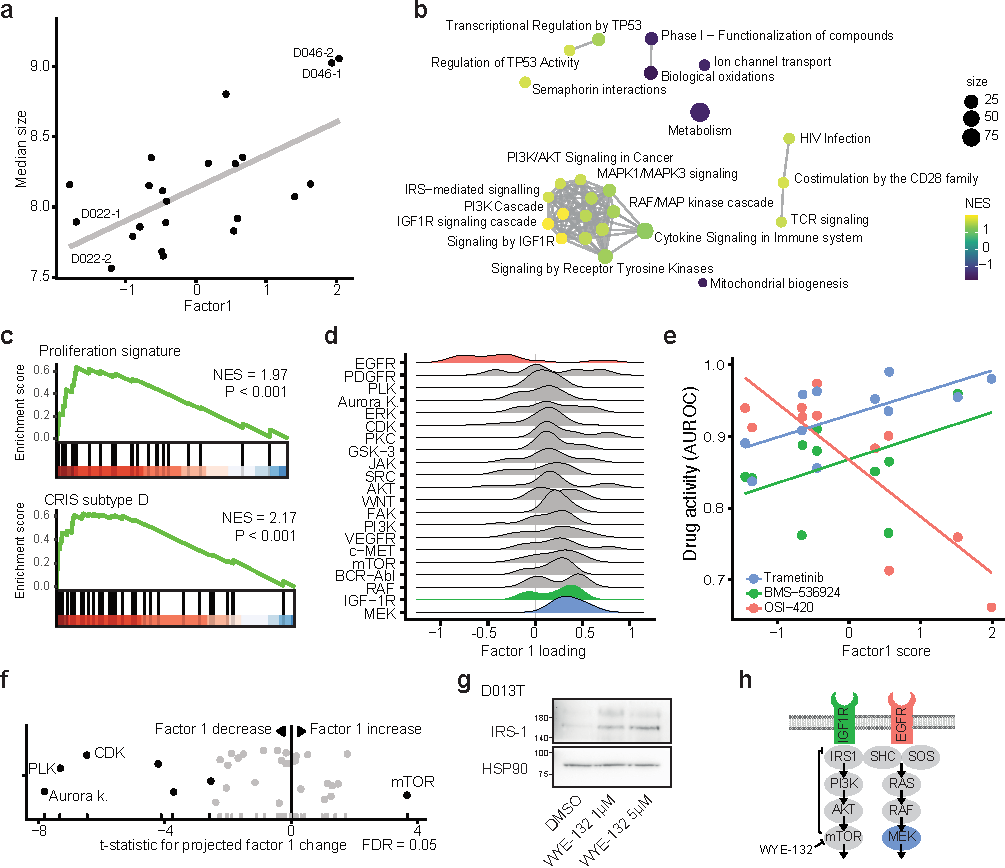
\includegraphics[width=\textwidth,
                height=\textheight,
                keepaspectratio]{figures/promise/pdf/fig_6_1.pdf}
\caption{}
\label{fig_261}
\end{figure}
\bigbreak

Prompted by the observation that mitogenic signaling, including IGF1R signaling, was underlying factor 1, we hypothesized that other compound treatments could influence the plasticity between the observed organoid states by modulating signaling pathway activity within organoids. To tested whether drug treatments shifted organoid phenotype profiles in factor space, I took advantage of the previous observation that unperturbed and certain perturbed organoids shared similar phenotypic profiles. To this end, the previously estimated factor loading matrix for unperturbed organoid morphology, which was generated during MOFA training, was used as a starting point. By generating the pseudoinverse of the loading matrix and multiplying with average phenotypic profiles of drug-treated organoids, the influence various drug treatments had on biological programs previously identified in unperturbed organoids was approximated. A group of cell cycle related kinase inhibitors targeting polo like kinases, Aurora kinases and cyclin dependent kinases shifted organoids to a low factor 1 score. In contrast, mTOR inhibitor treatment increased factor 1 scores in cancer organoids (Fig 6f and Supplemental Figure S8e). Given the observation that factor 1 was associated with IGF-1R signaling and mTOR inhibitor treatment led to an increase in factor 1 scores, I hypothesized that mTOR inhibition leads to a reactive upregulation of IGF1R signaling in cancer organoids. In fact, inhibition of mTOR signaling had previously been linked to transcriptional disinhibition of IRS-1 in a negative feedback loop33 and  reactive induction of IGF1R signaling had previously been described as a resistance mechanism to small molecule mTOR inhibitors in cancer.34 When testing this hypothesis in patient derived organoids, a dose-dependent increase of IRS-1 protein abundance in organoids treated with the ATP competitive mTOR inhibitor WYE-132 was observable (Fig 6g). To summarize, factor 1 described an organoid state with relatively large organoid size, elevated IGF1R dependent mitogenic signaling and relative inactivity of EGFR inhibitor treatment that could be induced by inhibiting an mTOR dependent negative feedback loop in patient derived cancer organoids.

\begin{figure}[h!]
\centering
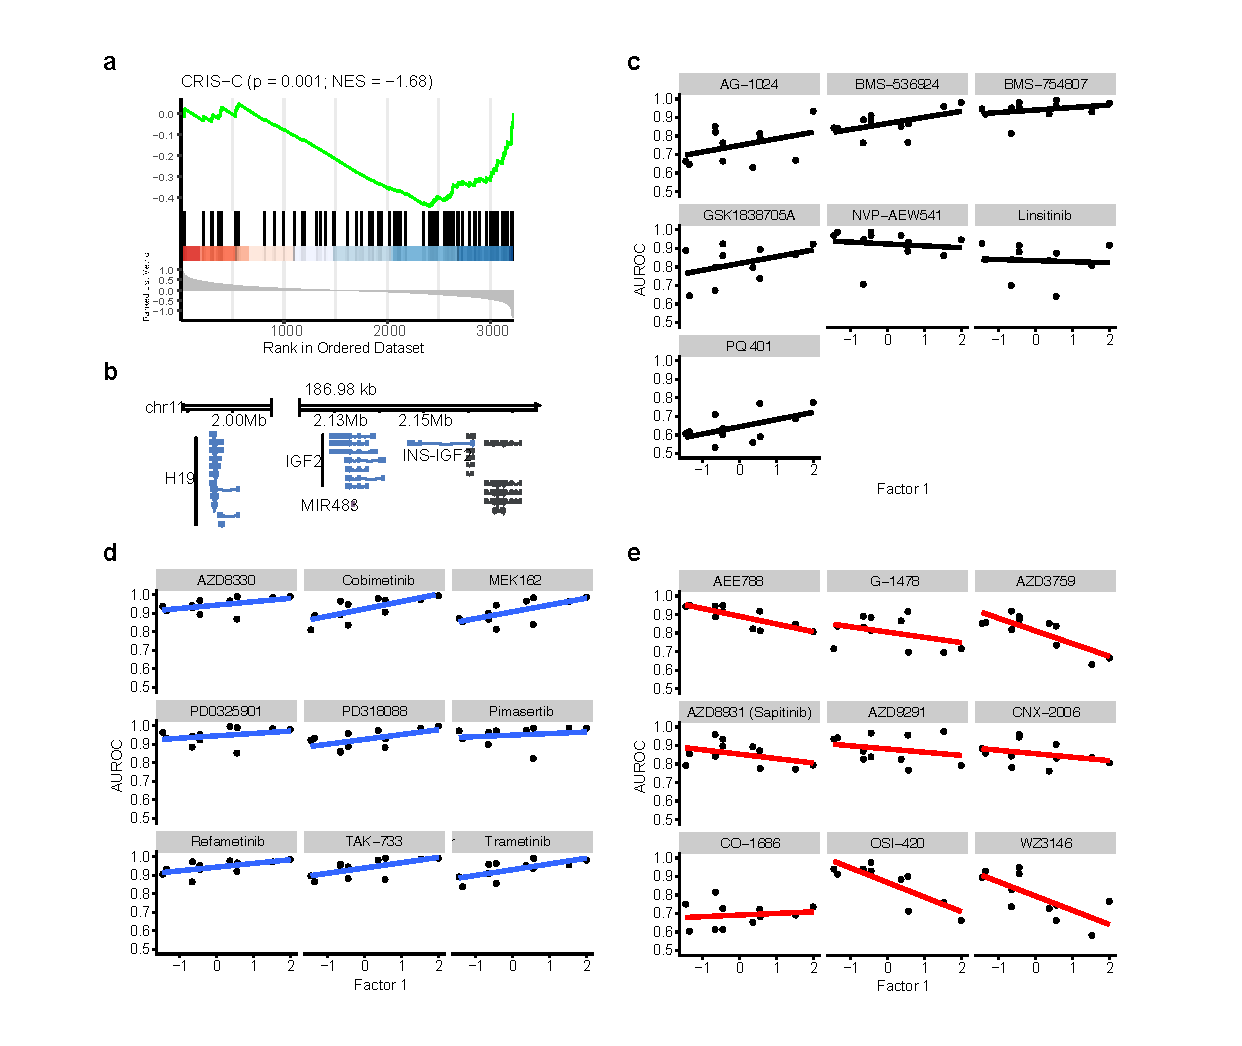
\includegraphics[width=\textwidth,
                height=\textheight,
                keepaspectratio]{figures/promise/pdf/fig_6_2.pdf}
\caption{}
\label{fig_262}
\end{figure}
\bigbreak



\section{An LGR5+ stemness program is associated with cystic organoid architecture and can be induced by inhibition of MEK}

A particularly strong recurring organoid phenotype was the presence of a cystic organoid architecture, seen in untreated D018T organoids and organoids treated with MEK inhibitors (Fig 1e, 3f, 5a). In the cystic state, which was observed in factor 2 high organoid lines, organoids consisted of a monolayer of uniform cells lining a central spherical lumen with a distinct apico-basally oriented actin cytoskeleton (Fig 5b). This phenotype was reminiscent of organoid morphologies previously seen in APC-/- or Wnt ligand treated human intestinal organoids. 

\begin{figure}[h!]
\centering
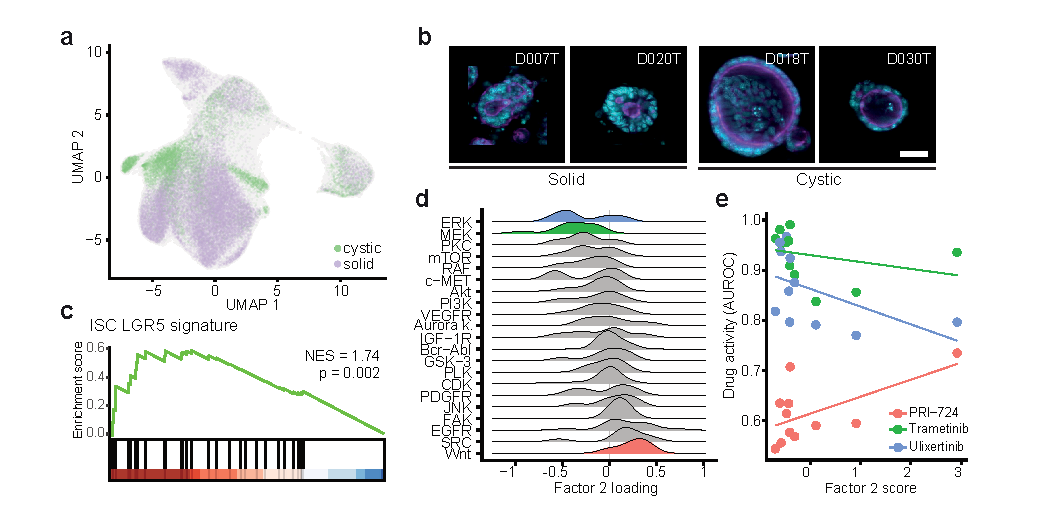
\includegraphics[width=\textwidth,
                height=\textheight,
                keepaspectratio]{figures/promise/pdf/fig_5_1.pdf}
\caption{}
\label{fig_251}
\end{figure}
\bigbreak

To test if factor 2 comprised Wnt signaling and intestinal stem cell identity related gene expression programs, gene set enrichment analyses (GSEA) was performed for cell identity signatures previously identified in intestinal crypts and colorectal cancer. GSEA revealed an enrichment of Lgr5+ stem cell signature-related genes for the factor 2 loadings (FDR=0.002, NES=1.74) (Fig 5c and Supplemental Figure S7a).31 Next, we wondered whether factor 2 was associated with particular drug activity or inactivity patterns. Activity of Wnt signaling inhibitors and EGFR inhibitors were the strongest average contributors to a positive factor 2 score (t statistic = 3.02, FDR = 0.046 and t statistic = 3.08, FDR = 0.046, respectively), while activity of ERK and MEK inhibitors were associated with a low factor 2 score (Fig 5d), albeit not significantly. As expected from these results, factor 2 high organoid lines showed a stronger morphological response to the Wnt pathway inhibitor PRI-724. (Fig 5e and Supplemental Figure S7b).




\begin{figure}[h!]
\centering
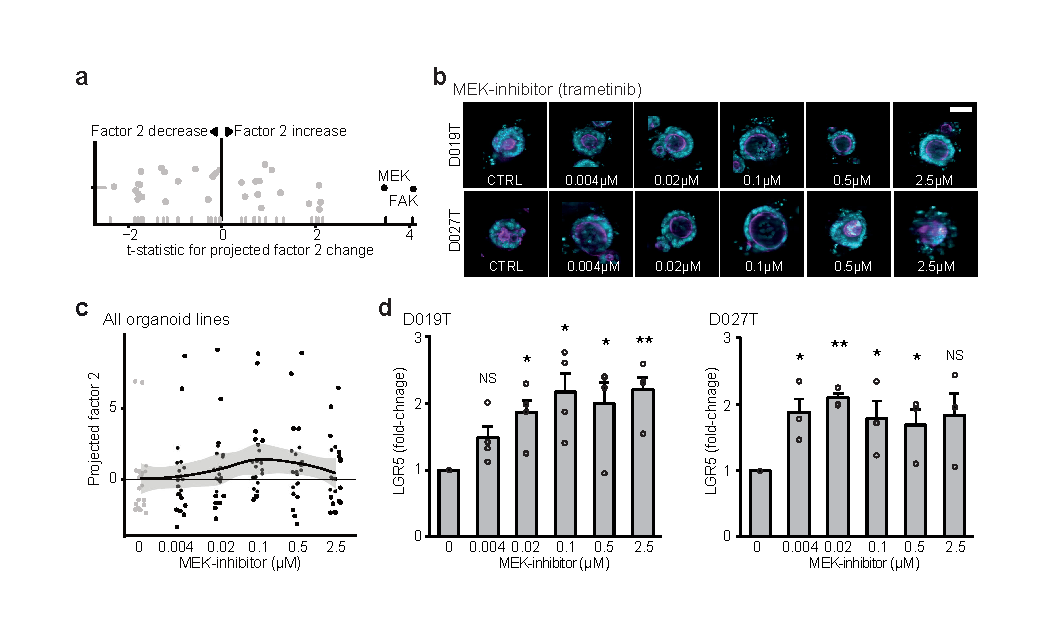
\includegraphics[width=\textwidth,
                height=\textheight,
                keepaspectratio]{figures/promise/pdf/fig_5_3.pdf}
\caption{}
\label{fig_253}
\end{figure}
\bigbreak

Next, we again used phenotype profiles of drug treated organoids and approximated how drug treatment shifted organoids along the factor 2 program. We observed MEK and focal adhesion kinase inhibitors significantly shifting all tested organoid lines towards higher factor 2 scores (Fig 5f and Supplemental Figure S7c). This change in factor 2 scores was concentration dependent for MEK inhibitors (Fig 5g and Supplemental Figure S7d-e) and coincided with a visual shift in organoid morphology (Fig 5h). Given the observation that factor 2 was enriched for an LGR5+ stem cell signature, we measured the expression of LGR5 transcripts at different concentrations of MEK inhibitor treatment and observed analogous dose-dependent increases in transcript abundance. In summary, factor 2 represents an organoid state with cystic architecture, increased expression of LGR5+ stem cell related genes and increased sensitivity to Wnt signaling inhibitors that could be induced by MEK inhibition.

\end{flushleft}
\begin{savequote}[75mm]
What I cannot create, I do not understand.
\qauthor{Richard Feynman}
\end{savequote}

% pending plagiarism check
\begin{flushleft}
\chapter{Profiling to identify revertant therapeutics in pre-malignant models of colon cancer}

\section{Motivation}

Based on the observation that (1) joint representations of organoid morphology and biological state can be learned, and (2) small molecule perturbations can shift organoids in representation space, the following hypothesis can be formulated: If well-annotated small molecules can help explain unknown organoid states, unknown small molecules with desirable properties should be identifyable by their ability to shift the state of well-annotated organoid models. 
Put differently, instead of using small-molecule perturbations to learn about the biology of non-characterized patient derived organoids, it should be possible to use genetically engineered organoid models to learn about desirable properties of non-characterized small molecules.
\smallbreak
To test this hypothesis, I generated a set of genetically engineered mouse colon organoid models that model the initiation of colorectal cancer via the chromosomal instability process \cite{Fearon1989-wf}. The emergence of colorectal cancer via the chromosomal instability process is a well understood sequence of genetic events that start with hyperactivation of canonical Wnt signaling, often via loss of APC, followed by the hyperactivation of RAS-MAPK signaling, often via oncogenic mutations of KRAS. These two mutations are frequent and signficantly co-occuring in colorectal cancer patients \cite{Schell2016-ew}, suggesting an interplay between these two acquired genetic functional events that lead to an evolutionary advantage of premalignant cells. While the genetic events within this process are well understood, no therapeutics targeting the loss of APC or the hyperactivation of KRAS via the frequent G12D activation have been developed for clinical use yet. 

\begin{figure}[h]
\centering
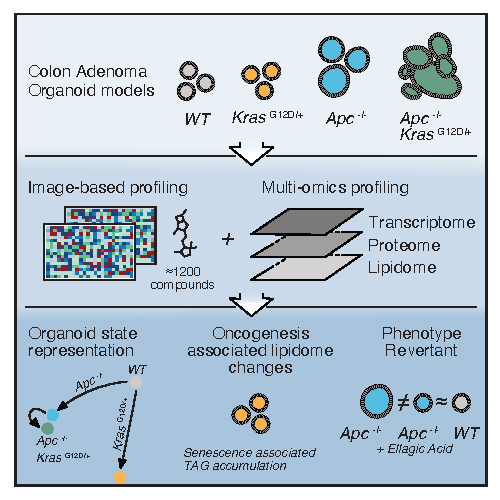
\includegraphics[width=250,
                height=\textheight,
                keepaspectratio]{figures/adenomaprofiling/pdf/fig_0_2.pdf}
\caption{\textbf{Visual abstract of adenoma model profiling project.} Mouse colon organoid models were developed, characterized and subjected to image-based small molecule profiling. The resulting data was used to learn a representation space of organoid states, identify state dependent changes in organoid lipid composition and generate hypotheses about small molcules that potentially have the ability to move organoid states.}
\label{fig_a02}
\end{figure}
\bigbreak

I genetically engineered mouse colon organoid models carrying Apc truncating mutations and/or a Kras G12D allele, thereby modelling the first set of genetic events within the chromosomal instability process leading to colorectal cancer. Using a strategy similar to the approach in the first chapter of this thesis, organoid models were characterized in-depth and subjected to a high-throughput small molecule screen of ca. 1700 FDA-approved substances and experimental compounds. The goal of this project was to (1) understand the biological state changes caused by individual transforming genetic changes in Apc and Kras within colon epithelial cells and (2) identify putative candidates that shift organoid states within the learned representation away from a transformed state. 


\begin{figure}[H]
\centering
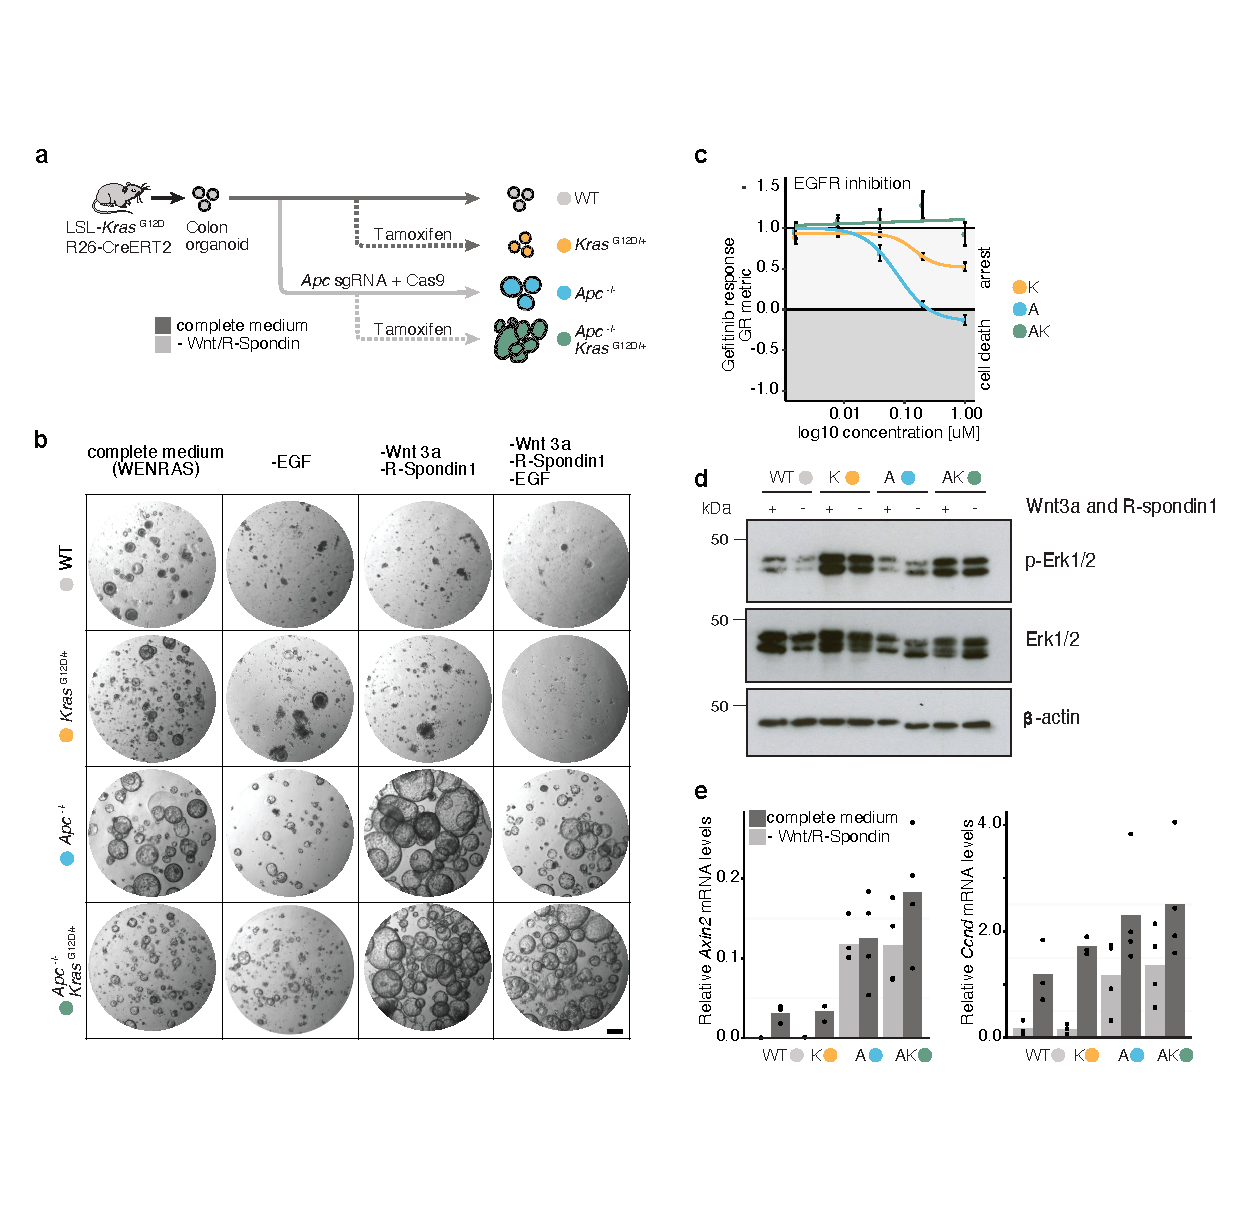
\includegraphics[width=\textwidth,
                height=\textheight,
                keepaspectratio]{figures/adenomaprofiling/pdf/fig_1_0.pdf}
\caption{\textbf{Establishing organoid models of colon adenoma, a} Overview of organoid model establishment. Mouse colon organoids were isolated from a transgenic donor animal carrying an inactive conditional oncogenic KrasG12D allele. Homozygous truncation of Apc via CRISPR and activation of the heterozygous KrasG12D allele lead to four different genetically defined organoid models.
\textbf{b} In vitro growth factor dependency of adenoma models. Organoids were cultured in complete or modified medium containing combinations of Wnt3A, R-Spondin1-Fc and EGF for 120h and subsequently imaged. Scalebar = 200µm.
\textbf{c}	Oncogenic KrasG12D increases resistance to Egfr inhibition. Organoid ATP levels were measured 4 days after Gefitinib treatment and adjusted for organoid growth rate. Points represent mean of n=2 independent experiments. Error bars represent standard error of mean.  
\textbf{d} Erk phosphorylation is increased by oncogenic KrasG12D. Organoid models were cultured with or without Wnt3A and R-Spondin1-Fc for 72h and analyzed for protein levels. p, phospho.   
\textbf{e}	Loss of Apc induces transcription of canonical Wnt-signaling target genes. qRT–PCR for Axin2 and Ccnd in the presence or absence of Wnt 3a and R-spondin1-Fc after 120h of culture. Expression levels are normalized to Sdha and Hprt transcript abundance. Bar graphs represent the mean of n=4 independent experiments.
}
\label{fig_a10}
\end{figure}
\bigbreak

\section{Generation of organoid colon adenoma models}
APC and KRAS mutant lesions are considered intermediate colon adenomas \cite{Fearon1989-wf}. To model the formation of colon adenomas in vitro, I used a transgenic mouse to derive organoid cultures. The transgenic animal carried a conditional tamoxifen inducible KrasG12D/+ allele \cite{Jackson2001-wv} (Figure \ref{fig_a10} a). After isolation, I confirmed that extracted colon organoids did not express an activated form of KrasG12D (Figure \ref{fig_a11}a) and defined these organoids as wildtype (WT). To model loss-of-function mutations of the tumor suppressor Apc, the frequently mutated mutation-cluster-region on the APC gene was targeted by CRISPR (Figure \ref{fig_a10} a). Generated organoids harbored biallelic loss-of-function mutations in Apc (Figure \ref{fig_a11}a). Subsequent activation of oncogenic KrasG12D by treatment with 4-Hydroxytamoxifen led to four distinct organoid adenoma models (Figure \ref{fig_a10} a and Figure \ref{fig_a11}a-b); wildtype (WT), Apc-/- (A), KrasG12D/+ (K), and Apc-/- / KrasG12D/+ (AK).


\begin{figure}[h]
\centering
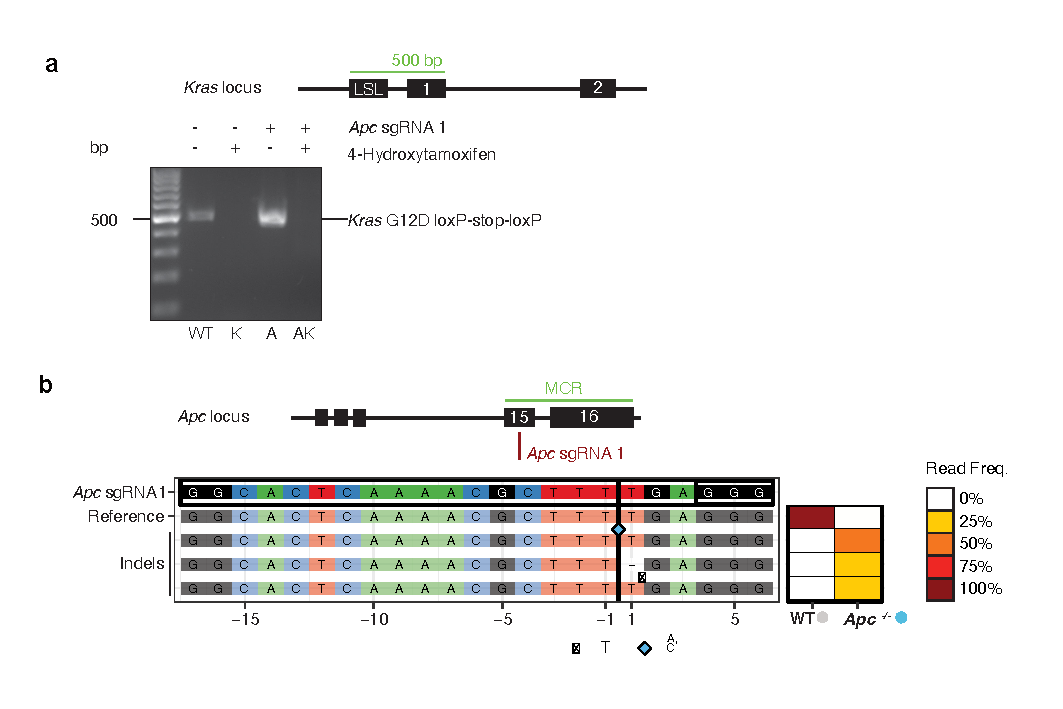
\includegraphics[width=\textwidth,
                height=\textheight,
                keepaspectratio]{figures/adenomaprofiling/pdf/fig_1_1.pdf}
\caption{\textbf{Structural validation of organoid colon adenoma models, a} Allele-specific PCR products of colon organoid models isolated from a transgenic mouse with a conditional tamoxifen inducible KrasG12D/+ allele.
\textbf{b} Amplicon sequencing result of the murine mutation cluster region ortholog for organoids transfected with an Apc targeting sgRNA and Cas9 carrying plasmid. The sequencing results show the presence of 3 different insertion/deletions within the pool of sgRNA treated organoid models. Wildtype sequences are absend within the CRISPR targeted pool, while mutant sequences are absent in the untreated organoid pool.}
\label{fig_a11}
\end{figure}
\bigbreak

Similar to genetically modified human colon organoids \cite{Drost2015-ph, Matano2015-zw}, adenoma models showed characteristic niche requirements. Both Apc mutant organoid lines grew independent of the Wnt-signaling activating factors Wnt 3a and R-Spondin1 (Figure \ref{fig_a10} b). In fact, Apc mutant lines showed an increased growth in a Wnt3a and R-Spondin1 free environment when compared to the complete medium. 

\smallbreak
Organoid models with an activated KrasG12D allele were less sensitive to removal of EGF from the media. However, as observed before \cite{Drost2015-ph}, the mutant KrasG12D allele was insufficient to compensate completely for the loss of EGF from the medium. Nevertheless, KrasG12D mutant organoid lines were more resistant to pharmacological inhibition of Egfr signaling (Figure \ref{fig_a10} c). In conclusion, organoid model genotypes were reflected in characteristic growth factor dependencies.

\smallbreak
Next, I investigated the effects of mutations in Apc and Kras on both canonical Wnt- and Erk dependent signaling. While the presence of the KrasG12D/+ allele led to an increase in Erk-phosphorylation across models, Apc-/- / KrasG12D/+ organoids showed no marked additional increase in Erk-phosphorylation when compared to KrasG12D/+ organoids (Figure \ref{fig_a10} d). Moreover, Apc-/- / KrasG12D/+ adenoma models showed no significant differences in expression of the Wnt target genes Axin2 and Ccnd when compared to Apc-/- single-mutant models (A) (p > 0.34 for all conditions, Wilcoxon rank sum test) (Figure \ref{fig_a10} e). These results indicate that organoid adenoma models show genotype-dependent activity of characteristic signaling pathways, while there is no extensive crosstalk between the Apc-/-  and KrasG12D/+ allele in mouse colon organoids that that is directly reflected in canonical Wnt- and Erk dependent signaling.  

\bigbreak
\section{Biochemical profiling of organoid models}
To explore comprehensive molecular differences between organoid models, I next performed transcriptome, proteome and lipidome profiling of all four organoid models (Figure \ref{fig_160}). Transcriptome profiling of organoid models showed an increased expression of the stem-cell marker Lgr5 and Wnt-signaling regulators such as Nkd1, Notum, Wif1 and Znrf3 in Apc mutant organoid lines (Figure \ref{fig_160} b). To the contrary, Apc wildtype organoid lines showed an increased expression of epithelial differentiation markers, such as Krt20, Alpp and Abcb1 (P-glycoprotein). Overall, the number of genes with significant expression changes after Apc loss was 2.5 times greater compared to isolated KrasG12D activation (FDR = 0.1, Apc-/-: 44.5\%, KrasG12D/+: 18.3\% of assessed genes). 

\begin{figure}[H]
\centering
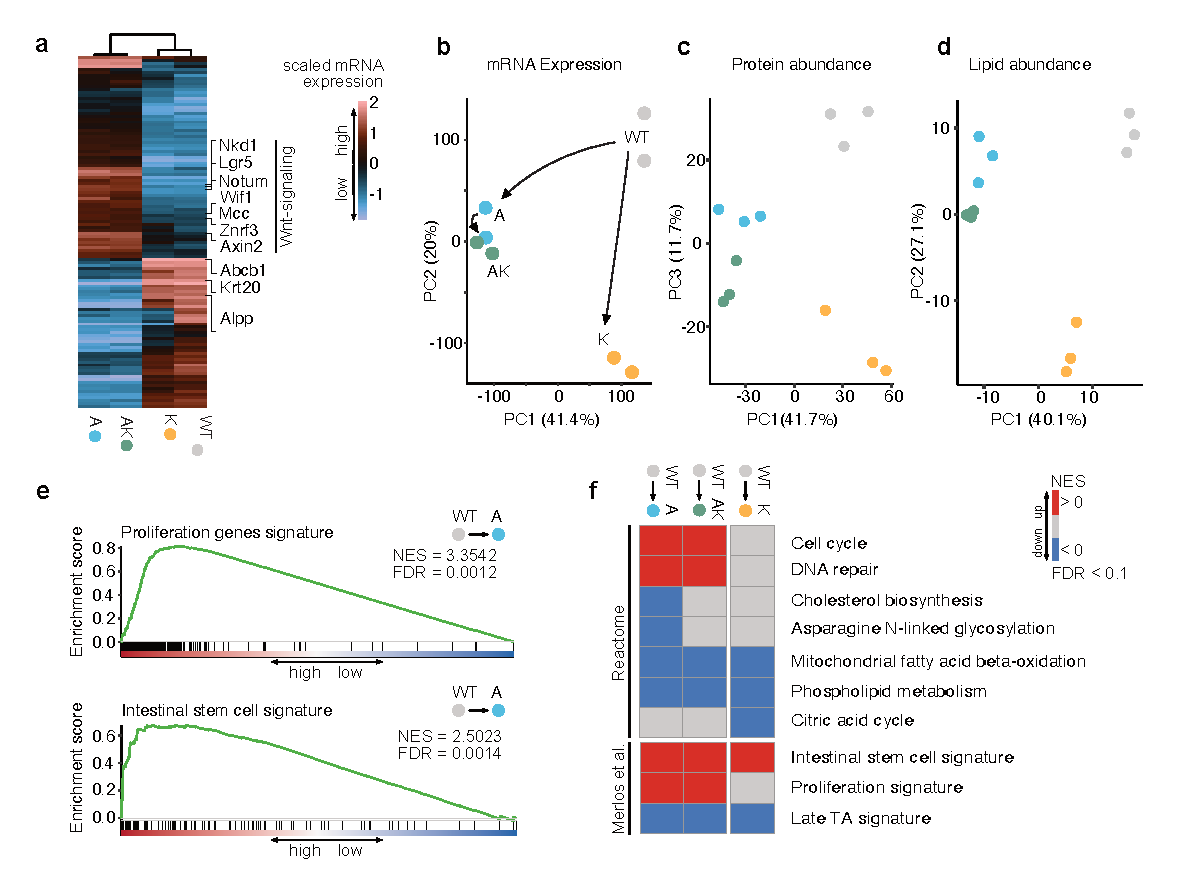
\includegraphics[width=\textwidth,
                height=\textheight,
                keepaspectratio]{figures/adenomaprofiling/pdf/fig_1_6_1.pdf}
\caption{\textbf{Molecular profiling of organoid adenoma models. a} Differential gene expression of adenoma models. Shown are scaled expression values for the top 125 differentially expressed genes for every organoid line. Selected genes are highlighted. All organoids were cultured for 3 days in WENRAS before exposure to ENR for 4 days. Cell number was controlled between experiments. Whole organoid lysates were analyzed. 
\textbf{b} Transcript abundance data. Shown are the first two principal components of scaled gene expression data. The proportion of variance of each principal component is listed in parenthesis. 
\textbf{c} Protein abundance data. Shown are the first and third principal component of scaled protein expression data. The proportion of variance of each principal component is listed in parenthesis. 
\textbf{d} Lipid species abundance data. Shown are the first two principal components of scaled lipid abundance data. The proportion of variance of each principal component is listed in parenthesis. 
\textbf{e} Loss of Apc leads to increased expression of proliferation and intestinal stem cell associated genes. Shown is a gene set enrichment analysis of differentially expressed genes between Apc mutant and WT organoids. Intestinal gene expression signatures were used according to Merlos-Suarez et al. NES, normalized enrichment score. 
\textbf{f} Overview of cellular processes in organoid adenoma models. Shown are selected enriched differential gene expression signatures from Reactome and Merlos-Suarez et al. NES, normalized enrichment score. NES > 0 suggests an enriched/ activated biological process. FDR < 0.1.}
\label{fig_161}
\end{figure}
\bigbreak

A related observation was made during the analysis of protein abundance. Proteome profiling and imputation identified 3906 gene products in all measured organoid lines. Again, Wnt signaling regulators (Axin2, Notum) were enriched in Apc mutant organoid lines and the number of significantly regulated proteins after Apc loss was 2.5 times greater compared to an isolated KrasG12D activation (FDR = 0.1, Apc-/-: 260, KrasG12D/+: 105 assessed proteins). 

\smallbreak
Principal component analysis of both transcriptome, proteome and lipidome data showed related axes of variation across measurements. In all observerd modalities, the first principal component captured differences between Apc wildtype and Apc mutant organoid models, while the second (in case of proteomics measurements the third) principal component captured differences between wildtype and KrasG12D/+ single-mutant models (Figure \ref{fig_161}b, \ref{fig_161}c and \ref{fig_161}d). In every modality, a high degree of similarity was observed among Apc-/- and Apc-/- / KrasG12D/+ organoid lines. While activation of oncogenic KrasG12D in wildtype organoids led to global changes in transcript, protein and lipid expression, these changes were not as pronounced in organoids without functional Apc. In fact, only the mRNA expression of 91 genes was significantly altered between Apc-/- and Apc-/- / KrasG12D/+ organoids (FDR = 0.1). 

\smallbreak
To explore activated biological processes, gene set enrichment analysis on organoid mRNA expression data was performed. The strongest changes in gene expression after loss of Apc were linked to an increased proliferative activity (Figure \ref{fig_160} e). Gene set enrichment analysis of published intestinal cell-proliferation and stem cell signatures showed an enrichment of both signatures in Apc-/- organoids (Figure \ref{fig_160} e) \cite{Merlos-Suarez2011-gd}. In contrast, a signature for differentiating, transit-amplifying cells was depleted. Gene set enrichment analysis of Apc-/- / KrasG12D/+ double-mutant organoids showed the same results. 

 \begin{figure}[h]
\centering
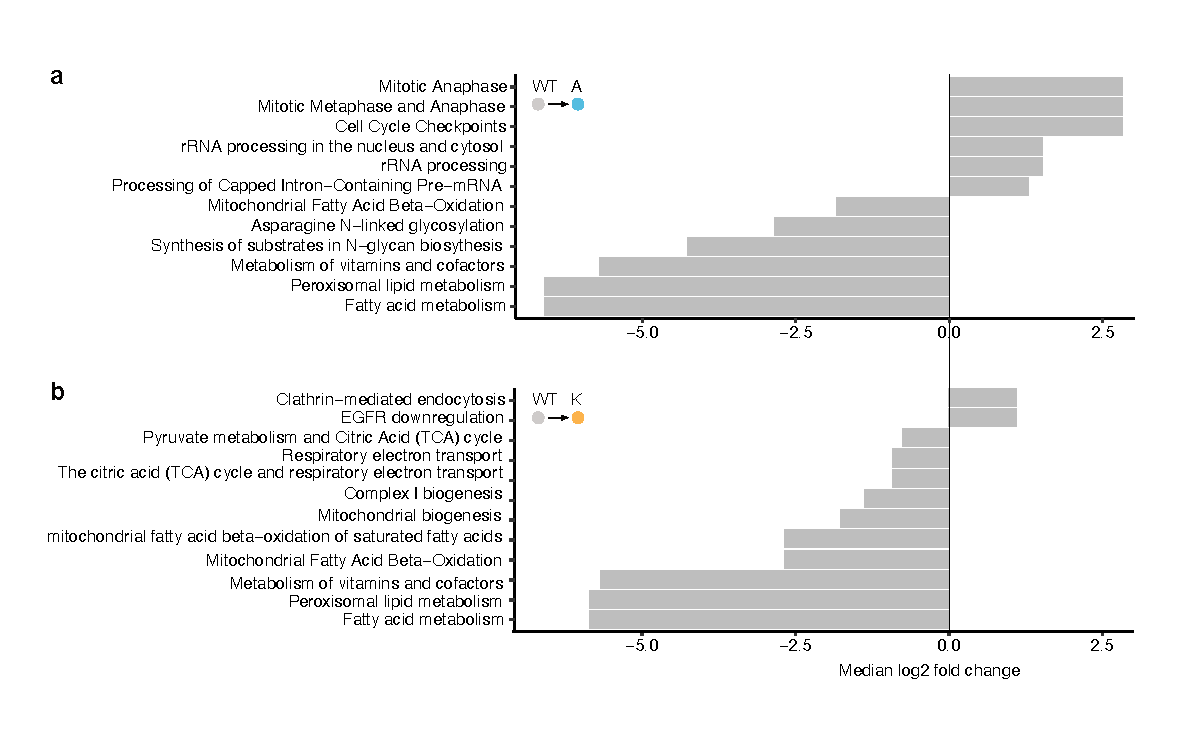
\includegraphics[width=\textwidth,
                height=\textheight,
                keepaspectratio]{figures/adenomaprofiling/pdf/fig_1_6_2.pdf}
\caption{
\textbf{a} Representative up and down-regulated transcriptional processes after loss of Apc. Expression signatures were sourced from Reactome and average log2 fold changes for included transcripts are illustrated. FDR < 0.1.
\textbf{b} Representative up and down-regulated transcriptional processes after activation of oncogenic Kras G12D. Expression signatures were sourced from Reactome and average log2 fold changes for included transcripts are shown. FDR < 0.1.
}
\label{fig_162}
\end{figure}
\bigbreak


Next to these published signatures, I explored the enrichment of curated gene sets from the Reactome database \cite{Griss2020-qi}. Here, both Apc-/- and Apc-/- / KrasG12D/+ double-mutant lines showed a positive enrichment of cell cycle and DNA repair related genes when compared to wildtype organoids (Figure \ref{fig_162}a). Unique to the KrasG12D/+ organoid line was a decreased expression of citric acid cycle and respiratory chain related genes (Figure \ref{fig_162}b). This effect, was not observed in Apc-/- / KrasG12D/+ double mutant organoids (Figure \ref{fig_161}f). In addition, organoid models with an KrasG12D/+ genotype showed a downregulation of the EGFR receptor, in line with a potential negative feedback response to hyperactivated RAS-MAPK signaling (Figure \ref{fig_162}b). Both Apc-/- and KrasG12D/+ organoid models showed a strong reduction of lipid metabolism and beta-oxidation (Figure \ref{fig_162}a,b).

\smallbreak
In summary, loss of Apc leads to a global shift in transcript, protein, and lipid abundance in colon organoids, including a strong increase in cell proliferation associated genes. Activation of isolated oncogenic KrasG12D leads to pronounced reduction in citric acid cycle related gene expression while this phenotype was not seen in organoid models with an additional loss of Apc.

\begin{figure}[h!]
\centering
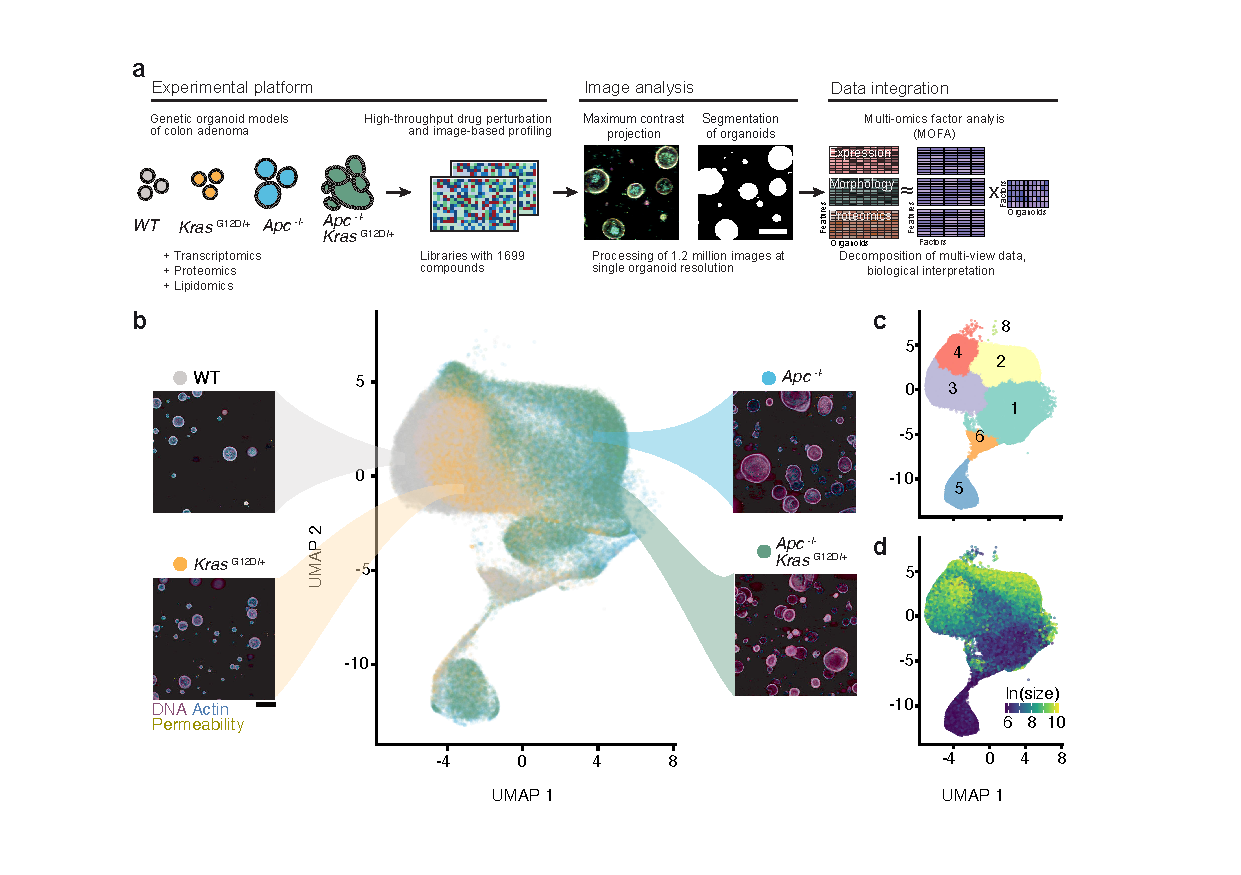
\includegraphics[width=\textwidth,
                height=\textheight,
                keepaspectratio]{figures/adenomaprofiling/pdf/fig_1_2.pdf}
\caption{\textbf{Image-based profiling of organoid adenoma models. a} Overview of experiments. Organoids were isolated from a transgenic mouse model and genetically edited. Organoids were dissociated and evenly seeded in 384-well plates before perturbation with an experimental small molecule library. After treatment, high-throughput fluorescence microscopy was used to capture the morphology of organoids in 16 selected z-layers and 3 channels. 3D imaging data were projected on a 2D plane using a maximum contrast projection. Here, only pixel areas with the largest contrast among the z-axis were retained. Morphological features were computed based on the projection. Untreated organoid morphology, organoid size and drug activity scores were integrated with transcript expression, protein abundance, lipid abundance and genogtype data in a Multi-Omics Factor Analysis (MOFA) model. Figure created with support from Johannes Betge (graphical presentation). 
\textbf{b} Uniform Manifold Approximation and Projection (UMAP) of organoid-level features for a random 5\% sample out of imaged organoids. The identical sample is used for visualizations throughout the figure. Organoid genotype is colorcoded and representative images are displayed (magenta = DNA, cyan = actin, cell permeability = yellow, scale-bar: 200µm). \textbf{c} Graph-based clustering of organoids by morphology with 8 resulting clusters. \textbf{d} Organoid size distribution. Color corresponds to the log-scaled organoid area (dark blue: minimum size, yellow: maximum size).}
\label{fig_120}
\end{figure}
\bigbreak

\newpage
\section{Image-based profiling of organoid models}

To measure how organoids change their biological state as a response to small molecule perturbation, I used the previously developed image-based profiling method to observe organoid morphology. Organoid models of four different genotypes were perturbed with a library of ca. 1700 compounds and morphological profiles were computed (Figure \ref{fig_120} a). A UMAP projection of 25 principal components representing single-organoid morphology showed distinct genotype-dependent morphological states for viable organoids (Figure \ref{fig_120} b). Graph based clustering of organoid morphology profiles resulted in 8 different clusters (Figure \ref{fig_120} c). While developed organoids within cluster 4 and 3 were enriched for Apc+/+ organoid models, cluster 2 and 1 were populated by Apc-/- models. Analogous to gene expression, lipidomics and proteomics representation space, Apc mutant organoid models were less distinct from each other than organoids with a WT and isolated KrasG12D/+ genotype (Figure \ref{fig_140} b). While developed organoids that present with a larger organoid area showed distinct genotype-specific morphologies, small and dead organoids clustered together across genotypes within cluster 5 (Figure \ref{fig_120} c and d). 

\bigbreak
\begin{figure}[h!]
\centering
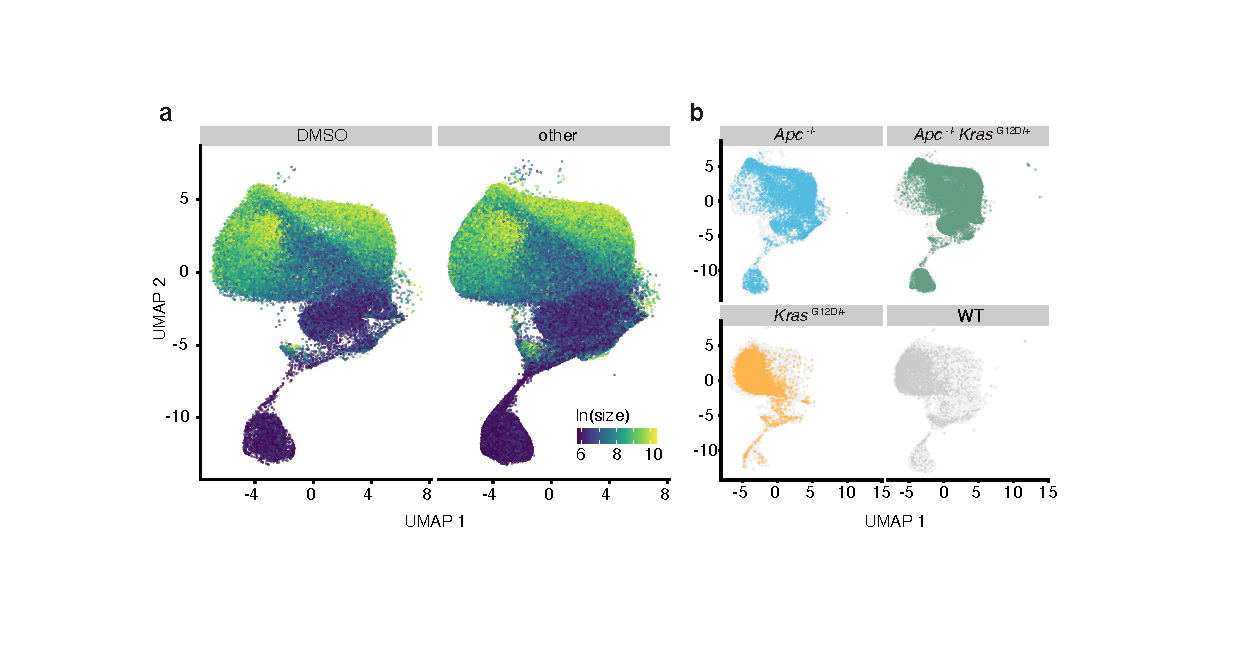
\includegraphics[width=\textwidth,
                height=\textheight,
                keepaspectratio]{figures/adenomaprofiling/pdf/fig_1_4.pdf}
\caption{\textbf{Treatment and genotype dependent effects on organoid morphology distribution. a} UMAP representation of DMSO treated (vehicle) and small molecule treated organoids. \textbf{b}, UMAP embeddings of four organoid genotypes (baseline state = 0.1\% DMSO control-treated organoids), grey background consists of randomly sampled organoids.}
\label{fig_140}
\end{figure}

The distribution of DMSO-treated organoids and small molecule perturbed organoids in morphological space overlapped strongly (Figure \ref{fig_140} a), possibly because of large amount of treatments that did not alter organoid morphology.

\begin{figure}[h!]
\centering
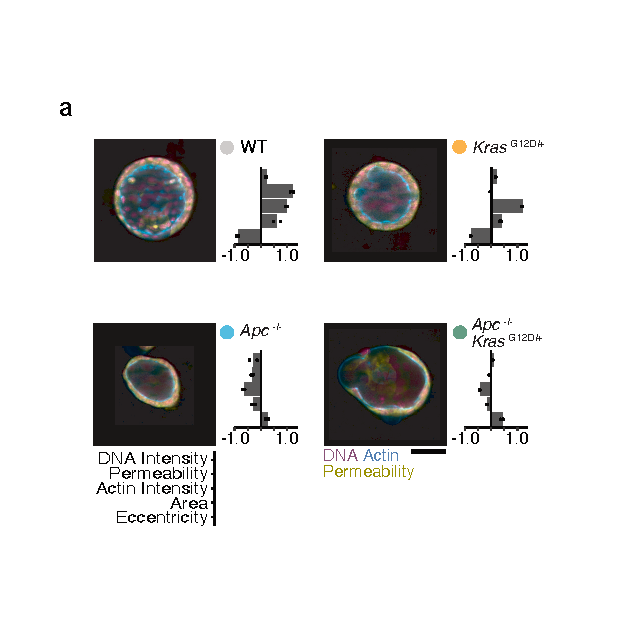
\includegraphics[width=200,
                height=\textheight,
                keepaspectratio]{figures/adenomaprofiling/pdf/fig_1_3.pdf}
\caption{\textbf{Genotype dependent effects on organoid morphology. a} Unperturbed organoid profiles from adenoma models were aggregated. Shown are representative individual organoids with selected features. Points show the mean phenotype for each independent biological replicate. Selected features and their z-scores relative to all single organoid profiles are shown (magenta = DNA, cyan = actin, cell permeability = yellow, scale-bar: 25µm)}
\label{fig_130}
\end{figure}
\bigbreak

When comparing the morphologies of different organoid models in detail, characteristic differences were identifiable (Figure \ref{fig_130} a). DMSO-treated Apc+/+ organoids showed a strong, regular apical actin cytoskeleton (high average actin intensity) that organized the multicellular formation into a regular-patterned spherical morphology (low average eccentricity). In contrast, Apc-/- organoids showed a relative lack of a regular actin cytoskeleton (low average actin intensity) and a irregular, non-spherical morphology (high average eccentricity). 

\smallbreak
In summary, developed organoids showed genotype-dependent differences in morphology. Analogous to differences in biochemical state, a primary source of variation was the loss of the tumor suppressor gene Apc. Organoids with truncated Apc presented with a loss of the spherical, potentially structure-conferring, and cell-spanning apical actin cytoskeleton that was observed in Apc +/+ organoid models.

\section{Quantifying small molecule induced phenotypes across organoid models}

\begin{figure}[h!]
\centering
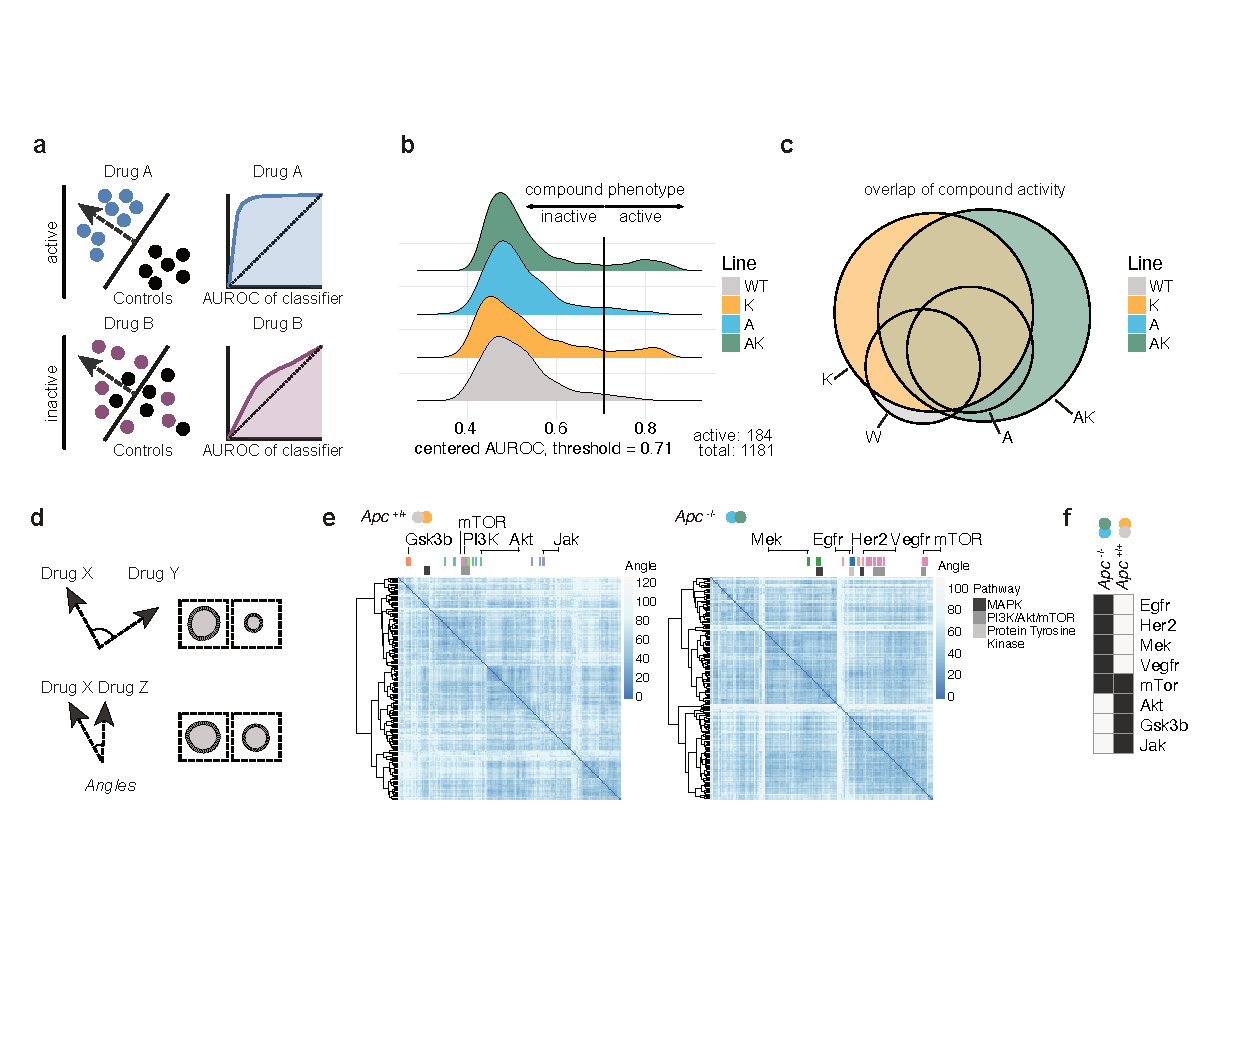
\includegraphics[width=\textwidth,
                height=\textheight,
                keepaspectratio]{figures/adenomaprofiling/pdf/fig_1_5.pdf}
\caption{\textbf{Small molecule activity scoring. a} A logistic regression classifier is trained to distinguish morphology profiles of individual treated and untreated organoids across all available replicates. Afterwards, the classifier is applied to a validation set of organoids and the classification performance is estimated using the area under the receiver operating characteristic curve (AUROC) metric. Method implemented by Jan Sauer.
\textbf{b} Distribution of AUROC compound activity scores for all organoid lines, replicates and perturbations. AUROC scores were centered around 0.5 and treatments for this particular analysis were termed active when classification accuracy exceeded three times the Median Absolute Deviation (MAD) of the AUROC score distribution, an arbitrary threshold. A set of 184 compounds (16\% of all screened small molecules) met the activity criteria. 
\textbf{c} Overlap of active compound treatments across organoid models. Shown is a Euler diagram of active compounds for each line. Apc -/- (abbreviated A), double mutant (Apc-/- KrasG12D+/-, abbreviated AK), Kras G12D (abbreviated K), and wildtype (abbreviated WT) are color coded. Plot diagnostics: diagError: 0.011, stress: 0.002.
\textbf{d} Identifying related treatment induced phenotypes. Normal vectors of treatment specific classifiers were compared by calculating the angular distance (related to cosine similarity, ranging from 0-180 degrees). Small angular distance between vectors correspond to a high similarity between the treatment-induced organoid phenotypes. Method implemented by Jan Sauer.
\textbf{e} A map of compound induced phenotypes for Apc mutant and Apc wildtype organoids. Highlighted are clusters of compound induced phenotypes with related targets. Normal vectors for Apc mutant and Apc wildtype organoids were concatenated before angular distance calculation. Method implemented by Jan Sauer.
\textbf{f} Treatment induced phenotypes by organoid genotype. Shown are significantly enriched treatment induced phenotypes for Apc mutant and wildtype organoid models. Clusters of similar phenotypes were tested for overrepresentation of known molecular targets using Fisher’s exact test. Significantly enriched targets are shown. Method implemented by Jan Sauer.
}
\label{fig_150}
\end{figure}
\bigbreak

To study the effect that small molecule perturbations had on organoid models, the classification based approach developed during the study of human cancer organoid phenotypes in the previous chapter was used. Briefly, for every treatment and genotype, a linear classifier was trained to distinguish DMSO-treated organoids from treated organoids. The classification performance, expressed as the AUROC obtained on a hold-out dataset, was used to determine the activity of a compound. A high AUROC (approaching 1) is observed for compounds that lead to a treatment-induced organoid morphology that is very distinct from DMSO treated organoids. In contrast a low AUROC (minimum of 0.5) is observed for compounds where the classification performance approaches random guessing (Figure \ref{fig_150} a).

\smallbreak
Related to the approach chosen in the previous chapter, active treatments were identified based on the AUROC score that a classifier reached. Given differences in the distribution of AUROC scores between lines, with KRAS G12D/+ organoid lines being shifted towards higher AUROC values, I centered the distribution of AUROC scores around 0.5 and defined an arbitrary activity threshold at 3 times the Median Adjusted Deviation for all tested models (Figure \ref{fig_150} b). A primary source of variation in the genotype-dependent identity of active compounds (16\% of all tested small molecules) was the functional state of Apc, as most active compounds were shared among Apc+/+ and Apc-/- models, while little relative overlap existed between these two alleles (Figure \ref{fig_150} c). As described above, the higher classification performance seen in organoids with the Kras G12D/+ allele, led to a larger number of active drugs identified for these models. A possible reason for this systematic difference in the number of active treatments might be a larger number of organoids seen in the images of these models. This difference might be linked to the previously described increased colony-forming capacity seen in Kras G12D/+ colon cancer models \cite{Patankar2019-ee}.

\smallbreak
Given the observation that the primary source of variation for drug activity, similar to other biochemical assays, was the state of the Apc allele, I focused the analysis of treatment-induced organoid phenotypes along this axes. Similar to the approach taken in the previous chapter, normal vectors of the logistic regression classifiers were compared by estimating the enclosed angle (Figure \ref{fig_150} d). Normal vectors for organoids with the same Apc allele were concatenated. The resulting clustering of normal vectors by their similarity showed an enrichment for small molecules with related mechanism of action (Figure \ref{fig_150} e and f). For example, EGFR inhibitors were significantly enriched in Apc-mutant organoid lines, while GSK3B-inhibitors, which lead to a stimulation of canonical Wnt signaling, were enriched in Apc-wildtype organoid models, only. 

\section{Multi-omics factor analysis identifies shared factors linking functional and structural biological views}

\begin{figure}[h!]
\centering
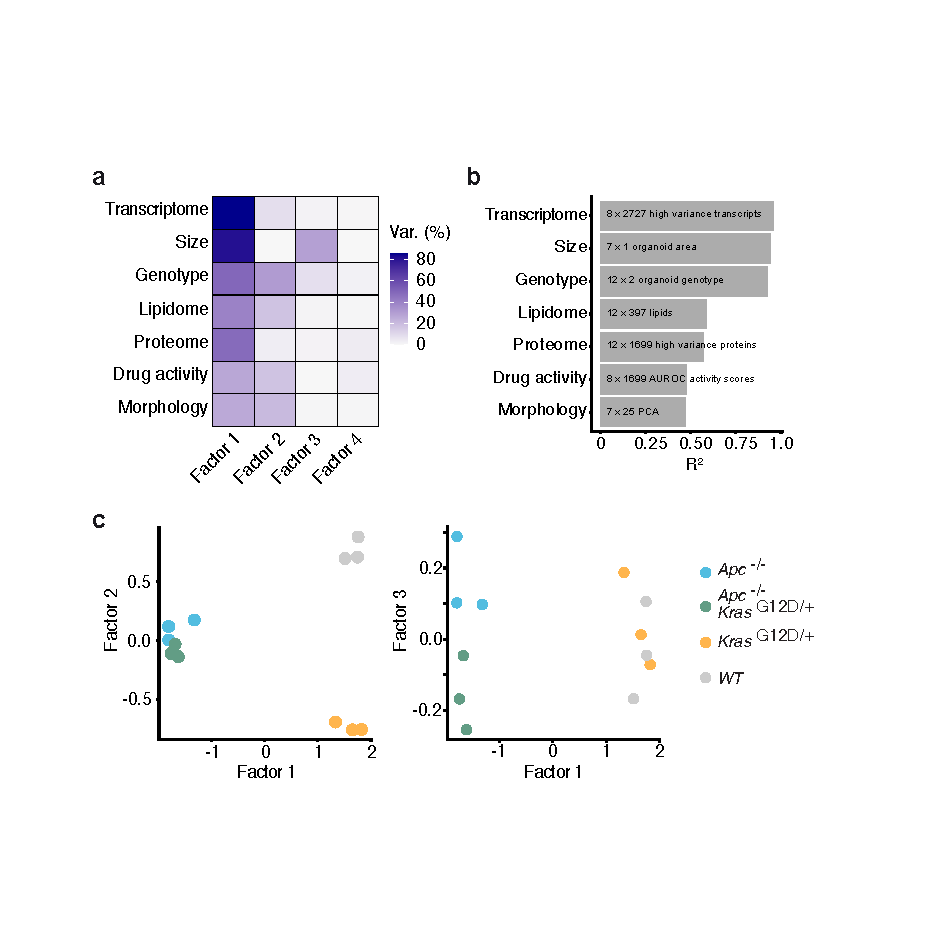
\includegraphics[width=350,
                height=\textheight,
                keepaspectratio]{figures/adenomaprofiling/pdf/fig_1_7.pdf}
\caption{\textbf{Multi-omics factor analysis to identify shared factors linking morphology, size, gene expression, lipidomics, proteomics, genotype and drug activity. a} Percent variance explained by the MOFA model for each factor. Untreated organoid morphology, organoid size and drug activity scores were integrated with genotype, proteomics, lipidomics and mRNA expression data. \textbf{b} Cumulative proportion of total variance explained by each experimental data modality within the MOFA model. \textbf{c}, Visualization of samples in factor space showing factors 1 and 2 as well as factor 1 and 3. Shown are independent replicates for each organoid line. 
}
\label{fig_170}
\end{figure}
\bigbreak

To comprehensively model the biological state of organoid models and explore potential interventions that move organoids in state-space, I performed multi-omics factor analysis (MOFA). Analogous to the process described in the previous chapter, feature matrices from different sources were processed and factorized using k=4 factors (Figure \ref{fig_170} a and \ref{fig_180} a). The learned model was based on both functional (e.g. drug activity) and structural (e.g. genotype, proteomics, lipidomics and mRNA expression) information. To reduce the dimensionality of input data, only high variance features from gene expression and proteomics analysis were used.

\smallbreak
The resulting factorization explained ca. 90\% (gene expression) to 50\% (morphology) of variance across the analyzed views, of which the first three factors captured the majority of variance, Figure \ref{fig_170} a). The learned model explained most variance within the mRNA expression and genotype data, while measurements within the organoid morphology data had the lowest explained variance (Figure \ref{fig_170} b). Visual inspection of factors as well as exploration of factor loadings within the genotype view showed that factor 1 explained state differences caused by Apc loss of function, while factor 2 explained state differences caused by the activation of KrasG12D in an Apc+/+ genotype (Figure \ref{fig_170} c and \ref{fig_180} b). In contrast to factor 2, factor 3 captured differences between Kras+/+ and KrasG12D/+ organoids with Apc loss of function, albeit with low overall explained variance. 

\smallbreak
While the initial number of factors is a user-defined feature within MOFA, the method automatically drops excess factors if they are not considered effective based on an applied automatic relevance determination (ARD) prior. Increasing the number of factors above k=4 in this analysis, did not lead to an increased number of interpretable factors. In fact, factor 4 already did not capture differences between organoid genoypes and was not interpretable from a biological point of view (Figure \ref{fig_180} b). This observation and the fact that this study explored the biological effects of two oncogenic genetic events both in isolation and in concert reveals, I speculate, a conceptual intersection of representation learning  and the theory of genetic interactions which will not be further explored in this thesis. 

\begin{figure}[h!]
\centering
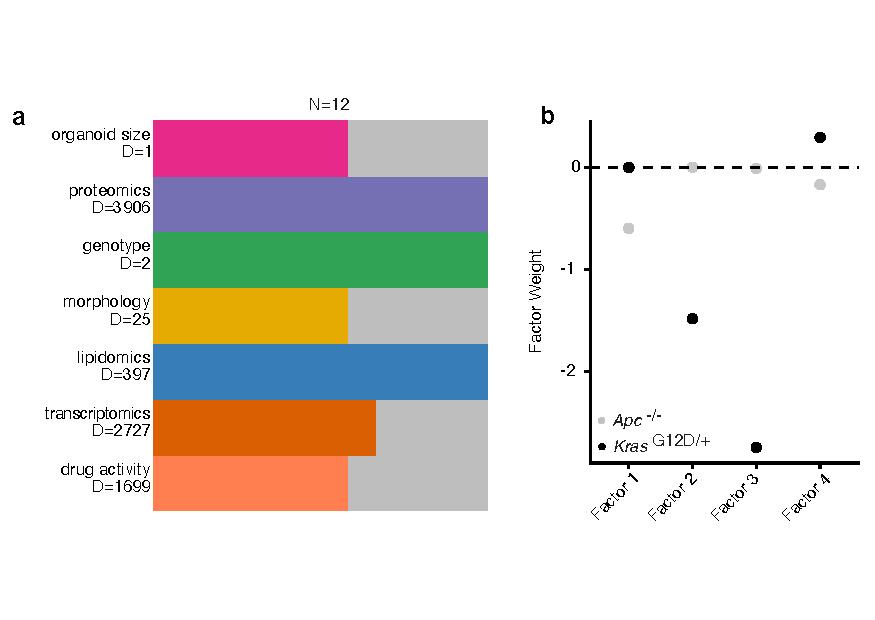
\includegraphics[width=300,
                height=\textheight,
                keepaspectratio]{figures/adenomaprofiling/pdf/fig_1_8.pdf}
\caption{\textbf{Multi-omics factor analysis input data and loadings. a} measurement modalities, dimensionality and number of measurements. A third replicate of measurements were available for proteomics and lipidomics only. \textbf{b} Factor loadings for genotype information.} 
\label{fig_180}
\end{figure}
\bigbreak

\section{A canonical Wnt signaling associated program caused by Apc loss}

To understand the molecular changes associated with factor 1, factor loadings for mRNA expression data were analyzed using Reactome gene-set enrichment analysis (Figure \ref{fig_190} a). Three clusters of biological processes were significantly associated with a negative factor loading, caused by Apc loss-of-function: 1) Mitotic Anaphase related processes, including spindle checkpoints; 2) Mitotic S-phase, including DNA replication and 3) DNA repair mechanisms, including homology directed repair. 

\smallbreak
In line with the enrichment of processes seen in cell proliferation, factor 1 loadings were associated with an enrichment of a previously described intestinal proliferation signature (Figure \ref{fig_190} c) and an LGR5+ instestinal stem cell identity signature (Figure \ref{fig_190} b). These findings are in line with the long-standing evidence that loss of Apc leads to a hyperactivation of canonical Wnt signaling, which in turn leads to increased intestinal cell proliferation and Myc-dependent changes towards a stem-like cell state \cite{Sansom2007-wm, Satoh2017-nd}.


\smallbreak
When focusing on compound activity related factor loadings, a low factor 1 score was significantly linked to increased sensitivity towards small molecules known to target microtubuli and focal adhesion kinase (FAK, Figure \ref{fig_190} d). This morphological sensitivity was presented itself primarily as reduced organoid size and number relative to the DMSO vehicle control (Figure \ref{fig_190} e).

%\begin{figure}[h]
%\centering
%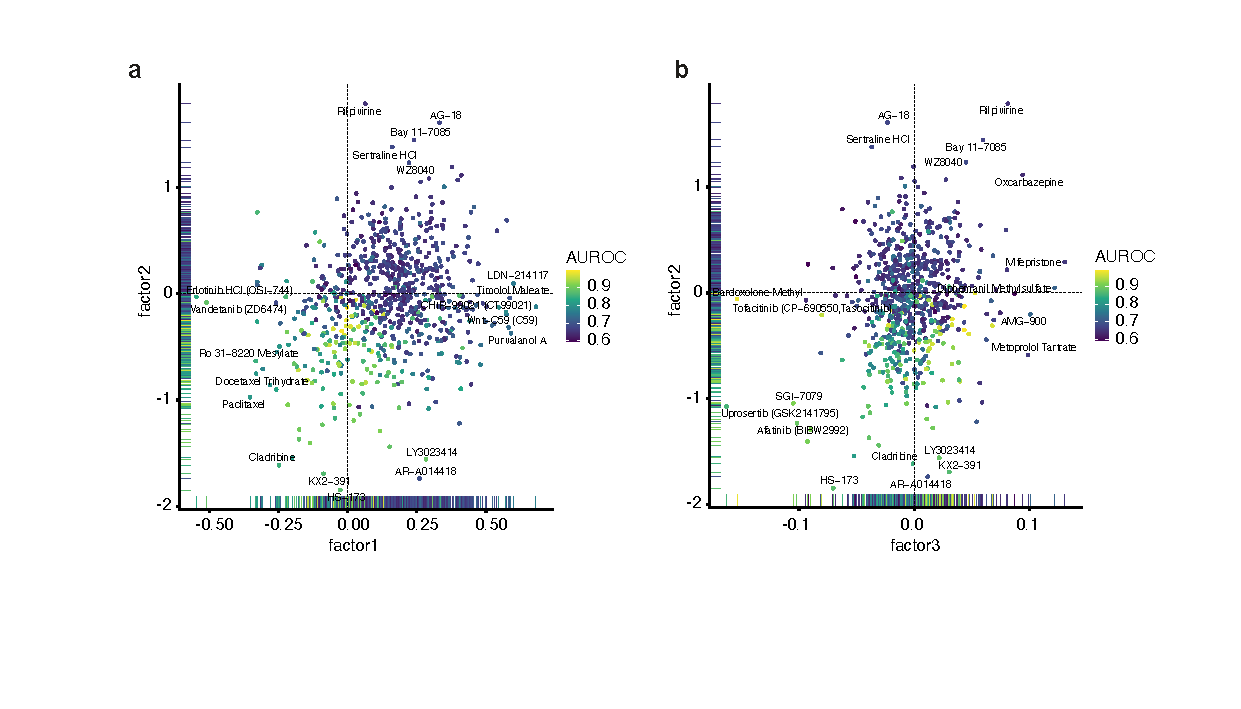
\includegraphics[width=\textwidth,
%                height=\textheight,
%                keepaspectratio]{figures/adenomaprofiling/pdf/fig_1_9.pdf}
%\caption{\textbf{Factor loadings for drug activity. a} Factor 1 and 2 loadings, and \textbf{b} Factor 1 and 3 loadings. Average drug activity score (AUROC) is color coded.}
%\label{fig_180}
%\end{figure}
%\bigbreak

\begin{figure}[h!]
\centering
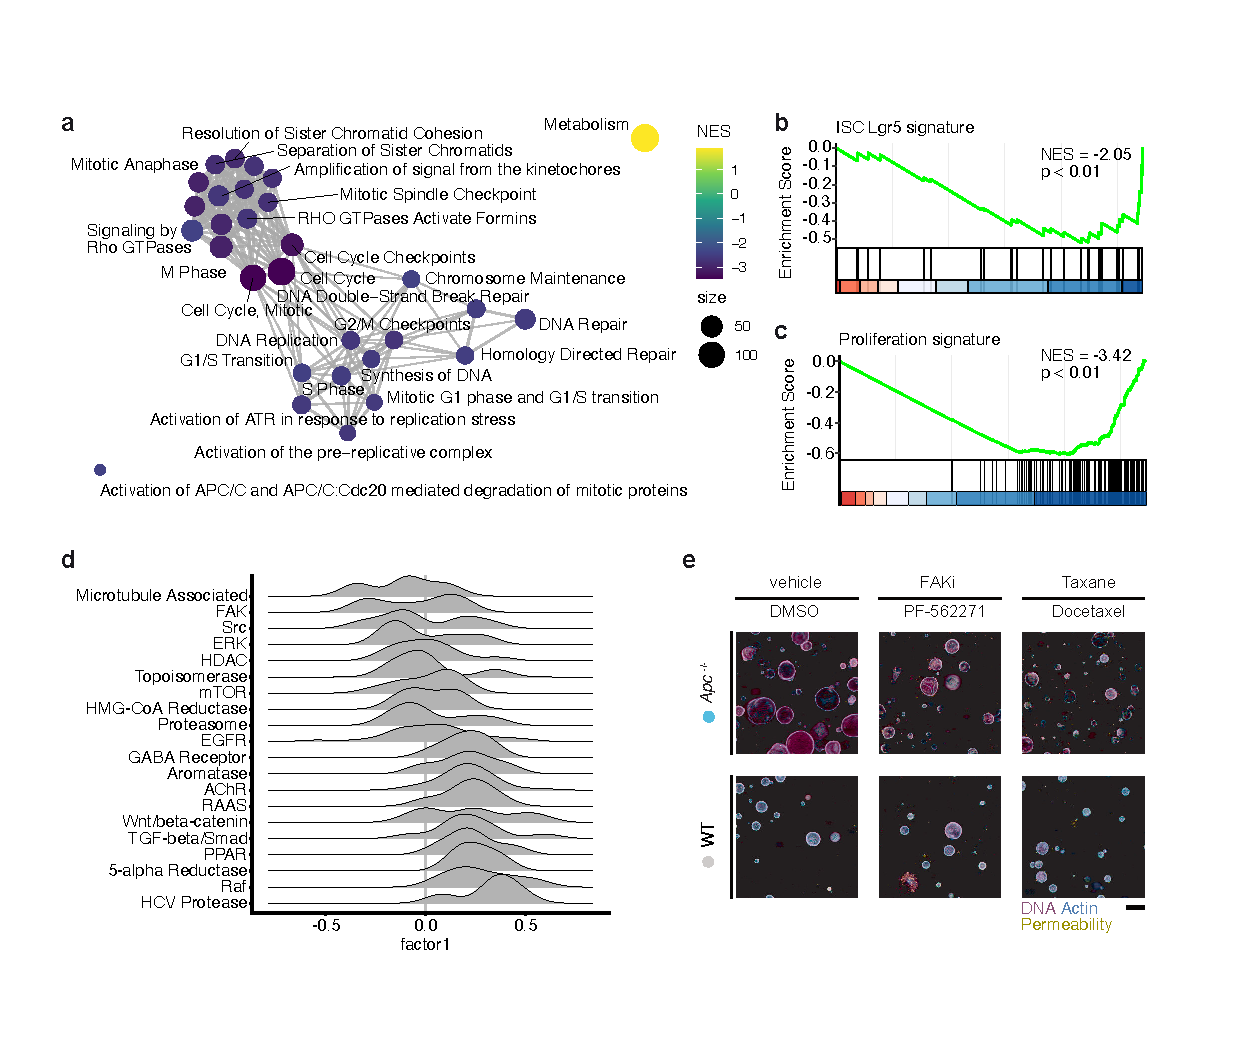
\includegraphics[width=\textwidth,
                height=\textheight,
                keepaspectratio]{figures/adenomaprofiling/pdf/fig_2_1.pdf}
\caption{\textbf{Factor 1, canonical Wnt signaling. a} Gene-set enrichment network of factor 1 gene expression loadings. An edge connects Reactome pathways with more than 20\% overlap. Central enriched processes include mitosis, DNA replication and DNA damage repair. \textbf{b and c} Gene set enrichment results of the "Lgr5 intestinal stem cell" and "proliferation" signature by Merlos-Suarez et al \cite{Merlos-Suarez2011-gd}. over ranked factor 1 gene expression loadings (ranking from high factor 1 loading to low factor 1 loading, NES = normalized enrichment score). \textbf{d} Distributions of drug activity loadings grouped by drug target for factor 1. \textbf{e} Example images of compound treated organoids with WT or Apc-/- genotype. Representaধve images are displayed (magenta = DNA, cyan = actin, yellow = cell permeability, scale-bar: 200μm).}
\label{fig_190}
\end{figure}
\bigbreak

In contrast to microtubuli and FAK inhibitors, the average activity scores of small molecules targeting Wnt signaling was associated with increased factor 1 scores (Figure \ref{fig_190} d). Further exploration of the association between the AUROC activity score and Apc genotype showed that small molecule inhibitors of the canonical Wnt secretion pathway protein Porcupine (Porcn), IWP-L6 and LGK-974, were more active in Apc WT organoids relative to their Apc-/- counterparts \cite{Liu2013-dh} (Figure \ref{fig_199}a). In contrast, this effect was not observable for PRI-724, a small molecule inhibitor targeting the interaction of beta-catenin and CREB-binding-protein \cite{Okazaki2019-gy} (Figure \ref{fig_199}a). These differences in drug activity scores among these small molecule inhibitors are most likely related to their different targets' relative location to Apc in the canonical Wnt signaling cascade. While Porcn-dependent Wnt secretion is generally upstream of the destruction complex, the interaction of beta-catenin and CREB-binding-protein is located downstream of it. As a consequence, inhibition of destruction complex function by loss of Apc is expected to render cells less sensitive to perturbations of the Wnt secretion cascade than perturbations of transcription factor binding properties (Figure \ref{fig_199}b). 

\begin{figure}[h!]
\centering
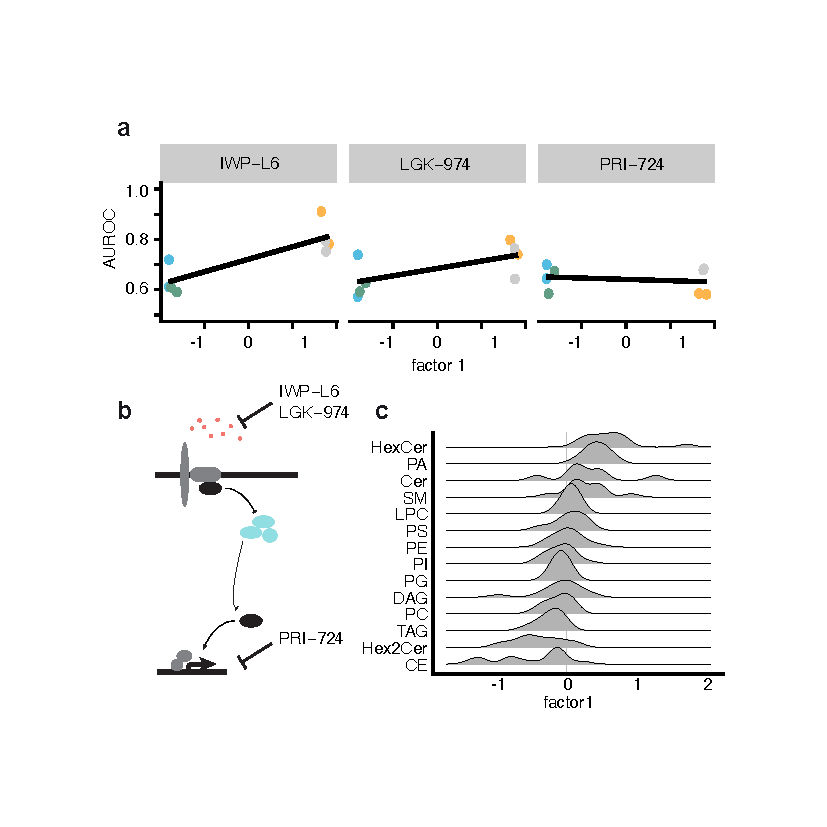
\includegraphics[scale=0.75,keepaspectratio]{figures/adenomaprofiling/pdf/fig_2_2.pdf}
\caption{\textbf{Small molecule Wnt signaling inhibitors. a} AUROC activity score for three small molecule inhibitors of canonical Wnt signaling. \textbf{b} Target proteins for small molecules within the canonical Wnt signaling cascade with their relative position to the destruction complex (highlighted in blue). \textbf{c} Distributions of lipid abundance loadings grouped by lipid species for factor 1 (Abbreviations: HexCer - Hexosylceramide; PA - Phosphatidate; Cer - Ceramide; SM - Sphingomyelin; LPC - Lysophosphatidylcholine; PS - Phosphatidylserine; PE - Phosphatidylethanolamine; PI - Phosphatidylinositol; PG - Phosphatidylglycerol; DAG - Diacylglycerol; PC - Phosphatidylcholine; TAG - Triacylglycerol; Hex2Cer - Dihexosylceramide; CE - Cholersterolester)}
\label{fig_199}
\end{figure}
\bigbreak

Next to factor related differences in morphological compound sensitivity, I analyzed the association of factor 1 weights with measured lipid species. High concentrations of cholesterol esters were associated with a low factor 1 score (seen in Apc-/- organoids), while elevated concentrations of phosphatidic acid species were linked to a high factor 1 score (figure \ref{fig_199}c).

\smallbreak
After linking factor 1 to Apc loss and identifying features caused by this molecular change, I was interested in identifying small molecule treatments that -based on the morphology they induced- shifted organoid state along the factor 1 axis. As described in the previous chapter, small molecules that led to a predicted factor 1 change were identified using ANOVA. To identify treatments that led to a drop in organoid viability, a classifier (LDC) trained on ground-truth lethal treatments within the stem-cell library was applied. Two groups of compounds were identified that induced a shift towards lower factor 1 scores (group A, figure \ref{fig_180}) and higher factor 1 scores (group B, \ref{fig_180}). 

\begin{figure}[h]
\centering
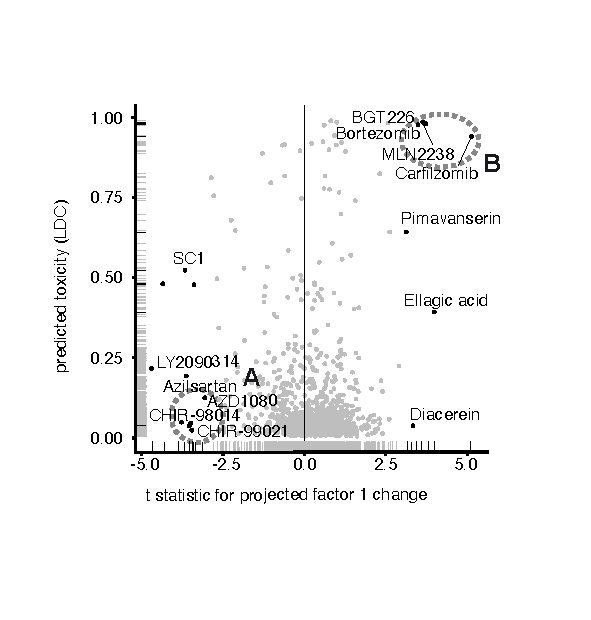
\includegraphics[scale=0.75,
                keepaspectratio]{figures/adenomaprofiling/pdf/fig_2_3.pdf}
\caption{\textbf{Projection of factor 1 scores for treatment-induced phenotypes and viability changes.} Highlighted are compounds leading to a significant change in projected factor scores across all organoid lines (ANOVA). Organoid viability is predicted using a random-forest based classified (LDC) with scores from 0 (no toxicity) to 1 (complete toxicity)}
\label{fig_180}
\end{figure}
\bigbreak

Small molecules within group A induced a morphology associated with Apc loss while maintaining organoid viability. In contrast, members of group B primarily led to a loss of viability and a shift towards a morphological state associated with Apc wildtype organoids. Of note, small molecules within these groups had related target proteins. Compounds within group A (incl. CHIR-98014, CHIR-99021, LY2090314) targeted GSK3 beta - a kinase with central function within the canonical Wnt signaling destruction complex. Inhibition of GSK3 beta leads to hyperactivation of canonical Wnt signaling.
Members of group B primarily targeted the Proteasome (incl. Bortezomib, Carfilzomib, MLN2238).

\begin{figure}[h]
\centering
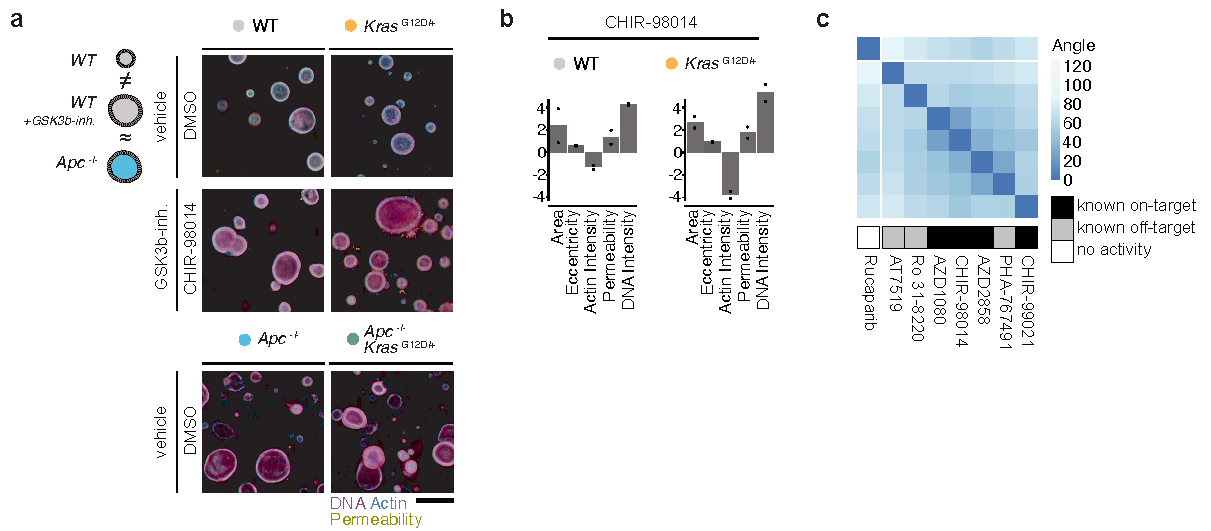
\includegraphics[scale=0.75,
                keepaspectratio]{figures/adenomaprofiling/pdf/fig_2_4.pdf}
\caption{\textbf{GSK3 beta inhibition dependent morphology in colon organoid models. a} Small molecule inhibition of GSK3 beta (CHIR98014) leads to phenocopying of Apc-/- genotype organoid models. \textbf{b} Shift of morphological features relative to scaled population mean for Apc wildtype organoid models treated with CHIR98014. \textbf{c} Excerpt of clustering from figure \ref{fig_150} d, labeled with known binding activity of listed small molecules. Rucaparib is not member of the cluster and shown for comparison.}
\label{fig_185}
\end{figure}
\bigbreak

Further validation of group A showed how treatment with the GSK3 beta inhibitor CHIR-98014 led to treatment-induced phenotypes in WT and KrasG12D+/- organoids that phenocopied the unperturbed morphology of Apc-/- and double mutant organoid models (Figure \ref{fig_185} a). On the feature level, treatment led to an increase in organoid size and DNA intensity (Figure \ref{fig_185} b) in Apc wildtype models. This change in morphology was likely due to an increased proliferation rate of mutant cells, leading to rising organoid size and a higher density of nuclei per analyzed object. Guided by the identification of a strong GSK3 beta inhibition phenotype in Apc wildtype organoids, I analyzed small molecules that clustered with known inhibitors of this kinase based on the angular distance of their drug effect vectors within these models (Figure \ref{fig_185} c) and \ref{fig_150} d). All small molecules clustering with well-described inhibitors of GSK3 beta had previously described off-target binding activity against this kinase within the LINCS KINOMEScan database \cite{Duan2014-ku}.  

\smallbreak
In conclusion of this section, loss of Apc function is the primary source of variation identified across the four analyzed organoid genotypes. Increased cell proliferation rate, canonical Wnt signaling and genomic stress caused by a loss of Apc is observable across profiling modalities and leads to characteristic dependencies (microtubuli, FAK signaling). Small molecules inhibiting the function of the destruction complex member GSK3 beta can phenocopy loss of Apc among colon organoid models.   

\newpage

\section{An oncogene-induced senescence program caused by isolated KrasG12D activation}
% Myc down
While the Apc-/- genotype contributed primarily to factor 1 (Figure \ref{fig_180} b), the KrasG12D allele showed a strong loading for both factor 2 and factor 3. This observation paired with the fact that only organoid models without Apc loss of function were seperated by factor 2 (Figure \ref{fig_170} c), led me to conclude that factor 2 described a KrasG12D dependent change in cell state in the presence of intact Apc function.


\begin{figure}[h!]
\centering
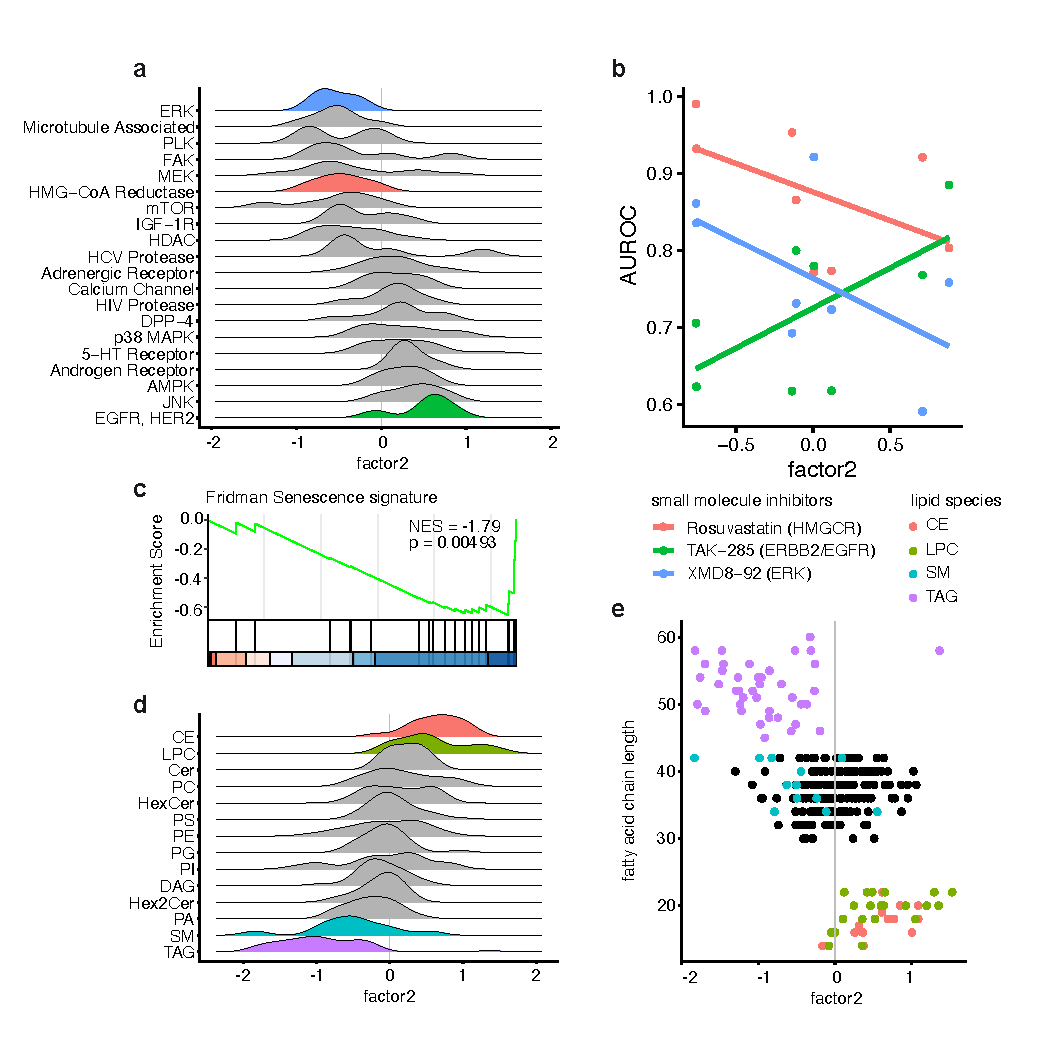
\includegraphics[scale=0.75,
                keepaspectratio]{figures/adenomaprofiling/pdf/fig_3_1.pdf}
\caption{\textbf{Factor 2, KrasG12D induced senescence. a} Distributions of drug activity loadings grouped by drug target for factor 2. \textbf{b} Relationship of representative drugs’ activity with factor 2 score. Shown are compounds from highlighted groups in panel (a). \textbf{c} Gene set enrichment results of a senescence signature by ian et al. over ranked factor 2 gene expression loadings (ranking from high factor 2 loading to low factor 2 loading, NES = normalized enrichment score). \textbf{d} Distributions of lipid abundance loadings grouped by lipid species for factor 2 (Abbreviations: HexCer - Hexosylceramide; PA - Phosphatidate; Cer - Ceramide; SM - Sphingomyelin; LPC - Lysophosphatidylcholine; PS - Phosphatidylserine; PE - Phosphatidylethanolamine; PI - Phosphatidylinositol; PG - Phosphatidylglycerol; DAG - Diacylglycerol; PC - Phosphatidylcholine; TAG - Triacylglycerol; Hex2Cer - Dihexosylceramide; CE - Cholersterolester). \textbf{e} Relationship of acyl chain length with factor 2 loading. Shown are lipids from highlighted species in panel (d)}
\label{fig_200}
\end{figure}
% add Fridmann citationh

\bigbreak
To understand the molecular mechanisms represented by factor 2, I again analyzed features with large absolute loadings for this factor. Plotting of factor loadings for drug activty by small molecule target, showed that ERK and MEK inhibitors were more active in factor 2 low models (KrasG12D+/-) while EGFR/HER2 inhibitors were more active in factor 2 high organoids (WT, figure \ref{fig_200} a and b). This juxtaposition in small molecule activity against RAS-MAPK pathway members was reminiscent of the previous observations made around canonical Wnt signaling inhibitors (Figure \ref{fig_199}). With oncogenic Kras localized between the receptor-layer (including Egfr and Her2) and downstream kinases (for example Erk), hyperactive Kras signaling likely leads to a cell state with relative resistance to EGFR inhibitors and increased dependency on Erk signaling. The previously observed transcriptional process of Egfr-downregulation as a response to KrasG12D+/- is in line with these observations (Figure \ref{fig_162}b).

\smallbreak

In addition, HMG-CoA reductase inhibitors (incl. Rosuvastatin) showed an increased activity in KrasG12D+/- organoids (Figure \ref{fig_200} a and b). This vulnerability towards cholesterol biosynthesis inhibitors in cells with oncogenic Kras signaling has previously been discussed \cite{Yu2018-he}. 

\smallbreak
Oncogene induced senescence is a cell state marked by an arrest of the cell cycle and expression of pro-inflammatory mediators as a response to an oncogenic perturbation. An activated KrasG12D+/- genotype leads to oncogene induced senescence of colon epithelial cells in vivo \cite{Bennecke2010-zf}. 

\smallbreak
Prompted by previous reports on the effect of oncogenic Kras, I identified an enrichment of a senescence related gene expression signature by Fridman et al. within the loadings of factor 2 
\cite{Fridman2008-ky} (Figure \ref{fig_200} c). Transcripts linked to cell senescence, including Igfbp3 (factor 2 loading ca. -0.999) and Hmga2 (factor 2 loading ca. -1.050) ranked among the strongest contributors to the factor. 

\smallbreak
Further exploration of loadings for factor 2 revealed systematic shifts in the composition of the lipidome. Activation of oncogenic Kras led to an accumulation of sphingomyelin (SM) and triacylglycerol (TAG) species in colon cells. In contrast, I observed a relative depletion of cholesterol esters (CE) and lysophosphatidylcholine (LPC) (Figure \ref{fig_200} d). Next to shifts in the lipid comoposition, I also observed a correlation of fatty acid residue chain length and factor 2 loadings, where a low factor 2 score was correlated with higher residue chain length (Figure \ref{fig_200} e) and a higher degree of lipid desaturation (data not shown). Both of these association was primarily driven by differences in the abundance of lipid species, however. 

\smallbreak
To summarize, factor 2 explains differences between wildtype and KrasG12D+/- organoid models and captures the activation of RAS-MAPK signaling and subsequent oncogene induced senescence. KrasG12D+/- transformed colon cells showed a hyperactivation of RAS-MAPK signaling with characteristic changes in small molecule dependencies (ERK and EGFR inhibitors, respectively). Of note, KrasG12D+/- induced senescence coincided with the accumulation of triacylglycerol (TAG) and sphingomyelin (SM) species within colon organoids. Lipid accumulation in senescent cells has been observed in multiple senescent cells, including human fibroblasts (TAG accumulation) \cite{Lizardo2017-uy} and, more specifically, has recently been described in non-mammalian model systems as a consequence of Kras mediated oncogene induced senescence \cite{Yao2018-ut}. 

%\begin{figure}[h]
%\centering
%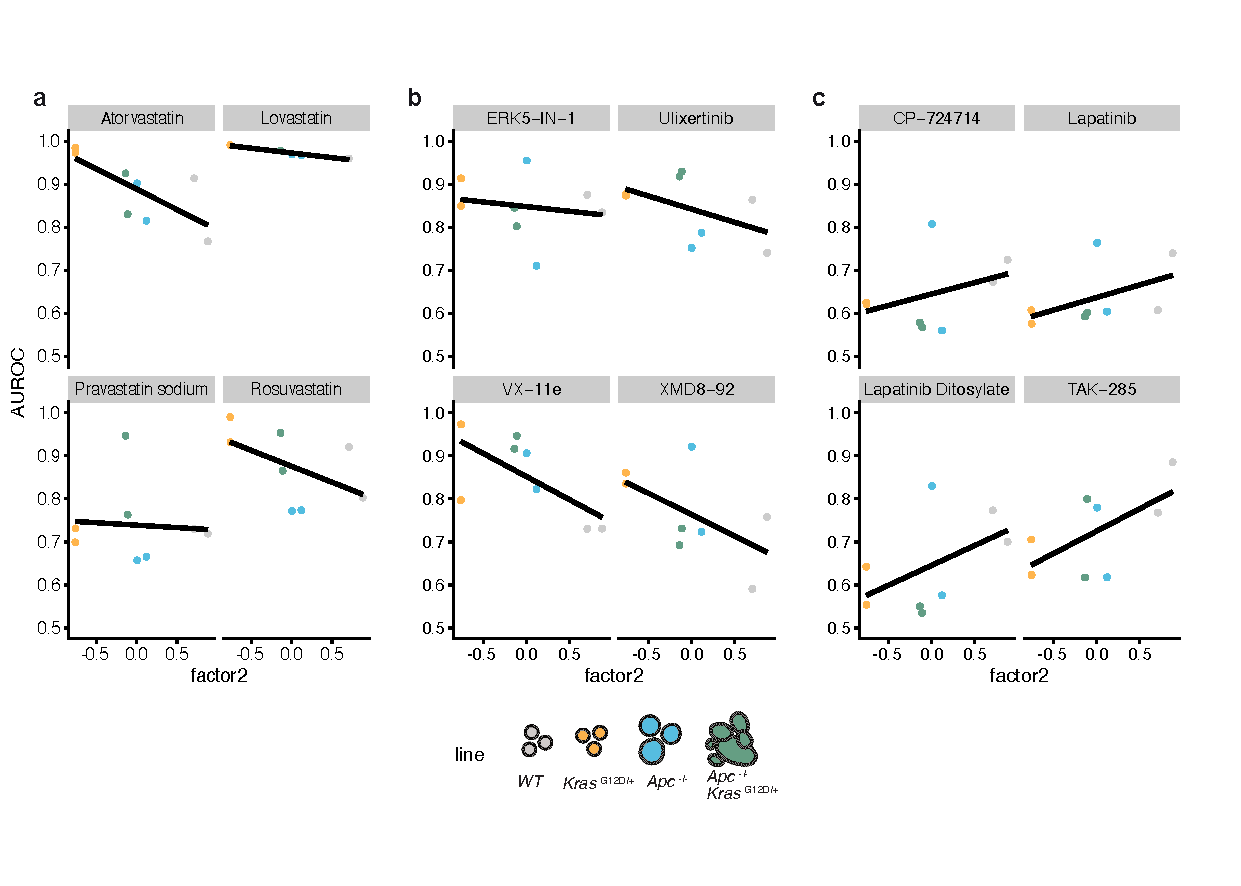
\includegraphics[width=\textwidth,
%                height=\textheight,
%                keepaspectratio]{figures/adenomaprofiling/pdf/fig_3_2.pdf}
%\caption{}
%\label{fig_180}
%\end{figure}
%\bigbreak

%\begin{figure}[h]
%\centering
%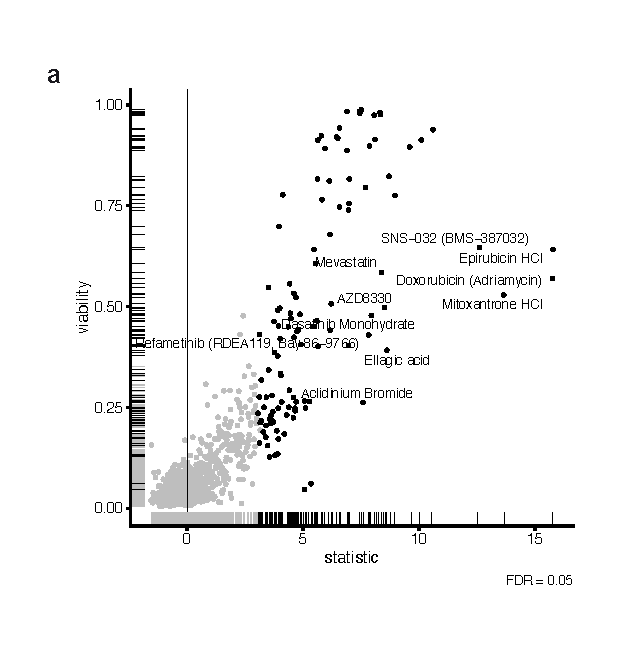
\includegraphics[width=\textwidth,
%                height=\textheight,
%                keepaspectratio]{figures/adenomaprofiling/pdf/fig_3_3.pdf}
%\caption{}
%\label{fig_180}
%\end{figure}
%\bigbreak

\newpage
\section{oncogenic Kras leads to increased mTOR signaling in the context of Apc loss of function}

While factor 2 captured the effect of oncogenic Kras in an Apc wildtype state, factor 3 scores separated organoid models by Kras genotype in the context of an Apc loss of function (Figure \ref{fig_170} c). On average, factor 3 only accounted for ca. 10\% of variance across modalities within the MOFA model, supporting the overall similarity of Apc-/- and Apc-/- KrasG12D+/- organoids previously observed on the transcriptome, proteome, lipidome and phenotype level (Figure \ref{fig_161}a-d and \ref{fig_140} b).

\begin{figure}[h]
\centering
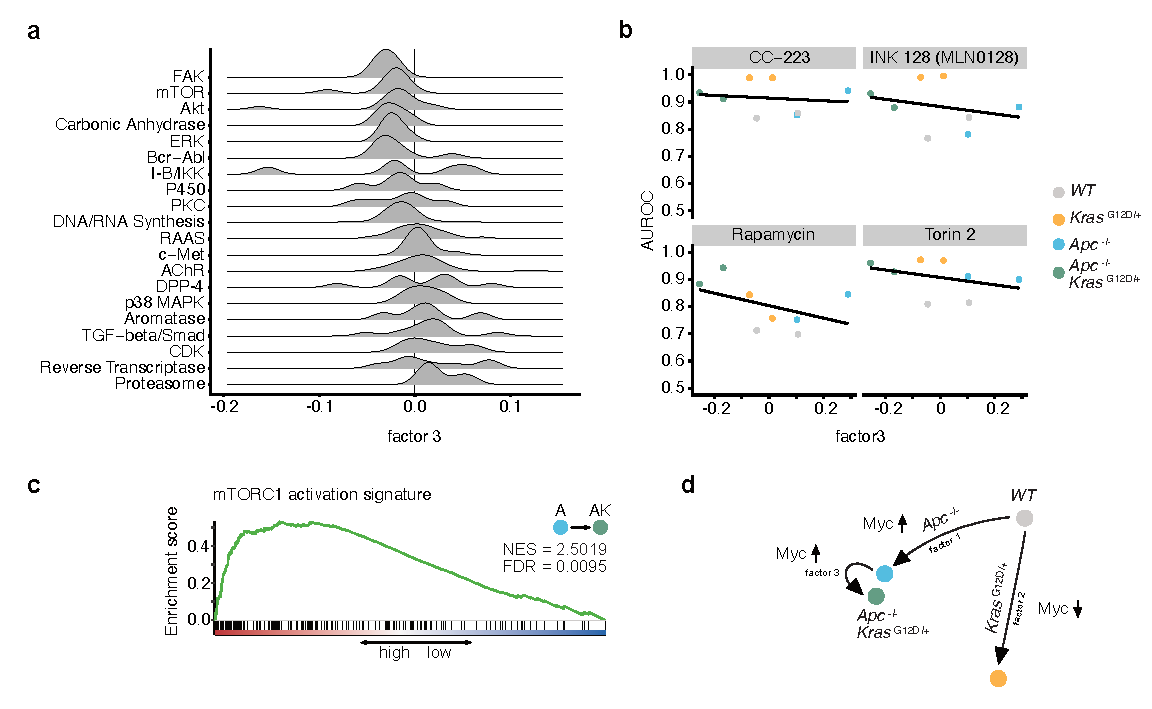
\includegraphics[scale=0.75,
                keepaspectratio]{figures/adenomaprofiling/pdf/fig_4_1.pdf}
\caption{\textbf{Factor 3, KrasG12D effects in the context of Apc loss of function. a} Distributions of drug activity loadings grouped by drug target for factor 3. \textbf{b} Relationship of representative mTOR inhibitor activity with factor 3 score. \textbf{c} Gene set enrichment results of a Reactome mTORC1 activation signature over ranked factor 3 gene expression loadings (ranking from high factor 3 loading to low factor 3 loading, NES = normalized enrichment score). \textbf{d} Visual summary of Myc gene set enrichment results for organoid state transitions. Myc signatures were significantly enriched in Apc-/- models and depleted in models with isolated KrasG12D+/- mutation.}
\label{fig_300}
\end{figure}
\bigbreak

Exploration of factor 3 loadings identified mTOR and FAK inhibitors to systematically contribute to a negative factor score. Double-mutant organoid models (Apc-/- KrasG12D+/-) were more sensitive to these small molecule inhibitors than their single-mutant Apc-/- counterparts (Figure \ref{fig_300} a). This difference in drug activity was observerable for both ATP-competitive (e.g. INK-128, Sapanisertib) and non-ATP-competitive (e.g. Rapamycin) inhibitors (Figure \ref{fig_300} b). In line with the increased sensitvity to mTOR inhibitors, differential gene expression analysis comparing single (Apc -/-, abbreviated A) and double mutant (Apc-/- KrasG12D+/-, abbreviated AK) organoids identified a significant increase in mTORC1 activation according to a Reactome signature (Figure \ref{fig_300} c, FDR=0.0095, NES=2.5019). 

\smallbreak
Further exploration of factor 3 loadings in gene expression space showed an enrichment of multiple Myc target gene signatures \cite{Yu2005-em, Zeller2003-ok}. Transcription signatures associated with increased Myc activity are enriched in double-mutant organoid models (Apc-/- KrasG12D+/-) when compared to single-mutant counterparts (Figure \ref{fig_300} d). In fact, further analysis of factor 1 and factor 2 gene expression loadings identified significant changes in Myc activity signatures for both factors as well. Simplified, loss of function of Apc led to an increased activity of Myc (factor 1) while the isolated presence of oncogenic KrasG12D+/- led to a reduced activity of Myc. These observations are consistent with previous studies describing a central role of increased Myc activity in Wnt-signaling dependent adenoma formation \cite{Satoh2017-nd} and decreased Myc activity in oncogene induced senescence \cite{Yao2018-ut}.

\smallbreak
In summary, factor 3 is representing the interaction of Apc loss of function and oncogenic KrasG12D+/-. In the mouse colon organoid model, the introduction of oncogenic KrasG12D+/- within an Apc-/- background leads to an increased mTORC1 signaling related gene expression signature and increased sensitivity to small molecule mTOR inhibitors. Myc activity related gene expression is increased in all factors related to malignant transformation, except the introduction of isolated oncogenic KrasG12D+/- in where Myc activity is reduced in line with the oncogene induced senescence model. 

\newpage
\section{Ellagic acid is a candidate small molecule revertant therapeutic of organoid adenoma states}

Similar to the analysis in the previous chapter, I searched for treatments which induced organoid phenotypes that suggested a change of organoid state within the learned factor-space. Treatments that were predicted to move organoids towards a wildtype state along factor 1 and 2 were of particular medical relevance. Analogous to the concept of revertant genetic mutations, I referred to small molecules with a predicted ability to move transformed organoids towards a wildtype state as potential revertant therapeutics.

\begin{figure}[h]
\centering
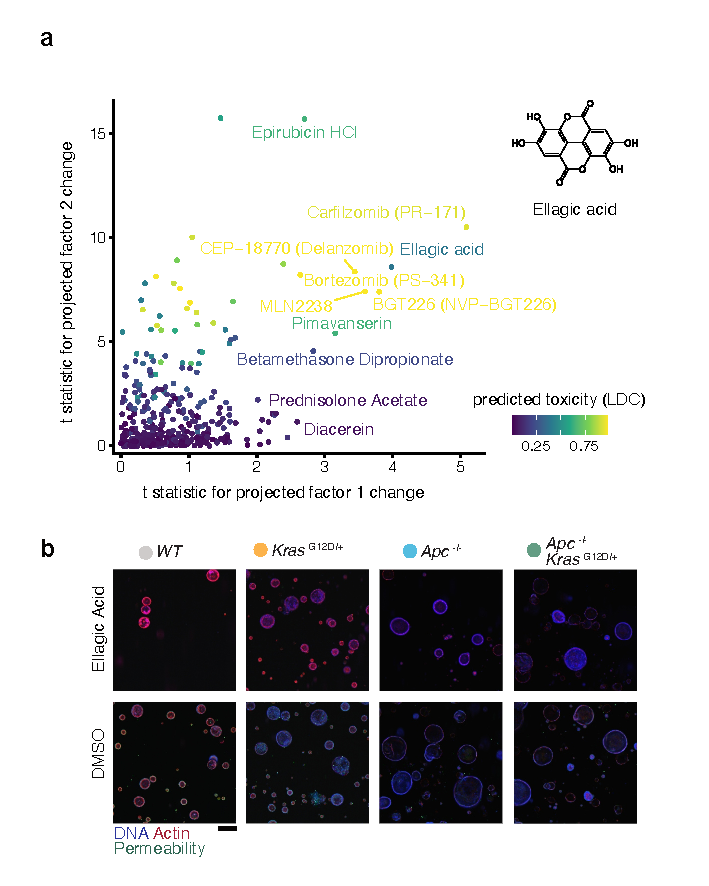
\includegraphics[scale=0.75,
                keepaspectratio]{figures/adenomaprofiling/pdf/fig_5_1.pdf}
\caption{\textbf{Projected changes in factor 1 and 2 scores after small molecule treatment a} Shows are treatments leading to change in projected factor scores across all organoid lines (ANOVA). Color coding represents predictions based on LDC viability classifier. The structural formula of Ellagic Acid is depicted in the top right. \textbf{b} Organoid treatment with Ellagic acid. Depicted are representative example images for each line (blue = DNA, red = actin, green = cell permeability, scale bar=200µm).}
\label{fig_310}
\end{figure}
\bigbreak

The majority of compounds that led to a predicted shift towards a wildtype organoid state along both axes were also associated with a high predicted toxicity (Figure \ref{fig_310} a, color coding are predictions based on LDC viability classifier). Ellagic acid, however, a natural compound that was predicted to function as a revertant, showed a moderate predicted toxicity (Figure \ref{fig_310} a, top right). Inspection of organoid models treated with Ellagic acid showed reduced number and size of organoids compared to the vehicle control, while organoid viability was generally maintained (Figure \ref{fig_310} b). 

\bigbreak
In this chapter I hypothesized that image-based profiling of engineered organoid models can help identify small molecule candidates that move organoids within a well-defined multi-omics representation space. Analysis of four genetically defined organoid models resulted in three interpretable joint factors within the MOFA analysis. Exploration of factors revealed that Kras G12D dependent oncogene induced senescence in colon organoids is accompanied with characteristic changes to the lipidome, which are not observable in Apc mutant organoid models. Known small molecule inhibitors of GSK3 beta were predicted to move organoid in factor space along factor 1, a canonical Wnt-signaling associated program. Ellagic acid, a natural compound, was predicted to move organoid phenotypes towards an unperturbed morphology, prompting further validation.
\end{flushleft}
\begin{flushleft}

\chapter{Discussion}

\section{Disclosure}
Parts of the discussion, in particular the section \textit{"Two multi-omics factors defining patient-derived colorectal cancer organoid phenotype"}, have been adapted from a joint first-author publication, \textit{The drug-induced phenotypic landscape of colorectal cancer organoids} \parencite{betgeDruginducedPhenotypicLandscape2022}. The adapted text was originally written by myself.


\section{Image-based profiling of organoids}

\subsection{Using organoids as high validity \textit{in-vitro} models for image-based profiling}

Organoids are representative \textit{in-vitro} models for diverse human tissues and can be used for image-based profiling. While the prospective use of cancer organoids as a diagnostic is currently limited by high sample dropout and long turnaround time, a high overall predictive validity for multiple therapeutic regimens has been reported \parencite{ooftProspectiveExperimentalTreatment2021}. The use of organoid models in early-stage drug discovery, however, is not limited by the same constraints existing in a diagnostic context. For therapeutic discovery, previous studies have successfully used organoids to perform medium-scale small molecule treatment assays. The most commonly used method is screening with an ATP-based cell viability readouts \parencite{vandeweteringProspectiveDerivationLiving2015}. Additionally, imaging studies with organoids have been used to characterize developmental processes such as the self-organization of intestinal cells \parencite{lukoninPhenotypicLandscapeIntestinal2020, boehnkeAssayEstablishmentValidation2016a} or the morphological response to individual drugs \parencite{Badder2020-au, serraSelforganizationSymmetryBreaking2019}. While image-based profiling of \textit{in-vitro} models has become an important method in functional genomics and therapeutic discovery \parencite{carpenterImagebasedChemicalScreening2007}, performing such high-throughput experiments in organoid models has been a technological challenge given the 3D multicellular growth pattern of organoids as well as their required culture conditions. In this thesis, sparse 3D imaging as well as adjustment to the seeding and staining protocol enabled small molecule image-based profiling of patient-derived and genetically engineered colorectal cancer organoid models. 
\bigbreak


\subsection{Towards multi-view profiling}
A challenge in image-based profiling is the low interpretability of the morphological representation that is generated during the image analysis step. Classic quantitative features of cellular morphology are rarely descriptive, and even when dimensionality reduction methods or self-supervised learning techniques are used, the learned representations are rarely directly interpretable within the context of cellular mechanisms. To increase the interpretability of observations in a given image-based profiling experiment, supporting multi-view data, for example transcriptomics, proteomics or metabolomics data can be collected to "annotate" images. A simple and idealized approach to perform such annotation would be to collect the complete multi-view information for all tested treatment conditions (i.e., imaging, transcript abundance, protein abundance, lipid abundance). However, both from a physical (some measurement methods destroy the sample) and cost perspective, this approach is inaccessible. 
\smallbreak

In this thesis, an alternative model-based approach was chosen to increase the interpretability of morphology information: First, a well-annotated multi-view representation of untreated organoids was learned by modeling morphological features as well as molecular features (i.e., transcript expression). In a second step, single-view treatment-induced morphologies were projected into the learned representation. The resulting factor scores were used to identify treatments with an interpretable effect. Examples of such identified effects include (1) the increase in organoid size and IGF1R-signaling as a response to mTOR inhibition (factor 1, patient-derived organoids); (2) the spherical reorganization and increase in LGR5 transcript expression as a response to MEK inhibition (factor 2, patient-derived organoids); as well as (3) the increase in organoid size, DNA staining intensity and canonical Wnt signaling as a response to GSK3-beta inhibition (factor 1, mouse organoids). While this approach has utility in guiding the interpretation of otherwise challenging-to-interpret morphology information, a series of important limitations exist that are outlined below.
\smallbreak

A central limitation of the described multi-view representation learning approach are \textbf{out of distribution observations} during the projection of treated organoids. Observations during factor-learning were drawn from an untreated distribution of organoid states, while projected observations were drawn from a distinct distribution of treated organoids. As a result, an observed treatment within the query set that is far outside the distribution learned from the support set is likely to be misinterpreted. For example, if observation from \textit{Apc} mutant organoid lines had not been included in the support set that the multi-view representation was learned from, the effect of GSK3-beta inhibitors on \textit{Apc} wild type organoids would not have been interpretable. These treatment-induced morphologies would have been grouped with the set of non-specific but active treatments, such as Proteasome inhibitors. In this thesis, potential out-of-distribution treatments were identified through a high AUROC score and non-specific treatment effects along multiple factors. In the future, more principled methods to detect out-of-distribution samples, such as obtaining the likelihood or reconstruction error, could be used. Given the limitation of out of distribution observations, it is important to include conditions in the support set that are well annotated \textbf{and} representative of the effects that are supposed to be explored, as the representation learned from this data will be used to interpret all remaining observations within the query set. Put differently, a support set needs to be constructed with the biological question in mind because all other observations will be interpreted using a model that was learned from it.
\smallbreak

A second limitation associated with the used approach is a \textbf{lack of causality} in the interpretation of treatment effects on factors. For example, CDK inhibitors led to a decrease in factor 1 scores among patient-derived colorectal cancer organoids, with a markedly smaller organoid size in treated organoids. This decrease in factor 1 scores does, however, not inform about the causal structure of the mechanism that is leading to a shift in factor 1. For example, while all the following causal diagrams are as likely in the light of the factor score shift, they are distinct in terms of their biological plausibility: It is unlikely that CDK is a regulator of IGF1R signaling (CDK → IGF1R → organoid size), while it is more likely that CDK is a mediating variable of IGF1R signaling (IGF1R → CDK → organoid size) or an independent effector (IGF1R → organoid size, CDK → organoid size). In summary, treatment effects on factors aid in the generation of hypotheses but need to be used as a starting point for further validating experiments.
\smallbreak

A third limitation of this approach is \textbf{data drift}. This limitation is most likely relevant in the context of larger profiling campaigns: Over the course of multiple experimental batches, the distribution of morphology states that is observed for both untreated and treated organoids is shifting. A model that has been trained at day 1 on a distribution of untreated organoid phenotypes and is used to interpret phenotypes on day 30 of treated organoids might show unexpected behavior because of a shift of experimental conditions, i.e., the staining protocol. The conditions in the experiments performed during this thesis were not fully representative of such scenarios, as untreated and treated organoid morphologies were collected in parallel and all morphological data were pre-processed together (i.e., features scaling, PCA transformation). As a result, the ability of multi-view group factor analysis to project "unseen" treatment induced morphologies into interpretable factors was assessed under idealized conditions with considerable data leakage, which needs to be accounted for if using such an approach in larger discovery or diagnostic projects.
\par
\bigbreak

Despite these limitations, the combination of multi-view representation learning and image-based profiling of organoids introduced in this thesis has the potential to be built upon and improved. A set of possible directions exist, such as (1) further increasing the predictive validity of in-vitro models by imaging organoid models within co-culture systems \parencite{cattaneoTumorOrganoidCell2020}; (2) further increasing the robustness of multi-view profiling by introducing selective RNA-Sequencing of formalin fixed cells after a microscopy run is completed; and (3) improving the image analysis and modeling process by using self-supervised learning methods instead of classical morphological features \parencite{perakisContrastiveLearningSingleCell2021}.

\clearpage
\section{Multi-view profiling of patient-derived colorectal cancer organoids identifies factors of cancer organoid architecture}

A set of 11 patient-derived colorectal cancer organoids were profiled to understand the underlying factors determining organoid morphology, as well as characteristic differences in small molecule sensitivity.

\subsection{Two multi-omics factors defining patient-derived colorectal cancer organoid phenotype}

The first identified axis of phenotype variation was an IGF1R signaling program associated with increased organoid size, EGFR inhibitor resistance, which can be induced by mTOR inhibition. Insulin-like growth factors are central and conserved regulators promoting cell size, organ size and organism growth \parencite{pucheHumanConditionsInsulinlike2012, sunMechanismCellSize2006}. The IGF1 receptor (IGF1R) signaling cascade is activated in around 20\% of colorectal cancer patients and leads to downstream mitotic stimuli via ERK-MAPK signaling and mTOR \parencite{zhongOverproductionIGF2Drives2017}. In patient-derived cancer organoids, we observed that average organoid size was positively correlated with elevated IGF1R signaling activity, as determined by transcript expression.
\smallbreak

Increased IGF1R signaling activity also presented with a characteristic pharmacological sensitivity profile. In accordance with previous observations\parencite{isellaSelectiveAnalysisCancercell2017}, colorectal cancer organoids in a high IGF1R signaling state were less responsive to EGFR inhibitors and more responsive to IGF1R and MEK blockade, demonstrating the central role of IGF1R mediated mitogen activated protein kinase (IGFR1-MAPK) signaling. In fact, reciprocal resistance between IGF1R and EGFR signaling inhibitors has been described in multiple cancer types \parencite{huaInsulinlikeGrowthFactor2020a}. Moreover, organoids could be moved into a state of increased IGF1R-MAPK signaling by inhibition of mTOR, a downstream mediator of IGF1R activity. In line with this observation, a reactive induction of IGF1R signaling has been previously described as a resistance mechanism to small molecule mTOR inhibitors in cancer \parencite{sharmaChromatinmediatedReversibleDrugtolerant2010, yoonFocalAdhesionIGF1RDependent2017a}. 
\smallbreak

Its role in controlling cell size and the high number of interactions with other signaling mechanisms, such as EGFR and mTOR, have made IGF1R signaling an attractive target for therapeutic discovery. So far, however, neither mono- nor combination therapies containing IGF1R receptor inhibitors have shown clinical utility \parencite{beckwithMinireviewWereIGF2015, jentzschCostsCausesOncology2023}. A speculative explanation for this failure in clinical trials might be related to its signaling network centrality. While the IGF1R receptor and its downstream effectors are central mediators of growth-stimulating processes, they do not themselves constitute a necessary condition for tumor growth \parencite{beckwithMinireviewWereIGF2015}, which is, in contrast, often the case for genetic events involved in disease development, such as \textit{APC} loss-of-function \parencite{dowApcRestorationPromotes2015a} or \textit{KRAS} gain-of-function. 
\smallbreak

While the potential of IGF1R as a target for therapeutic discovery is low in light of past evidence, direct implications for the method of organoid culture - in particular the role of supplementing IGF-1 to increase organoid growth \textit{in-vitro} - might be drawn from the results of this study. Next to the observation that organoids with strong IGF1R signaling were of greater average size, the emerging role of IGF1R signaling in organoid culture was recently emphasized by the observation that addition of the IGF-1 ligand, relative to EGF, increased culture efficiency of organoids from healthy human intestinal tissue \parencite{fujiiHumanIntestinalOrganoids2018a}. Given the association of IGF1R signaling with organoid size within this thesis as well as the observation from organoid isolation studies \parencite{fujiiHumanIntestinalOrganoids2018a}, I hypothesize that addition of IGF-1 ligand to colorectal cancer organoid culture media could (1) further increase culture establishment efficiency and (2) reduce additional genetic bottleneck effects that might bias isolated organoid cultures towards increased IGF1R signaling.
\smallbreak

The second axis of phenotype variation was an LGR5+ program associated with cystic organoid architecture and Wnt signaling inhibitor sensitivity, which can be induced by inhibition of MEK. Organoid models with a high factor score showed a monolayer organization with a characteristic actin cytoskeleton and an enrichment of an LGR5 intestinal stem cell signature along the factor weights. These LGR5+ organoids were more sensitive to Wnt inhibitor (Pri-724) treatment and showed a relative resistance to Erk and Mek small molecule inhibitors. Surprisingly, not only were organoids in this stem-like state more morphologically resistant to Mek inhibition, treatment with Mek inhibitors shifted organoids towards this LGR5+ state. Put differently, a subset of organoids which are LGR5+ are insensitive to MEK inhibition and Mek inhibition drives (surviving) organoids towards this LGR5+ state.
\smallbreak

The ability of ERK-MAPK inhibition (here EGFR and MEK) to move intestinal organoids into a quiescent LGR5+ state was described by \parencite{basakInducedQuiescenceLgr52017} and led to a "clutch and gas pedal" model of Wnt and ERK-MAPK signaling in which Wnt signaling is necessary and sufficient to maintain the LGR5+ stemlike state, while ERK-MAPK signaling is a primary signal to cause (stem cell) proliferation \parencite{basakInducedQuiescenceLgr52017}. Additional work by \parencite{zhanMEKInhibitorsActivate2019a} recently extended this model by demonstrating that inhibition of MEK in colorectal cancer cell lines and organoid models leads to an increase in canonical Wnt signaling through inhibition of EGR1-dependent transcription of AXIN1, a necessary member of the destruction complex. According to this extended model, Wnt signaling is necessary and sufficient to maintain the LGR5+ cell state, and ERK-MAPK signaling is not only the primary proliferative signal, but its inhibition can even further shift the cellular state towards the LGR5+ identity. 

\clearpage
\subsection{Are patient-derived organoids representative of known molecular colorectal cancer states?}

The multi-view factors that were identified in patient-derived organoids during this thesis capture differences in IGF1R-, EGFR-, and canonical Wnt signaling (high Factors 1, low Factor 1, and high Factor 2, respectively). A natural question to ask is whether the identified molecular axes of variation are aligned with previously identified molecular axes or variation (and the states they define) of colorectal cancer tissue samples. Molecular states, also referred to as subtypes, of colorectal cancer have been proposed by a series of consortia and are often centered around a single data modality. Most common subtype classifications are based on bulk transcript expression data \parencite{guinneyConsensusMolecularSubtypes2015} while other classifications, for example based on single-cell transcript expression \parencite{joanitoSinglecellBulkTranscriptome2022}, have been developed. The Consensus Molecular Subtypes (CMS) classification \parencite{guinneyConsensusMolecularSubtypes2015} is among the most widely used subtype classifications and was developed by a consortium of researchers that had previously published multiple independent classifications. The CMS classification groups colorectal cancer tissue samples that have undergone bulk transcript expression measurements into four subtypes that are summarized briefly below:

\begin{itemize} 
    \item CMS 1: hypermutated, frequently BRAF-mutated, MSI and CIMP samples with corresponding signs of inflammation
    \item CMS 2: high Wnt signaling activity, chromosomal instability (CIN) common
    \item CMS 3: \textit{KRAS}-mutated MSS samples, signs of strong metabolic deregulation
    \item CMS 4: stromal infiltration and high TGF-beta activation, worse overall survival
\end{itemize}

Since its publication \parencite{guinneyConsensusMolecularSubtypes2015}, however, the classification has not found use in clinical care. Two prospective studies in which the CMS classifier was applied and the treatment choices of Cetuximab vs. Bevacizumab (both in combination with FOLFIRI/FOLFOX) were evaluated, came to -at first sight- conflicting conclusions \parencite{stintzingConsensusMolecularSubgroups2019, lenzImpactConsensusMolecular2019, aderkaExplainingUnexplainableDiscrepancies2019, sveenPredictiveModelingColorectal2019}. While one group concluded that the CMS classification had "no direct impact on clinical decision-making" \parencite{stintzingConsensusMolecularSubgroups2019,} the other group concluded that their "findings highlight the possible clinical utility of CMS" \parencite{lenzImpactConsensusMolecular2019}. While a range of specific explanations for this particular discordance have been proposed (i.e., cohort differences in UICC stage, pretreatment history, and chosen chemotherapy backbone), a set of general observations that highlight current limitations of clinical transcriptome measurement and classification that go beyond the use of the CMS classifier itself might be more instructive for this discussion: 

\begin{itemize} 
    \item Clinical transcriptome measurements and classification of multiple biopsies from the same patient can give discordant results, for example when comparing primary tumor and metastasis \parencite{eideMetastaticHeterogeneityConsensus2021}  
    \item Clinical transcriptome measurements and classification are still not a standardized procedure, thereby reducing their reliability \parencite{sveenPredictiveModelingColorectal2019}. Different transcript expression measurement methods and software libraries are used —even between clinical trials that aim to use the same classification \parencite{stintzingConsensusMolecularSubgroups2019, lenzImpactConsensusMolecular2019}.
    \item Clinical transcriptome measurements capture and classify the whole tumor sample, including the tumor microenvironment surrounding the malignant cells. In such contexts, it is generally challenging to draw conclusions for the malignant cells in isolation.
\end{itemize}

Especially because the CMS classification was established on whole tissue samples, and not isolated malignant cells, care should be taken when comparing subtype classifications between in-vitro models and clinical samples. Within the collection of patient-derived organoids profiled within this study, the majority of organoids were classified as CMS2 (11/13). Of note, no CMS1 or CMS4 organoid lines were established. This distribution of assigned subtypes was in line with reports from other colorectal cancer organoid studies \parencite{vandeweteringProspectiveDerivationLiving2015, schutteMolecularDissectionColorectal2017} and showed an under-representation of CMS1 and CMS4. Motivated to identify a possible alignment with published classification systems, I noticed a partial alignment of modeled states with the colorectal cancer intrinsic subtype (CRIS) model \parencite{isellaSelectiveAnalysisCancercell2017a}. The CRIS model was identified based on transcriptomic data from patient-derived xenografts (PDX), an alternative method to propagate patient-derived cancer cells \textit{in-vitro} with high efficiency. By removing genes that are not expressed in epithelial cells, the classification suppresses signal from the micro-environment and thereby reduces previously described instabilities when applying it to heterogeneous clinical samples \parencite{dunneCancercellIntrinsicGene2017}.
\par

Abbreviated, the five states comprising the CRIS model are: 
\begin{itemize} 
    \item CRIS A: BRAF-mutated MSI, and KRAS-mutated MSS samples
    \item CRIS B: TGF-beta pathway activation, enriched for MSI samples 
    \item CRIS C: EGFR activation, and sensitive to inhibition
    \item CRIS D: IGF signaling activation and EGFR inhibitor resistance
    \item CRIS E: high Wnt signaling activity with a "Paneth cell-like" transcriptome signature
\end{itemize}

A subset of CRIS classes was identified within the presented organoid profiling data. The gene sets defining CRIS C and D were found to be separated along factor 1, with low factor 1 scores (\textit{F1-; F2-}) associated with CRIS C and high factor 1 scores (\textit{F1+; F2-}) associated with CRIS D. There was no significant enrichment identified for the other states outlined within the CRIS model, however, a potential association between CRIS E and \textit{F2+} might motivate further investigation.
\smallbreak

While differences between tissue sample classification and organoid models are to be expected, the complete absence of CMS1, CRIS A or CRIS B organoid models is worthy of further discussion. All three subtypes show an enrichment of MSI positive colorectal cancer samples \parencite{guinneyConsensusMolecularSubtypes2015, isellaSelectiveAnalysisCancercell2017a}. Throughout this project, no MSI positive organoids were isolated successfully. Both MSI positive colorectal cancer cell lines \parencite{imkellerMetabolicBalanceColorectal2022} and PDX models \parencite{isellaSelectiveAnalysisCancercell2017a} have been reported to show lower levels of intrinsic canonical Wnt signaling and an enrichment for RNF43 mutations, a Wnt signaling related functional event that -in contrast to truncating mutations of \textit{APC}- does not render cells independent of Wnt ligands \parencite{vandeweteringProspectiveDerivationLiving2015}. At this point, it is important to state that the quality of Wnt ligands in organoid medium is a common source of poor colon organoid culture efficiency (Kim Boonekamp, direct correspondence). Based on this observation, it is conceivable that the organoid methodology applied at the time of this study exerted a systematic bias against the development of MSI positive colon cancer organoids -possibly due to methodological challenges related to maintaining organoid culture conditions with sufficient Wnt ligand activity. Further standardizing and optimizing reagents related to colon cancer organoid culture will accelerate the development of fully representative \textit{in-vitro} model collections for translational colorectal cancer research. 
\smallbreak

In summary, image-based profiling of colon cancer organoids revealed characteristic differences in IGF1R-, EGFR-, and canonical Wnt signaling (high Factors 1, low Factor 1, and high Factor 2, respectively) and their corresponding organoid morphologies. The resulting identified organoid states showed a partial agreement with previously described molecular subtypes of colorectal cancer. At the same time, imbalances in the prevalence of certain subtypes of both CMS and CRIS classifications among organoid models reveals directions for further methodological improvements: both in the development of robust colorectal cancer state descriptions and in the development of low-bias organoid culture protocols. 

\clearpage
\section{Multi-view profiling of step-wise \textit{in-vitro} models of colorectal cancer pathogenesis}

After multi-view factors which partially determined organoid morphology in patient-derived organoids were identified, the question arose to what extent such a factorization could help understand the multi-omics changes as well as treatment sensitivity differences among engineered models of early colon cancer pathogenesis.

\subsection{Using mouse colon organoid models to study early colorectal cancer pathogenesis}

For this project, murine colon organoids were chosen as a model. Murine tissue is a popular source of organoids \parencite{satoSingleLgr5Stem2009} and murine organoids show a generally more robust growth \textit{in-vitro} which is an important factor to enable profiling experiments with ca. 1700 small molecule treatment conditions. An additional factor for the use of murine organoids was the availability of existing genetic mouse models, such as the \textit{LSL-Kras\textsuperscript{G12D} CreERT2} conditional allele used in this project \parencite{jacksonAnalysisLungTumor2001}. While the colon, in contrast to the small intestine, is the region in which carcinomas are more frequent in humans, the inverse is true for popular genetic mouse models \parencite{luoMutatedKrasAsp12Promotes2009}. Despite the mouse small intestine being more frequently transformed in genetic models of colorectal cancer, and the ease of mouse small intestinal organoid culture, colon organoid models were chosen as a model. The primary reason for this choice was to more closely represent human colon tissue. 
\smallbreak

While enabling the observation of a series of known and also not yet directly reported molecular changes (i.e., the accumulation of storage lipids, outlined below), the engineered colon organoid models and the conditions under which they were interrogated had a set of limitations. One limitation exists regarding the comparison of \textit{Apc}\textsuperscript{-/-} and double-mutant \textit{Apc}\textsuperscript{-/-} / \textit{Kras}\textsuperscript{G12D/+} organoid models. Comparing the two genotypes showed a high degree of molecular similarity. While this high similarity was observed consistently across different modalities, it was potentially pronounced given the presence of Egf ligands in the organoid culture medium. In the presence of a high concentration of Egf ligands, the effect of \textit{Kras}\textsuperscript{G12D/+} in a cell with high \textit{Apc}\textsuperscript{-/-}-dependent stemness may be less pronounced compared to \textit{in-vivo} models in which tumors form outside of high Egf conditions. 

\clearpage
\subsection{Effects of \textit{Apc} truncation and \textit{Kras}\textsuperscript{G12D/+} on colon organoid models}

Multi-view profiling of organoids with an \textit{Apc} loss of function recovered a set of known molecular mechanisms of adenoma formation. Introduction of insertions/ deletions into the \textit{Apc} gene via CRISPR led to increase in proliferation rate in standard medium, canonical Wnt signaling and growth in Wnt-ligand free medium. The hyper-activation of canonical Wnt signaling also manifested itself in the characteristic sensitivity differences to inhibitors of Wnt secretion and downstream transcription, as well as in the phenocopying of the \textit{Apc\textsuperscript{-/-}} related morphology (factor 1) by inhibition of the destruction complex member GSK3-beta with small molecules.
\smallbreak

Additional \textit{Apc} loss of function-specific effects included an increased sensitivity towards FAK-inhibitors as well as microtubule-interfering compounds, such as taxanes. While multiple explanations for the mechanism leading to these vulnerabilities exist \parencite{ashtonFocalAdhesionKinase2010}, they point towards additional roles of Apc outside the destruction complex, involving the regulation of focal adhesion- \parencite{ashtonFocalAdhesionKinase2010, matsumotoBindingAPCDishevelled2010} as well as microtubule-dynamics \parencite{stolzWntMediatedProtein2015} within the cell.
\smallbreak

Analogous profiling of organoids with an isolated \textit{Kras}\textsuperscript{G12D/+} allele recovered characteristic small molecule sensitivity differences. Organoids with a \textit{Kras}\textsuperscript{G12D/+} genotype were more sensitive towards ERK-MAPK cascade mediators downstream of \textit{Kras} (i.e., ERK and MEK subfamily inhibitors) and more resistant to inhibitors of upstream receptors (i.e., EGFR inhibitors). This resistance to EGFR inhibitors coincided with a down regulation of the Egfr receptor, as suggested by transcript expression profiling. Previously, oncogene induced senescence has been described in colon epithelial cells with isolated \textit{Kras}\textsuperscript{G12D/+} \parencite{benneckeInk4aArfOncogeneinduced2010} \textit{in-vivo}. In line with these observations, an oncogene-induced senescence signature was identified within factor 2.
\smallbreak

New observations were made related to the metabolic effects of \textit{Apc}\textsuperscript{-/-} and \textit{Kras}\textsuperscript{G12D/+} in colon organoids. Both genotypes led to a reduced expression of beta-oxidation associated transcripts and an accumulation of storage lipids, such as triacylglycerides (TAG). Of note, \textit{Apc}\textsuperscript{-/-} organoids also showed an accumulation of cholesterol esters (CE), while this lipid species was depleted relative to the wild type state in \textit{Kras}\textsuperscript{G12D/+} organoids. Both TAGs and CEs are components of lipid droplets, phospholipid-monolayer enclosed droplets of neutral lipids within the cytoplasm that have been observed in various cancer types, including colorectal cancer \parencite{cruzLipidDropletsPlatforms2020, acciolyLipidBodiesAre2008}. While the function of lipid droplets is not clear, their anabolic accumulation is likely mediated via mTOR and Sterol regulatory element binding proteins (SREBP) \parencite{cruzLipidDropletsPlatforms2020} and has been observed as the result of ERK-MAPK activation via oncogenic \textit{Hras}\textsuperscript{V12} in mouse embryonic fibroblasts \parencite{cruzCellCycleProgression2019} as well as in primary colon cancer cells with high canonical Wnt signaling activity \parencite{tirinatoLipidDropletsNew2015}.
\smallbreak

Besides pronounced changed in lipid metabolism, \textit{Kras}\textsuperscript{G12D/+} engineered organoid models also showed changes in their cellular respiration. Introduction of a \textit{Kras}\textsuperscript{G12D/+} genotype led to significant reduction in oxidative phosphorylation based on transcript abundance data, in line with the expected Warburg effect \parencite{deberardinisWeNeedTalk2020}. In contrast, \textit{Apc}\textsuperscript{-/-} organoids did not present themselves with such a change in their transcript abundance, in line with recent work by Imkeller et al. in which an analysis across in-vitro colorectal cancer models identified a higher rate of oxidative phosphorylation and mitochondrial dependency in \textit{Apc}\textsuperscript{-/-} / high Wnt-signaling models compared to \textit{Apc}\textsuperscript{+/+} / low Wnt-signaling models \parencite{imkellerMetabolicBalanceColorectal2022}. 
\smallbreak

In summary, engineered colon organoid models were able to recapitulate multiple previously described molecular changes associated with colorectal cancer pathogenesis \textit{in-vivo}. In addition, the accumulation of lipid droplets in both \textit{Apc}\textsuperscript{-/-} and \textit{Kras}\textsuperscript{G12D/+} models was identified, pointing towards a potential additional mechanism through which mTOR signaling, besides global translation rate control \parencite{smitDriverMutationsAdenomacarcinoma2020}, is a point of interaction between these two common and correlated genetic events during colorectal cancer formation. 

% perspective
\newpage
\clearpage
\section{Perspective}

\textit{In-vitro} models, such as organoids, are an essential component of the therapeutic discovery process. Therapeutic discovery is a sequential decision-making process in which, for example, a candidate small molecule can not, for ethical and practical reasons, be tested directly in a clinical context to observe its treatment effect. Instead, therapeutic candidates have to be evaluated using one or more models to approximate the treatment effect that could be observed in large clinical trials. In practice, multiple \textit{in-silico}, \textit{in-vitro} and \textit{in-vivo} models are combined and used sequentially to guide cost-effective decision-making during a discovery program. The higher the predictive validity and the lower the cost of using a model, the more value does it provide to the therapeutic discovery process. While determining the validity of an \textit{in-vitro} model is an empirical process, a set of axioms to prioritize models have been formulated by Vincent et al. and are presented below in a modified format \parencite{vincentDevelopingPredictiveAssays2015}: 

\begin{enumerate}
    \item The model must have a clear link to the disease of interest (i.e., matched tissue of origin, representative culture conditions) and, if engineered, model the disease state based on the best understanding of the disease pathophysiology.
    \item The treatment should only represent the planned clinical intervention. Additional stimuli, such as cytokines or damage-inducing chemicals, that are required to model the disease associated phenotype should be avoided.
    \item The phenotype observed during the experiment should represent a coarse-grained function (cytotoxicity, muscle contraction) that is related to the desired clinical endpoint, rather than a molecular biomarker (transcript expression).
\end{enumerate}

Designing or "fitting" \textit{in-vitro} biological models to a disease along these axioms might be a cost intensive process, but already minor changes in predictive validity of an experiment can offset these costs in a discovery program. In fact, economic research into the overall cost of therapeutic discovery by Scannel et al. \parencite{scannellWhenQualityBeats2016} concludes with the statement:

\begin{quote}
"The rate of creation of valid screening and disease models may be the major constraint on R\&D productivity."
\end{quote}

Hopefully, the work presented in this thesis on early- and late-stage organoid models of colorectal cancer can contribute to further increasing the predictive validity of image-based therapeutic discovery programs targeting this disease. 
\end{flushleft}
% the back matter
\abstractpage
\addcontentsline{toc}{chapter}{\numberline{6}Summary}
\addcontentsline{toc}{chapter}{\numberline{7}Zusammenfassung}
\singlespacing
\clearpage
\printbibliography
\addcontentsline{toc}{chapter}{\numberline{9}References}
%\bibliographystyle{harvard}
\eigenanteil
\addcontentsline{toc}{chapter}{Eigenanteil}
\curriculumvitae
\addcontentsline{toc}{chapter}{Curriculum Vitae}
\acknowledgments
\addcontentsline{toc}{chapter}{Acknowledgments}
\eidesstaat
\addcontentsline{toc}{chapter}{Eidesstaatliche Versicherung}
\end{document}